%   % !TEX root = ../../VIII,3_Rahmen-TeX_8-1.tex
%
%
%   Band VIII, 3 N.~??A19.1/Y.6
%   Signatur/Tex-Datei: dnr_AE_1684_319-325
%   RK-Nr. 41159 (tlw.?? = L1); 60202 (= L2); 41151 (= L3); 49434 (= E1 = Ravier, Nr.~89)
%   Überschrift: Demonstrationes novae de resistentia solidorum autore G.G.L.
%   Datierung: März/April 1683 bis Anfang Juli 1684
%   WZ: LEd8-WZ 803007 = RK-WZ: 288 (RK 41159 + RK 60202)
%   WZ: LEd8-WZ 803009 = RK-WZ: 358 (RK 41151)
%   SZ: (keins)
%   Bilddateien (PDF):
%     L1:
%            dnr-1a_LH_35_09_16_002-003_d1a
%            dnr-2a_LH_35_09_16_002-003_d2a
%            dnr-5a_LH_35_09_16_002-003_d5a
%            dnr-6a_LH_35_09_16_002-003_d6a
%            dnr-6b_LH_35_09_16_002-003_d6b
%     L2:
%            dnr-3a_LH_37_03_071-072_d3a
%            dnr-3b_LH_37_03_071-072_d3b
%            dnr-4a_LH_37_03_071-072_d4a
%            dnr-4b_LH_37_03_071-072_d4b
%            dnr-5b_LH_37_03_071-072_d5b
%            dnr-5c_LH_37_03_071-072_d5c
%            dnr-5d_LH_37_03_071-072_d5d
%            dnr-7b_LH_37_03_071-072_d7b
%     L2+E1:
%            dnr-4c_LH_37_03_071-072+AE_1684_319-325_d4c
%            dnr-5e_LH_37_03_071-072+AE_1684_319-325_d5e
%            dnr-7a_LH_37_03_071-072+AE_1684_319-325_d7a
%     L3:
%            dnr-8a_LH_35_09_14_003r_d8a
%     E1:
%            dnr-1b_AE_1684_319-325_d1b
%            dnr-2b_AE_1684_319-325_d2b
%            dnr-3c_AE_1684_319-325_d3c
%            dnr-6c_AE_1684_319-325_d6c
%            dnr-7c_AE_1684_319-325_d7c
%            dnr-8b_AE_1684_319-325_d8b
%     (insgesamt dreiundzwanzig)
%
%   NB: Text kollationiert aus L1 (RK 41159 tlw.??), L2 (RK 60202), L3 (RK 41151) und E1 (RK 49434)
%
%
\selectlanguage{ngerman}%
\frenchspacing%
%
\begin{ledgroupsized}[r]{120mm}
\footnotesize
\pstart
\noindent\textbf{Überlieferung:}
\pend
\end{ledgroupsized}
%
%    L1
\begin{ledgroupsized}[r]{114mm}
\footnotesize
\pstart \parindent -6mm
\makebox[6mm][l]{\textit{L\textsuperscript{1}}}%
\edlabel{dnr_AE_1684_319-325_Ueberlieferung_csjhfj-1}%
Konzept: LH~XXXV~9,~16 Bl.~2\textendash3.
Ein Bogen~2\textsuperscript{o};
ein Wasserzeichen auf Bl.~3 mit Gegenmarke auf Bl.~2: Papier aus dem Harz.
Eine stark bearbeitete Seite auf Bl.~2~r\textsuperscript{o} und zwölf Zeilen auf Bl.~2~v\textsuperscript{o},
sämtlicher Text gestrichen;
Bl.~2~v\textsuperscript{o} und 3~r\textsuperscript{o} überliefern zudem das Stück N.~14\textsubscript{7},
das ursprünglich \textit{L\textsuperscript{1}} fortsetzte;
Bl.~3~v\textsuperscript{o} ist leer.
Bl.~2~r\textsuperscript{o} weist am Kopf ein gestrichenes Sonnenzeichen $\astrosun$ auf.
% Das Teilkonzept 
\textit{L\textsuperscript{1}} überliefert zwei Textabschnitte von \textit{E\textsuperscript{1}}: % N.~??Y\textsubscript{6}:
(I)~den Anfangsteil, S.~\refpassage{LH_37_03_071v_Anfang-1}{LH_37_03_071v_Anfang-2}, samt den Diagrammen \lbrack\textit{Fig.~1a}\rbrack\ und \lbrack\textit{Fig.~2a}\rbrack;
(II)~die durch Mondsichelzeichen $(\rightmoon)$ markierte Passage \textit{Est enim} \lbrack...\rbrack\ \textit{dare possum}, S.~\refpassage{AE_1684_323-324_erstzng-1}{AE_1684_323-324_erstzng-2}, samt den Diagrammen \lbrack\textit{Fig.~5a}\rbrack, \lbrack\textit{Fig.~6a}\rbrack\ und \lbrack\textit{Fig.~6b}\rbrack.
Abschnitt~(I) diente unmittelbar als Vorlage für \textit{L\textsuperscript{2}} mit Ausnahme der in \textit{L\textsuperscript{2}} nicht überlieferten Diagramme \lbrack\textit{Fig.~1a}\rbrack\ und \lbrack\textit{Fig.~2a}\rbrack.
Abschnitt~(II) diente unmittelbar oder mittelbar zur Abfertigung der nicht aufgefundenen Druckvorlage von \textit{E\textsuperscript{1}}.%
\edlabel{dnr_AE_1684_319-325_Ueberlieferung_csjhfj-3}%
\pend
\end{ledgroupsized}
%
%    L2
\begin{ledgroupsized}[r]{114mm}
\footnotesize
\pstart \parindent -6mm
\makebox[6mm][l]{\textit{L\textsuperscript{2}}}%
Konzept: LH~XXXVII~3 Bl.~71\textendash72.
Ein Bogen~2\textsuperscript{o};
ein Wasserzeichen auf Bl.~71 mit Gegenmarke auf Bl.~72: Papier aus dem Harz;
geringfügiger Textverlust am unteren Rand von Bl.~72~v\textsuperscript{o}.
Drei Seiten auf Bl.~71~v\textsuperscript{o}, 72~r\textsuperscript{o}\! und 72~v\textsuperscript{o};
Bl.~71~r\textsuperscript{o}\! ist leer, Bl.~72 stark bearbeitet.
% Das Teilkonzept 
\textit{L\textsuperscript{2}} überliefert den Text von \textit{E\textsuperscript{1}} % N.~??Y\textsubscript{6} 
mit folgenden Ausnahmen:
(I)~Anstelle der Passage \textit{Est enim} \lbrack...\rbrack\ \textit{dare possum}, S.~\refpassage{AE_1684_323-324_erstzng-1}{AE_1684_323-324_erstzng-2}, und der zugehörigen Diagramme % n\lbrack\textit{Fig.~5a}\rbrack, \lbrack\textit{Fig.~6a}\rbrack\ und \lbrack\textit{Fig.~6b}\rbrack\ 
verweist \textit{L\textsuperscript{2}} % eine Randbemerkung 
(Bl.~72~v\textsuperscript{o}, S.~\pageref{LH_37_03_072r-SonneMonde}) mit Hilfe eines Sonnenzeichens $\astrosun$ auf \textit{L\textsuperscript{1}}.
(II)~Die abschließende \textit{Additio}, S.~\refpassage{AE_1684_325_additio-1}{AE_1684_325_additio-2}, und das Diagramm \lbrack\textit{Fig.~8b}\rbrack\ fehlen in \textit{L\textsuperscript{2}} gänzlich.
(III)~Von den in \textit{E\textsuperscript{1}} gedruckten Diagrammen \lbrack\textit{Fig.~3c}\rbrack\ und \lbrack\textit{Fig.~7c}\rbrack\ überliefert \textit{L\textsuperscript{2}} die abweichenden Fassungen \lbrack\textit{Fig.~3b}\rbrack\ und \lbrack\textit{Fig.~7b}\rbrack.
% Die ersten beiden Absätze in \textit{L\textsuperscript{2}} (S.~\refpassage{LH_37_03_071v_Anfang-1}{LH_37_03_071v_Anfang-2}) sind eine verbesserte Abschrift des Teilkonzepts \textit{L\textsuperscript{1}} ohne die nur in \textit{L\textsuperscript{1}} überlieferten Diagramme \lbrack\textit{Fig.~1a}\rbrack\ und \lbrack\textit{Fig.~2a}\rbrack.
Im Übrigen diente % das Teilkonzept 
\textit{L\textsuperscript{2}} unmittelbar oder mittelbar zur Abfertigung der nicht aufgefundenen Druckvorlage von \textit{E\textsuperscript{1}}.
\pend
\end{ledgroupsized}
%
%    L3
\begin{ledgroupsized}[r]{114mm}
\footnotesize
\pstart \parindent -6mm
\makebox[6mm][l]{\textit{L\textsuperscript{3}}}%
Konzept: LH~XXXV~9,~14 Bl.~3.
Ein halbes Blatt 4\textsuperscript{o}; % ,
% am unteren Rand unregelmäßig beschnitten;
Fragment eines Wasserzeichens: Papier aus dem Harz.
Sieben Zeilen auf Bl.~3~v\textsuperscript{o}\! und ein Diagramm auf Bl.~3~r\textsuperscript{o};
Bl.~3~r\textsuperscript{o}\! überliefert zudem das Stück N.~14\textsubscript{9}, % die ebenfalls auf das Diagramm \lbrack\textit{Fig.~8}\rbrack\ Bezug nimmt.
von dem 
% Das Teilkonzept 
\textit{L\textsuperscript{3}} eine Zusammenfassung ist.
\textit{L\textsuperscript{3}} überliefert den Schlussteil von \textit{E\textsuperscript{1}}, % den Text N.~??Y\textsubscript{6} 
nämlich die \textit{Additio}, S.~\refpassage{AE_1684_325_additio-1}{AE_1684_325_additio-2}, samt dem Diagramm \lbrack\textit{Fig.~8a}\rbrack.
% Das Teilkonzept 
\textit{L\textsuperscript{3}} diente unmittelbar oder mittelbar zur Abfertigung der nicht aufgefundenen Druckvorlage von \textit{E\textsuperscript{1}}.%
\edlabel{dnr_AE_1684_319-325_Ueberlieferung_csjhfj-2}%
\pend
\end{ledgroupsized}
%
%    E1
\begin{ledgroupsized}[r]{114mm}
\footnotesize
\pstart
\parindent -6mm
\makebox[6mm][l]{\textit{E\textsuperscript{1}}}%
Druck: % der (nicht gefundenen) Abfertigung:
% \cite{01041}\textit{Acta eruditorum},
\cite{01041}\textit{AE},
Juli 1684, S.~319\textendash325;
Abbildungen (Tab.~IX) zwischen S.~318 und S.~319
(unsere Druckvorlage).
Nachdruck: \textsc{Lamarra/Palaia} 2005, Bd. I, S.~59\textendash66.\cite{01289}
% Der Erstdruck 
\textit{E\textsuperscript{1}} beruht auf einer nicht aufgefundenen Druckvorlage, die unmittelbar oder mittelbar von \textit{L\textsuperscript{1}}, \textit{L\textsuperscript{2}} und \textit{L\textsuperscript{3}} abstammte.
% Das Diagramm \lbrack\textit{Fig.~5e}\rbrack\ ist nach heutigem Wissensstand lediglich in \textit{E\textsuperscript{1}} überliefert.
Als einziger Zeuge überliefert \textit{E\textsuperscript{1}} den Text N.~14\textsubscript{6} in seiner Gesamtheit.
Von \textit{E\textsuperscript{1}} gibt es verschiedene, typographisch leicht abweichende Druckfassungen.
%
\pend%
\end{ledgroupsized}
%
%    E2
\begin{ledgroupsized}[r]{114mm}
\footnotesize 
\pstart \parindent -6mm
\makebox[6mm][l]{\textit{E\textsuperscript{2}}}%
Druck (nach \textit{E\textsuperscript{1}}): \textit{LOD} III, S.~161\textendash166\cite{00150}; Abbildungen am Ende des Bandes, Tab.~V, Fig. 21\textendash28.\cite{00150}
\pend
\end{ledgroupsized}
%
%    E3
\begin{ledgroupsized}[r]{114mm}
\footnotesize 
\pstart \parindent -6mm
\makebox[6mm][l]{\textit{E\textsuperscript{3}}}%
Druck (nach \textit{E\textsuperscript{1}}): \textit{LMG} VI,
% G.\,W. \textsc{Leibniz}, \title{Mathematische Schriften}, hrsg. von C.\,I. \textsc{Gerhardt}, Bd.~VI, Halle 1860, 
S.~106\textendash112; Abbildungen auf dem ersten Faltblatt am Ende des Bandes, Fig.~1\textendash8.\cite{01043}
\pend
\end{ledgroupsized}
%
%    E4
\begin{ledgroupsized}[r]{114mm}
\footnotesize 
\pstart
\parindent -6mm
\makebox[6mm][l]{\textit{E\textsuperscript{4}}}%
Druck (nach \textit{E\textsuperscript{1}}): \textsc{Jacob Bernoulli}, \title{Der Briefwechsel}, hrsg. von D.~\textsc{Speiser} und A.~\textsc{Weil}, Basel 1993, S.~51\textendash57; Abbildungen im Text.\cite{01044}
\pend
\end{ledgroupsized}
%
% \begin{ledgroupsized}[r]{114mm}
% \footnotesize 
% \pstart
% \parindent -6mm
% \makebox[6mm][l]{\textit{N}}%
% \textsc{Lamarra/Palaia} 2005, S.~59\textendash66.\cite{01289}
% \pend
% \end{ledgroupsized}
%
%    U
\begin{ledgroupsized}[r]{114mm}
\footnotesize 
\pstart
\parindent -6mm
\makebox[6mm][l]{\textit{Ü}}%
(ins Französische): G.\,W. \textsc{Leibniz}, \textit{Oeuvre concernant la physique}, hrsg. von P.~\textsc{Peyroux}, Paris 1985, S.~15\textendash20; Abbildungen im Text.\cite{01248}
\pend
\end{ledgroupsized}
%
%
\selectlanguage{latin}%
\frenchspacing%
%
%
\count\Bfootins=900
\count\Afootins=900
\count\Cfootins=900
%
%
%
\newpage%
\pstart%
\normalsize%
\noindent%
\lbrack S.~319\rbrack\edlabel{AE_1684_319_Ueberschrift-1}  % S.~319 
\pend%
\vspace{-0.5em}
%
%
% Überschrift
\pstart%
\centering%
\edtext{}{%
{\xxref{AE_1684_319_Ueberschrift-1}{AE_1684_319_Ueberschrift-2}}%
{\lemma{\lbrack2~r\textsuperscript{o}\rbrack}\Bfootnote{%
\hspace{-0,5mm}De Resistentia solidorum%
~\textit{L\textsuperscript{1}}
\hspace{0,5mm}%
\lbrack71~v\textsuperscript{o}\rbrack\ Demonstrationes
\textit{(1)}~de
\textit{(2)}~novae
\textit{(3)}~novae de Resistentia Solidorum%
~\textit{L\textsuperscript{2}}
\hspace{0,5mm}%
\lbrack S.~319\rbrack\ DEMONSTRATIONES NOVAE \lbrack...\rbrack\ \hspace{-0,3mm}\textso{autore} \!\!G.G.L.\hspace{-0,5mm}%
~\textit{E\textsuperscript{1}, fehlt~L\textsuperscript{3}}}}}%
DEMONSTRATIONES\protect\index{Sachverzeichnis}{demonstratio}
NOVAE DE RESISTENTIA\\%
\textso{Solidorum,}\protect\index{Sachverzeichnis}{resistentia solidi}%
\textso{ autore G.G.L.}\protect\index{Namensregister}{\textso{Leibniz} (Leibnitz, Leibnitius, G.G.L.), Gottfried Wilhelm 1646\textendash1716}%
\edlabel{AE_1684_319_Ueberschrift-2}%
%
\pend%
\vspace{0.5em}%
%
%
\pstart%
\noindent%
\edtext{}{%
{\xxref{DNDRS_L3fehlt_ukzck-1}{DNDRS_L3fehlt_ukzck-2}}%
{\lemma{Scientia}\Bfootnote{%
\hspace*{0,5mm}Mechanica \lbrack...\rbrack\ unice desideratur.
\textit{fehlt~L\textsuperscript{3}}}}}%
Scientia%
\edlabel{LH_37_03_071v_Anfang-1}%
\edlabel{DNDRS_L3fehlt_ukzck-1}
Mechanica\protect\index{Sachverzeichnis}{scientia mechanica}
duas videtur habere
%<
\edtext{partes,}{%
\lemma{partes~,~\textit{L\textsuperscript{1}}}\Bfootnote{%
\hspace{0,5mm}partes\,~\textit{L\textsuperscript{2}}
\hspace{0,5mm}partes~,~\textit{E\textsuperscript{1}}}}
%>
unam de potentia
% \edtext{}{\lemma{\textit{E\textsuperscript{1}}}\Afootnote{%
% \hspace{-1,0mm}\textit{am Rand:}
% TAB. IX}}
agendi\protect\index{Sachverzeichnis}{potentia agendi}
seu movendi,\protect\index{Sachverzeichnis}{potentia movendi}
alteram de potentia patiendi\protect\index{Sachverzeichnis}{potentia patiendi}
seu
%%<<
\edtext{resistendi,\protect\index{Sachverzeichnis}{potentia resistendi}
sive de corporum firmitate.\protect\index{Sachverzeichnis}{firmitas corporis}
Harum}{%
\lemma{resistendi~,}\Bfootnote{%
\hspace{-0,5mm}quarum~
\textit{L\textsuperscript{1}}
\hspace{0,5mm}resistendi\, sive \lbrack...\rbrack\ firmitate. Harum%
~\textit{L\textsuperscript{2}}
\hspace{0,5mm}resistendi~, sive \lbrack...\rbrack\ firmitate. Harum~\textit{E\textsuperscript{1}}}}
%%>>
posterior a paucis admodum tractata
%<
\edtext{est.
Archimedes,\protect\index{Namensregister}{\textso{Archimedes}, 287\textendash212 v. Chr.}}{%
\lemma{est~.}\Bfootnote{%
\hspace{-0,5mm}Archimedes~\textit{L\textsuperscript{1}}
\hspace{0,5mm}est~, Archimedes~\textit{L\textsuperscript{2}}
\hspace{0,5mm}est~. Archimedes,~\textit{E\textsuperscript{1}}}}
%>
qui prope solus
%%<<
\edtext{veterum\protect\index{Sachverzeichnis}{veteres}
Geometram\protect\index{Sachverzeichnis}{geometra}}{%
\lemma{veterum~,}\Bfootnote{%
\hspace{-0,5mm}quantum nobis constat, Geometram%
~\textit{L\textsuperscript{1}}
\hspace{0,5mm}veterum\, Geometram%
~\textit{L\textsuperscript{2}}}}
%%>>
in Mechanicis\protect\index{Sachverzeichnis}{mechanica} egit,
hanc partem non
%%%<<<
\edtext{attigit.
Inde ab Archimede\protect\index{Namensregister}{\textso{Archimedes}, 287\textendash212 v. Chr.}
nihil fere actum est in Geometria Mechanica\protect\index{Sachverzeichnis}{geometria mechanica} usque ad
Galilaeum,\protect\index{Namensregister}{\textso{Galilei} (Galilaeus, Galileus), Galileo 1564\textendash1642}
qui exacto judicio\protect\index{Sachverzeichnis}{judicium}}{%
\lemma{attigit}\Bfootnote{\hspace{-0,5mm}%
\textit{(1)}~. Ab
\textit{(2)}~; inde ab Archimede
\textit{(a)}~ad nostra usque tempora
\textit{(b)}~nihil fere \lbrack...\rbrack\ ad Galilaeum,
\textit{(aa)}~nam Tartalea et Cardanus%
\protect\index{Namensregister}{\textso{Tartaglia} (Tartalea), Niccolò 1499 o. 1500\textendash1557}%
\protect\index{Namensregister}{\textso{Cardano} (Cardanus), Girolamo (Geronimo) 1501\textendash1576}
\textit{(bb)}~qui exacto iudicio,%
~\textit{L\textsuperscript{1}}
\hspace{0,5mm}attigit~. Inde \lbrack...\rbrack\ exacto judicio%
~\textit{L\textsuperscript{2}}}}
%%%>>>
magnaque interioris Geometriae\protect\index{Sachverzeichnis}{geometria interior}
notitia\protect\index{Sachverzeichnis}{notitia} instructus,
pomoeria scientiae\protect\index{Sachverzeichnis}{pomoerium scientiae}
protulit
% ||||
\edtext{}{%
{\xxref{LH_37_03_071-072+AE_1684_319-325_pomoeriaGalilaeus-1}{LH_37_03_071-072+AE_1684_319-325_pomoeriaGalilaeus-2}}%
{\lemma{Solidorum \lbrack...\rbrack\ revocare}\Cfootnote{%
Das Programm der zweiten Unterredung in
G.\,\textsc{Galilei}, \textit{Discorsi}, Leiden 1638, S.~108ff.\cite{00050}
(\textit{GO} VIII, S.~151ff.\cite{00048}).}}}%
%<<
\edtext{primus,
idemque \edlabel{LH_37_03_071-072+AE_1684_319-325_pomoeriaGalilaeus-1}%
Solidorum resistentiam\protect\index{Sachverzeichnis}{resistentia solidi}}{%
\lemma{primus~,}\Bfootnote{%
\hspace{-0,5mm}idemque resistentiam solidorum%
~\textit{L\textsuperscript{1}}
\hspace{0,5mm}primus\, idemque Solidorum resistentiam%
~\textit{L\textsuperscript{2}}
\hspace{0,5mm}primus~, idemque Solidorum resistentiam%
~\textit{E\textsuperscript{1}}}}
%%>>
ad Geometriae leges\protect\index{Sachverzeichnis}{lex geometriae}
revocare\edlabel{LH_37_03_071-072+AE_1684_319-325_pomoeriaGalilaeus-2}
% ||||
%%<<
\edtext{coepit. Et}{%
\lemma{coepit~.}\Bfootnote{%
\hspace{-0,5mm}Et%
~\textit{L\textsuperscript{1}}
\hspace{0,5mm}coepit~, et%
~\textit{L\textsuperscript{2}}
\hspace{0,5mm}coepit~. Et%
~\textit{E\textsuperscript{1}}}}
%%>>
%%<<
\edtext{quanquam neque hic, neque circa
\edtext{motum projectorum\protect\index{Sachverzeichnis}{motus projectorum}}{%
\lemma{motum projectorum}\Cfootnote{%
Die Thematik wird von Galilei in der vierten Unterredung der \textit{Discorsi} behandelt: % in \textsc{Galilei}, \textit{Discorsi}, 
a.a.O, S.~236ff.\cite{00050} (\textit{GO} VIII, S.~268ff.\cite{00048}).}}
%
rem}{%
\lemma{quanquam}\Bfootnote{%
\hspace{-0,5mm}neque
\textit{(1)}~circa projectiones corporum
\textit{(2)}~hic, neque circa motum projectorum
\textit{(a)}~\textbar~circa \textit{versehentlich erhalten}~\textbar\
\textit{(b)}~rem%
~\textit{L\textsuperscript{1}}}}
%%>>
acu tetigerit,
usus hypothesibus\protect\index{Sachverzeichnis}{hypothesis} non
%%<<
\edtext{satis certis,
ex fundamentis\protect\index{Sachverzeichnis}{fundamentum} tamen positis}{%
\lemma{satis}\Bfootnote{%
\hspace{-0,5mm}exactis; ex positis tamen fundamentis%
~\textit{L\textsuperscript{1}}
\hspace{0,5mm}satis exactis, ex fundamentis tamen positis%
~\textit{L\textsuperscript{2}}
\hspace{0,5mm}satis certis, \lbrack...\rbrack\ tamen positis%
~\textit{E\textsuperscript{1}}}}
%%>>
recte ratiocinatus est.
Sic ergo ille sentit de resistentia
%<
\edtext{trabium,\protect\index{Sachverzeichnis}{resistentia trabis}}{%
\lemma{trabium~\textit{L\textsuperscript{1}}}\Bfootnote{%
trabium~,~\textit{L\textsuperscript{2}}}}
%>
quae muris\protect\index{Sachverzeichnis}{murus}%
\pend
\newpage
\pstart
\noindent
%%%%%%<<<<
vel parietibus\protect\index{Sachverzeichnis}{paries} \edtext{infiguntur.\,
%
\lbrack S.~320\rbrack\, % S.~320 
%
\textso{In}
% <
\edtext{\textso{figuris}\protect\index{Sachverzeichnis}{figura} \textso{1} \textso{et} \textso{2}}{%
\lemma{\textso{figuris} \textso{1} \textso{et} \textso{2}}\Cfootnote{%
Siehe die Diagramme \lbrack\textit{Fig.~1b}\rbrack\ und \lbrack\textit{Fig.~2b}\rbrack\ auf S.~\pageref{AE_1684_319-325_Fig.2+3}.
Die Teilkonzepte \textit{L\textsuperscript{1}} und \textit{L\textsuperscript{2}} beziehen sich auf die Diagramme \lbrack\textit{Fig.~1a}\rbrack\ und \lbrack\textit{Fig.~2a}\rbrack, ebd.}}%
% >
\,
Trabs \textit{ABC} normaliter infixa\protect\index{Sachverzeichnis}{trabs infixa}
sit muro\protect\index{Sachverzeichnis}{murus}
vel sustentaculo\protect\index{Sachverzeichnis}{sustentaculum trabis} \textit{DE}.
Sit \textit{AC} aequalis ipsi \textit{AB},
et in \textso{fig.~1} sit in \textit{C} appensum pondus\protect\index{Sachverzeichnis}{pondus appensum} \textit{F},
quod trabem horizontalem\protect\index{Sachverzeichnis}{trabs horizontalis} praecise avellere
possit a muro erecto;\protect\index{Sachverzeichnis}{murus}
et in fig.~2 pondus\protect\index{Sachverzeichnis}{pondus appensum} \textit{G},
quod trabem verticaliter avellere praecise possit
a sustentaculo horizontali\protect\index{Sachverzeichnis}{sustentaculum horizontale}
(\protect\vphantom)\,%
quorum prius vocabo\textso{ transverse abrumpere,} posterius\textso{ directe evellere}%
\,\protect\vphantom()
erit}{%
\lemma{infiguntur.}\Bfootnote{\hspace{-0,5mm}%
\textit{(1)}~Sit Trabs \textit{ABC} in \textso{fig.~1} perpendiculariter infixa muro
\textbar~verticali \textit{erg.}~\textbar\ \textit{DE} quam pondus \textit{F} suspensum ex dicta \textit{AC}
(\protect\vphantom)aequali cum \textit{AB}\protect\vphantom()
avellere possit ab \textit{AB}. Et sit in fig.~2
\textit{(2)}~Sit trabs horizontalis cujus sectio quaelibet verticalis\protect\index{Sachverzeichnis}{sectio trabis}
\textit{(3)}~In figuris~1 et~2, Trabs \textit{ABC} normaliter infixa
\textbar~sit \textit{erg.}~\textbar\ muro vel sustentaculo \textit{DE},
sit \textit{AC} aequalis ipsi \textit{BC}\lbrack\textit{!}\rbrack, et in \textso{fig.~1} sit in \textit{C} appensum pondus \textit{F}
\textit{(a)}~trabem horizontalem avellere potens
\textit{(b)}~quod trabem horizontalem praecise
\textit{(aa)}~\textbar~abrumpere \textit{versehentlich erhalten}~\textbar\
\textit{(bb)}~avellere possit a muro erecto et in fig.~2 pondus \textit{G}
\textit{(aaa)}~trabem
\textit{(bbb)}~quod trabem \lbrack...\rbrack\ sustentaculo horizontali; erit% verticaliter avellere praecise possit a
~\textit{L\textsuperscript{1}}
%
\hspace{0,5mm}infiguntur. In figuris~1 et~2 Trabs 
\lbrack...\rbrack\ sustentaculo \textit{DE}, sit \textit{AC} aequalis ipsi \textit{BC}\lbrack\textit{!}\rbrack, et in fig.~1 sit in \textit{C}
\lbrack...\rbrack\ avellere possit
\textit{(1)}~a sustentaculo horizontali
\textit{(2)}~a muro erecto; et in \textso{fig.}~\textso{2} pondus \textit{G} quod \lbrack...\rbrack\ prius vocabo
\textit{(a)}~abrumpere, posterius
\textit{(b)}~transverse abrumpere posterius directe evellere\protect\vphantom() erit
~\textit{L\textsuperscript{2}}
%
\hspace{0,5mm}infiguntur.
\lbrack S.~320\rbrack\ \textso{In} \lbrack...\rbrack\ \textso{evellere}\protect\vphantom() erit%
~\textit{E\textsuperscript{1}}}}
%%%%%%>>>>
%<
\edtext{secundum Galilaeum\protect\index{Namensregister}{\textso{Galilei} (Galilaeus, Galileus), Galileo 1564-1642}}{\lemma{secundum Galilaeum}\Cfootnote{%
Siehe \textit{Discorsi}, S.~114f.\cite{00050} (\textit{GO} VIII, S.~156f.\cite{00048}).}}
%>
pondus \textit{F} dimidium ponderis \textit{G},
% \edtext{}{%
% \lemma{ponderis}\Bfootnote{\hspace{-0,5mm}%
% \textit{G}~.~\textit{L\textsuperscript{2}}
% \hspace{0,5mm}ponderis
% \textit{G}~,~\textit{L\textsuperscript{1}\! u.\! E\textsuperscript{1}}}}
%%%%<<<<
\edtext{posito solidum esse perfecte rigidum\protect\index{Sachverzeichnis}{solidum perfecte rigidum}
seu nullius flexionis\protect\index{Sachverzeichnis}{flexio} capax,
et pondus ipsius\protect\index{Sachverzeichnis}{pondus trabis} trabis negligi,
vel in pondus appensum\protect\index{Sachverzeichnis}{pondus appensum} jam computari.
Nam}{%
\lemma{posito}\Bfootnote{\hspace{-0,5mm}%
\textit{(1)}~enim
\textit{(2)}~solidum esse \lbrack...\rbrack\ nullius flexionis
\textit{(a)}~capax, pondus \textit{F} eodem momento\protect\index{Sachverzeichnis}{momentum ponderis} avellet punctum \textit{B} et punctum
\textbar~quodcunque \textit{erg.}~\textbar\ inter \textit{A} et \textit{B} assumptum
\textit{(aa)}~ut dicitu
\textit{(bb)}~\textit{H}
\textit{(cc)}~ut \textit{H}.
\textit{(b)}~capax, et pondus ipsius trabis negligi. Nam%
~\textit{L\textsuperscript{1}}
%
\hspace{0,5mm}posito solidum esse perfecte rigidum
% \textbar~seu \textit{fehlt}~%\textbar\ 
nullius flexionis \lbrack...\rbrack\ trabis negligi % capax, et pondus ipsius 
\textbar~vel in \lbrack...\rbrack\ jam computari \textit{erg}~\textbar~. Nam% pondus appensum
~\textit{L\textsuperscript{2}}
%
\hspace{0,5mm}posito solidum \lbrack...\rbrack\ computari. Nam%
~\textit{E\textsuperscript{1}}}}
%%%%>>>>
quia \textit{AB} et
%%%%<<<<
\edtext{\textit{AC} aequales,
ideo pondus \textit{F} \textso{in} \textso{fig.}~\!\textso{1}
eandem inveniet resistentiam\protect\index{Sachverzeichnis}{resistentia trabis}
in puncto \textit{B},
ac si perpendiculariter traheret,
ut in \textso{fig.}~\textso{2.}
\edlabel{LH_35_09_15_021v_HypothGalilei-1}Resistentia}{%
\lemma{\textit{AC}}\Bfootnote{%
\hspace{-0,5mm}aequales,
\textit{(1)}~pondera \textit{F} et \textit{G}
\textit{(2)}~pondus \textit{F} eodem modo
\textit{(a)}~agent
\textit{(b)}~aget in resistentiam
\textit{(aa)}~\textit{B} ac
\textit{(bb)}~puncti \textit{B} ac si
\textit{(aaa)}~appensum esset
\textit{(bbb)}~perpendiculariter traheret ut in fig.~2, resistentia%
~\textit{L\textsuperscript{1}}
%
\hspace{0,5mm}\textit{AC} \textbar~aequales \textit{erg.}~%
\textbar~, ideo pondus \textit{F}
\textit{(1)}~eodem modo aget
\textit{(2)}~eandem in
\textit{(3)}~in \textso{fig.}~\textso{1} eandem inveniet resistentiam
\textit{(a)}~puncti \textit{B}
\textit{(b)}~in
\textit{(aa)}~\textit{B} ac
\textit{(bb)}~puncto \textit{B} ac si perpendiculariter traheret, \textso{ut} \textso{in} \textso{fig.}~\textso{2.} resistentia%
~\textit{L\textsuperscript{2}}
%
\hspace{0,5mm}\textit{AC} aequales \lbrack...\rbrack\ \textso{fig.}~\textso{2.} Resistentia%
~\textit{E\textsuperscript{1}}}}
%%%%>>>>
ergo
%%<<
\edtext{puncti \textit{B} in utraque figura repraesentetur per \textit{BK}, itaque resistentia}{%
\lemma{puncti}\Bfootnote{%
\hspace{-0,5mm}\textit{B} tam in fig.~1 quam 2
\textit{(1)}~erit
\textit{(2)}~repraesentetur per \textit{BK},
\textit{(a)}~resi
\textit{(b)}~at
\textit{(c)}~resistentia%
~\textit{L\textsuperscript{1}}
%
\hspace{0,5mm}puncti \textit{B} \lbrack...\rbrack\ per \textit{BK}, % in utraque figura repraesentetur
\textit{(1)}~resistenti
\textit{(2)}~itaque resistentia%
~\textit{L\textsuperscript{2}}%
%
% \hspace{0,5mm}puncti \textit{B} \lbrack...\rbrack\ itaque resistentia% ~\textit{E\textsuperscript{1}}
}}
%%>>
puncti
%<
\edtext{\textit{H} \textso{in} \textso{fig.}~\textso{2}}{%
\lemma{\textit{H}}\Bfootnote{%
\hspace{-0,5mm}in figura 2%
~\textit{L\textsuperscript{1}}
\hspace{0,5mm}\textit{H} \textso{in} \textso{fig.}~\textso{2}%
~\textit{L\textsuperscript{2}}}}%
%>
\textso{ }repraesentabitur per
%<
\edtext{\textit{HL},}{%
\lemma{\textit{HL}\, \textit{L\textsuperscript{1}\! u.\! L\textsuperscript{2}}}\Bfootnote{%
\hspace{0,5mm}\textit{HL}~,~\textit{E\textsuperscript{1}}}}
%>
aequalem ipsi
%<
\edtext{\textit{BK};}{%
\lemma{\textit{BK}\, \textit{L\textsuperscript{1}\! u.\! L\textsuperscript{2}}}\Bfootnote{%
\hspace{0,5mm}\textit{BK}~;~\textit{E\textsuperscript{1}}}}
%>
quia
%<
\edtext{in\textso{ fig.}~\textso{2}}{%
\lemma{in fig.~2~\textit{L\textsuperscript{1}\! u.\! L\textsuperscript{2}}}\Bfootnote{%
\hspace{0,5mm}in \textso{fig.}~\textso{2}~\textit{E\textsuperscript{1}}}}%
%>
\textso{ }omnium punctorum \makebox[1.0\textwidth][s]{resistentia
%<
\edtext{eadem.
At}{%
\lemma{eadem~,}\Bfootnote{%
\hspace{-0,5mm}at%
~\textit{L\textsuperscript{1}}%
\hspace{0,5mm} eadem. At%
~\textit{L\textsuperscript{2}}}}
%>
resistentia ejusdem puncti \textit{H} in\textso{ }%
%<
\edtext{\textso{fig.}~\textso{1}}{%
\lemma{fig.~1~\textit{L\textsuperscript{1}\! u.\! L\textsuperscript{2}}}\Bfootnote{%
\hspace{0,5mm}\textso{fig.}\!~\textso{1}~\textit{E\textsuperscript{1}}}}%
%
\textso{ }repraesentabitur per \textit{HM}}
\pend
\newpage
\pstart
\noindent
%<
\edtext{ordinatim}{%
\lemma{ordinatim}\Bfootnote{%
\textit{fehlt~L\textsuperscript{1}, erg.~L\textsuperscript{2}}}}
%>
applicatam trianguli
%<
\edtext{\textit{ABK},}{%
\lemma{\textit{ABK} \textit{L\textsuperscript{1}\! u.\! L\textsuperscript{2}}}\Bfootnote{%
\hspace{0,5mm}\textit{ABK}~,~\textit{E\textsuperscript{1}}}}
%>
quia est ad resistentiam\protect\index{Sachverzeichnis}{resistentia trabis}
%<
\edtext{ipsius \textit{B},}{%
\lemma{ipsius \textit{B}\, \textit{L\textsuperscript{1}\! u.\! L\textsuperscript{2}}}\Bfootnote{%
\hspace{0,5mm}ipsius \textit{B}~,~\textit{E\textsuperscript{1}}}}
%>
ut \textit{AH} ad
%%%<<<
\edtext{\textit{AB}, ex natura vectis.\protect\index{Sachverzeichnis}{vectis}\protect\index{Sachverzeichnis}{natura vectis}
Idemque,}{%
\lemma{\textit{AB}~.}\Bfootnote{%
\hspace{-0,5mm}Idemque%
~\textit{L\textsuperscript{1}}
\hspace{0,5mm}\textit{AB}\, ex natura vectis, idemque,%
~\textit{L\textsuperscript{2}}
\hspace{0,5mm}\textit{AB}~, ex natura vectis. Idemque,
~\textit{E\textsuperscript{1}}}}
%%%>>>
quod in puncto \textit{H} fecimus,
%<
\edtext{faciendo in puncto alio}{%
\lemma{faciendo}\Bfootnote{%
\hspace{-0,5mm}in alio puncto%
~\textit{L\textsuperscript{1}}
\hspace{0,5mm}faciendo in puncto alio%
~\textit{L\textsuperscript{2}}}}
%>
inter \textit{A} et \textit{B} quocunque,
%%<<
\edtext{complebitur pro repraesentanda}{%
\lemma{complebitur}\Bfootnote{\hspace{-0,5mm}%
\textit{(1)}~pro
\textit{(2)}~pro repraesentanda%
~\textit{L\textsuperscript{1}}}}
%%>>
resistentia in
%<
\edtext{\textso{fig.} \textso{2}}{%
\lemma{fig. 2 \textit{L\textsuperscript{1}}}\Bfootnote{%
\hspace{0,5mm}\textso{fig.}~\textso{2}%
~\textit{L\textsuperscript{2}}}}%
%>
\textso{ }quadratum\protect\index{Sachverzeichnis}{quadratum}
%<
\edtext{\textit{BC},}{%
\lemma{\textit{BC}~, \textit{L\textsuperscript{1}}}\Bfootnote{% \hspace{0,5mm}
\textit{BC}\, \textit{L\textsuperscript{2}}
\hspace{0,5mm}\textit{BC}~, \textit{E\textsuperscript{1}}}}
%>
et pro resistentia\protect\index{Sachverzeichnis}{resistentia trabis}\textso{ }%
%
\edtext{\textso{in} \textso{fig.}~\textso{1}}{%
\lemma{in}\Bfootnote{%
\hspace{-0,5mm}fig.~1%
~\textit{L\textsuperscript{1}}
\hspace{0,5mm}\textso{in} \textso{fig.}~\textso{1}%
~\textit{L\textsuperscript{2}}}}%
%>
\textso{ }triangulum\protect\index{Sachverzeichnis}{triangulum}
%%% <<<< Bfootnote zum Übergang
\edtext{}{%
{\xxref{LH_37_03_071v+AE_1684_320_Uebrgng-1}{LH_37_03_071v+AE_1684_320_Uebrgng-2}}%
{\lemma{\textit{ABK},}\Bfootnote{%
\hspace{-0,5mm}quadrati illius dimidium, ergo
\textit{(1)}~\textbar~et \textit{versehentlich erhalten}~\textbar\ resistentiae huic illius
\textit{(2)}~et pondus \textit{F} huic resistentiae par ponderis \textit{G} illi paris dimidium erit. Hinc multa concludit theoremata elegantia;
\textit{(a)}~inter alia hoc
\textit{(b)}~ex quibus illud eminet, quod trabs \textit{ABC} in fig.~3 secta secundum parabolam et e muro erecto \textit{DE} projecta
\textbar~sive procurrens \textit{erg.}~%
\textbar\ horizontaliter, ubique aequaliter resistit
\textbar~ponderi ipsius trabis \textit{erg.}~%
\textbar~; seu nulla est ratio cur potius frangatur in \textit{FG} quam \textit{BA}. $(\rightmoon)$ 
\lbrack\textit{Hier folgt der Textabschnitt} Est enim ... dare possum \textit{(S.~\refpassage{AE_1684_323-324_erstzng-1}{AE_1684_323-324_erstzng-2}).}\rbrack\
$(\rightmoon)$ Has aliasque%
~\textit{L\textsuperscript{1}}
%
\hspace{0,5mm}\textit{ABK}\, quadrati illius dimidium,
ergo et pondus \textit{F} si ponatur huic resistentiae
\textbar~transversae \textit{gestr.}~%
\textbar\ \textso{fig.} \textso{1} \textit{erg.}~%
\textbar\ praecise par
\textit{(1)}~\textbar~ita \textit{erg.}~%
\textbar\ ut quantulocunque \lbrack...\rbrack\ eam vincat;
\textit{(2)}~ita ut \lbrack...\rbrack\ eam vincat; etiam ponderis \textit{G}~illi resistentiae
\textbar~\textso{fig.}~\textso{2} \textit{erg.}~%
\textbar\ praecise paris dimidium erit. Seu
\textit{(a)}~vis
\textit{(b)}~potentia
\textit{(aa)}~abrumpendi transverse erit secundum Galilaeum
\textit{(aaa)}~p
\textit{(bbb)}~dimidia
\textit{(bb)}~quae
\textit{(cc)}~abrumpendi transverse erit dimidia potentiae
\textit{(aaa)}~abrump
\textit{(bbb)}~evellendi directe.
\textit{(aaaa)}~Ex quo \textbar~jam \textit{gestr.}~\textbar\ fundamento multa Galilaeus
\textit{(bbbb)}~Ex quo fundamento
\textit{(aaaaa)}~multae conclusiones
\textit{(bbbbb)}~multa deduci possunt
\textit{(cccc)}~Unde jam
\textbar~quo admisso \textit{gestr.}~%
\textbar\ multae
\textit{(aaaaa)}~jam
\textit{(bbbbb)}~conclusiones practicae deduci possunt.
\textit{(aaaaa-a)}~Sed
\textit{(bbbbb-b)}~Has
\textit{(aaaaa-aa)}~aliamque
\textit{(bbbbb-bb)}~\textbar~autem \textit{erg.}~\textbar\ aliasque%
~\textit{L\textsuperscript{2}}
%
\hspace{0,5mm}\textit{ABK}~, illius
\lbrack...\rbrack\ autem aliqasque%
~\textit{E\textsuperscript{1}}}}%
%
{\lemma{\textit{ABK} \lbrack...\rbrack\ Has}\Cfootnote{%
Die in der Variante\,\textit{(2)} von \textit{L\textsuperscript{1}} erwähnte \textit{fig.~3} ist das Diagramm \lbrack\textit{Fig.~5a}\rbrack\ auf S.~\pageref{LH_35_09_16_002r_Fig.5a}.
In der Variante spielt Leibniz auf \textsc{Galilei}, \textit{Discorsi}, S.~137–141\cite{00050} (\textit{GO} VIII, S.~177–181)\cite{00048} an.}}}%
%%% >>>>
\edlabel{LH_37_03_071v+AE_1684_320_Uebrgng-1}%
\textit{ABK}, illius quadrati\protect\index{Sachverzeichnis}{quadratum} dimidium.%
\edlabel{LH_35_09_15_021v_HypothGalilei-2}
Itaque pondus\protect\index{Sachverzeichnis}{pondus appensum}
\textit{F} si ponatur huic
resistentiae\protect\index{Sachverzeichnis}{resistentia trabis} in fig.~1 praecise par,
ita ut quantulocunque pondere adjecto\protect\index{Sachverzeichnis}{pondus adjectum} eam vincat,
etiam ponderis \textit{G}\protect\index{Sachverzeichnis}{pondus appensum}
(\protect\vphantom)%
illi resistentiae\protect\index{Sachverzeichnis}{resistentia trabis}
in fig.~2\protect\index{Sachverzeichnis}{figura} praecise paris%
\protect\vphantom() dimidium erit.
%
Seu potentia abrumpendi transverse\protect\index{Sachverzeichnis}{potentia abrumpendi} erit dimidia
(\protect\vphantom)\,%
\textso{ostendemus }%
\edtext{\textso{mox}}{\lemma{\textso{mox}}\Cfootnote{S.~\refpassage{LH_37_03_071v+AE_1684_321_mox_ourihb-1}{LH_37_03_071v+AE_1684_321_mox_ourihb-2}.}}%
\textso{ revera non esse dimidiam, sed tertiam partem}\,%
\protect\vphantom()
potentiae evellendi directe.\protect\index{Sachverzeichnis}{potentia evellendi}
Unde jam multae conclusiones practicae\protect\index{Sachverzeichnis}{conclusio practica} deduci possunt.%
\pend
\count\Bfootins=900
\count\Afootins=1100
\count\Cfootins=900%
%\vspace{0.5em}%
%
%
% \pstart%
% \noindent%
% \lbrack\textit{An dieser Stelle ist in L\textsuperscript{1}\! der Textabschnitt} Est enim ... dare possum \textit{(S.~\refpassage{AE_1684_323-324_erstzng-1}{AE_1684_323-324_erstzng-2}) anzutreffen.}\rbrack\
% \pend%
% \vspace{0.5em}%
%
%
%
  \newpage% 
  \vspace{1em} 
\pstart 
\begin{minipage}[t]{0.5\textwidth}
\hspace{8mm}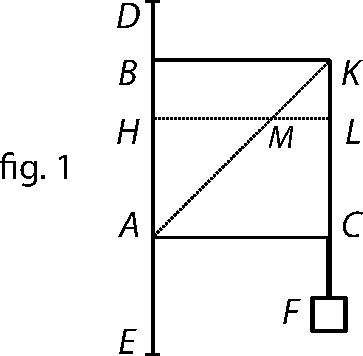
\includegraphics[width=0.47\textwidth]{gesamttex/edit_VIII,3/images/dnr-1a_LH_35_09_16_002-003_d1a.pdf}
\end{minipage}
\hspace{5mm}
\begin{minipage}[t]{0.5\textwidth}
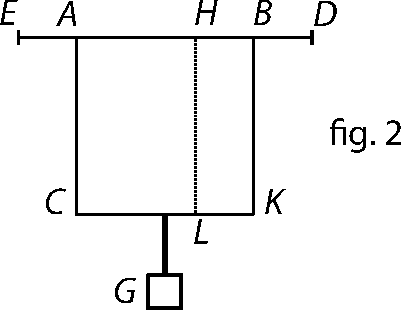
\includegraphics[width=0.52\textwidth]{gesamttex/edit_VIII,3/images/dnr-2a_LH_35_09_16_002-003_d2a.pdf}
\end{minipage}
\\
\\
\hspace*{8mm} [\textit{Fig.~1a, gestr.; L\textsuperscript{1}\! (Bl.~2~r\textsuperscript{o}\!)}]\hspace*{24mm} [\textit{Fig.~2a, gestr.; L\textsuperscript{1}\! (Bl.~2~r\textsuperscript{o}\!)}]\label{LH_35_09_16_002r_Fig_1+2}
\pend
\vspace{1.5em}
\pstart 
\hspace{6mm}\begin{minipage}[t]{0.5\textwidth}
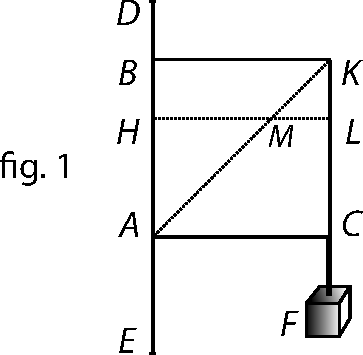
\includegraphics[width=0.54\textwidth]{gesamttex/edit_VIII,3/images/dnr-1b_AE_1684_319-325_d1b.pdf}
\end{minipage}
\hspace{-2mm}
\begin{minipage}[t]{0.5\textwidth}
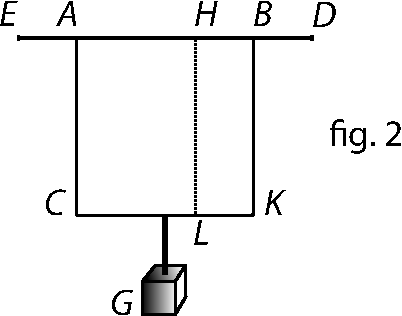
\includegraphics[width=0.58\textwidth]{gesamttex/edit_VIII,3/images/dnr-2b_AE_1684_319-325_d2b.pdf}
\end{minipage}
\\
\\
\hspace*{20mm} [\textit{Fig.~1b; E\textsuperscript{1}}]\hspace*{51mm} [\textit{Fig.~2b; E\textsuperscript{1}}] \label{AE_1684_319-325_Fig.2+3}
\pend
\vspace{2.0em}%	% Diagramm Fig.~1a
%  \centerline{\hspace*{-75mm}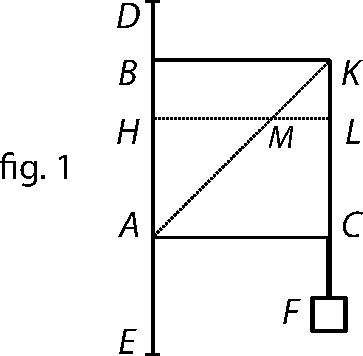
\includegraphics[width=0.22\textwidth]{gesamttex/edit_VIII,3/images/dnr-1a_LH_35_09_16_002-003_d1a.pdf}}%
%  \vspace*{0.5em}
%  \centerline{\hspace*{-65mm}\lbrack\textit{Fig.~1a, gestr.; L\textsuperscript{1}\! (Bl.~2~r\textsuperscript{o}\!)}\rbrack}
%%  \label{}%
%%  \vspace{2.5em}%
%%
%%  \newpage% 
%  \vspace{-9.25em}%	% Diagramm Fig.~2a
%  \centerline{\hspace*{75mm}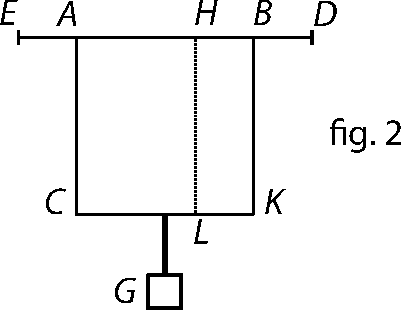
\includegraphics[width=0.24\textwidth]{gesamttex/edit_VIII,3/images/dnr-2a_LH_35_09_16_002-003_d2a.pdf}}%
%  \vspace*{0.5em}
%  \centerline{\hspace*{75mm}\lbrack\textit{Fig.~2a, gestr.; L\textsuperscript{1}\! (Bl.~2~r\textsuperscript{o}\!)}\rbrack}%
%  \label{LH_35_09_16_002r_Fig_1+2}%
%%  \vspace{2.5em}%
%%  \newpage%
%%
%%
%%  \newpage% 
%  \vspace{2.0em}%	% Diagramm Fig.~1b
%  \centerline{\hspace*{-75mm}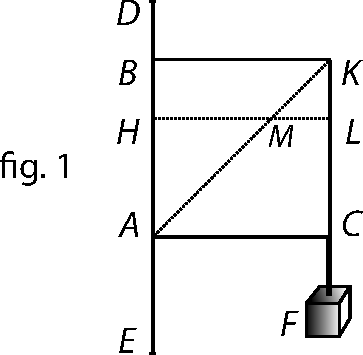
\includegraphics[width=0.28\textwidth]{gesamttex/edit_VIII,3/images/dnr-1b_AE_1684_319-325_d1b.pdf}}%
%  \vspace*{0.5em}
%  \centerline{\hspace*{-65mm}\lbrack\textit{Fig.~1b; E\textsuperscript{1}}\rbrack}%
%%  \label{}%
%%  \vspace{2.0em}%
%%  \newpage%
%%
%%  \newpage% 
%  \vspace{-11.0em}%	% Diagramm Fig.~2b
%  \centerline{\hspace*{75mm}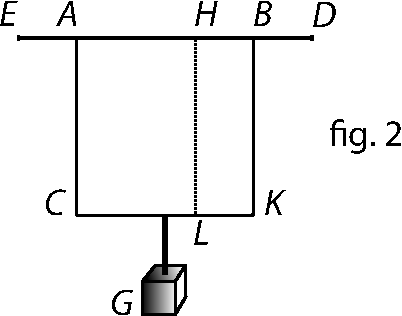
\includegraphics[width=0.30\textwidth]{gesamttex/edit_VIII,3/images/dnr-2b_AE_1684_319-325_d2b.pdf}}%
%  \vspace*{0.5em}
%  \centerline{\hspace*{75mm}\lbrack\textit{Fig.~2b; E\textsuperscript{1}}\rbrack}%
%  \label{AE_1684_319-325_Fig.2+3}%
%  \vspace{2.5em}%
%%  \newpage%
%
%
%%%%    ACHTUNG GETRIXT: folgende Cfootnote bezieht sich eigentlich auf die Abbildungen Fig.~1 und Fig.~2
\pstart% REIN VORLÄUFIG !!!
\edtext{}{\lemma{\hspace{1,6mm}\lbrack\textit{Fig.~1a}\rbrack\ bis \lbrack\textit{Fig.~2b}\rbrack\,}\killnumber\Cfootnote{%
Kein entsprechendes Diagramm ist in \textit{L\textsuperscript{2}} überliefert.}}%
%\pend%
%
% \newpage%
% \vspace*{1.5em}%
%
% \pstart%
% <<<<<<
%
% <
\setline{1}\edtext{}{{\xxref{KZeitz185}{KZeitz186}}%
{%
\lemma{Has \lbrack...\rbrack\ fuit}\Cfootnote{%
Siehe F.\,\textsc{Blondel}, \textit{Epistola ad P.\,W.}, Paris 1661\cite{00337}
(abgedruckt in \textsc{Ders.}, \textit{Résolution des quatre principaux problèmes d'architecture}, Paris 1673, S.~61\textendash69\cite{01230}).}}}%
\edlabel{KZeitz185}Has autem aliasque%
\edlabel{LH_37_03_071v+AE_1684_320_Uebrgng-2}
% \edtext{}{%
% \lemma{Has}\Bfootnote{%autem
% \hspace{-0,5mm}aliasque%
% ~\textit{L\textsuperscript{1}}
% \hspace{0,5mm}Has
% \textit{(1)}~aliamque
% \textit{(2)}~\textbar~autem \textit{erg.}~\textbar\ aliasque%
% ~\textit{L\textsuperscript{2}}}}
% >
id genus
% <
\edtext{Galilaei\protect\index{Namensregister}{\textso{Galilei} (Galilaeus, Galileus), Galileo 1564\textendash1642}
sententias\protect\index{Sachverzeichnis}{sententia}}{%
\lemma{Galilaei}\Bfootnote{%
\hspace{-0,5mm}conclusiones%
~\textit{L\textsuperscript{1}}
\hspace{0,5mm}Galilaei sententias%
~\textit{L\textsuperscript{2}}}}
% >
% <<<
\edtext{Paulus Wurzius,\protect\index{Namensregister}{\textso{W{\"u}rz} (Wurtz, Wurzius), Paul, Baron v. 1612\textendash1676}
%
summis militiae honoribus\protect\index{Sachverzeichnis}{honor militiae}\protect\index{Sachverzeichnis}{militia}
rebusque gestis\protect\index{Sachverzeichnis}{res gestae} non ita pridem clarus,
idemque}{%
\lemma{Paulus}\Bfootnote{%
\textit{(1)}~Wurzius
\textit{(2)}~Würzius
\textit{(a)}~non
\textit{(aa)}~idem
\textit{(bb)}~sum
\textit{(cc)}~ita pridem
\textit{(b)}~summis militiae muneribus rebusque gestis
\textbar~non ita pridem \textit{erg.}~%
\textbar\ clarus, idemque%
~\textit{L\textsuperscript{1}}
%
\hspace{0,5mm}Paulus Würzius
\lbrack...\rbrack\ clarus, idemque
~\textit{L\textsuperscript{2}}
%
\hspace{0,5mm}Paulus Wurzius,
\lbrack...\rbrack\ clarus, idemque%
~\textit{E\textsuperscript{1}}}}
% >>>
horum studiorum\protect\index{Sachverzeichnis}{studium} valde
% <
\edtext{intelligens,}{%
\lemma{intelligens\, \textit{L\textsuperscript{1}\! u.\! L\textsuperscript{2}}}\Bfootnote{%
\hspace{0,5mm}intelligens~,~\textit{E\textsuperscript{1}}}}
% >
experimentis\protect\index{Sachverzeichnis}{experimentum} compluribus sumtis examinare
% <
\edtext{olim}{%
\lemma{olim}\Bfootnote{%
\textit{erg.~L\textsuperscript{1}}}}
% >
aggressus est,
% <
\edtext{successu\protect\index{Sachverzeichnis}{successus}
quibusdam}{%
\lemma{successu}\Bfootnote{%
\hspace{-0,5mm}\textbar~tamen \textit{gestr.}~%
\textbar\ quibusdam%
~\textit{L\textsuperscript{1}}}}
% >
conclusionibus\protect\index{Sachverzeichnis}{conclusio}
parum
\edtext{respondente:}{%
\lemma{respondente~,~\textit{L\textsuperscript{1}}}\Bfootnote{%
respondente\,~\textit{L\textsuperscript{2}}
\hspace{1,0mm}respondente~:~\textit{E\textsuperscript{1}}}}
%
quemadmodum
% <<<
\edtext{}{{\xxref{KZeitz183}{KZeitz184}}%
{%
\lemma{habeo}\Bfootnote{%
\textit{(1)}~ab Exim
\textit{(2)}~a
\textit{(a)}~B
\textit{(b)}~Cl. Blondello in his
\textit{(aa)}~rebus
\textit{(bb)}~aliisque studiis eximio Delphini nuper%
~\textit{L\textsuperscript{1}}
%
\hspace{0,5mm}
habeo a Cl. \lbrack...\rbrack\ studiis eximio, % Blondello 
\textit{(1)}~Delphini nuper
\textit{(2)}~Serenissimi Delphini nuper%
~\textit{L\textsuperscript{2}}
%
\hspace{0,5mm}habeo a
\textbar~CL. \textit{ändert Hrsg. nach L\textsuperscript{1}\! u.\! L\textsuperscript{2}}~%
\textbar\ Blondello \lbrack...\rbrack\ Delphini nuper%
~\textit{E\textsuperscript{1}}}}}%
\edlabel{KZeitz183}habeo a \lbrack Cl.\rbrack\ Blondello\protect\index{Namensregister}{\textso{Blondel}, François 1618\textendash1686}
in his  aliisque
\pend
\newpage
\pstart
\noindent studiis\protect\index{Sachverzeichnis}{studium} eximio,
Serenissimi
\edtext{Delphini%
\protect\index{Namensregister}{\textso{Ludwig} (Grand Dauphin, Delphinus), Thronfolger v. Frankreich 1661\textendash1711}}{%
\lemma{Delphini}\Cfootnote{%
Louis de France (1661\textendash1711), Ludwigs XIV. ältester Sohn und Frankreichs damaliger Thron\-folger.}} %
nuper\edlabel{KZeitz184}
% >>>
in Mathematicis\protect\index{Sachverzeichnis}{mathematica}
% <
\edtext{Magistro,\protect\index{Sachverzeichnis}{magister}}{%
\lemma{Magistro~,~\textit{L\textsuperscript{1}}}\Bfootnote{% \hspace{0,5mm}
Magistro~\textit{L\textsuperscript{2}}
\hspace{1,0mm}Magistro~,~\textit{E\textsuperscript{1}}}}
% >
et Academiae\protect\index{Sachverzeichnis}{Académie Royale d'Architecture}
% ||||
\edlabel{LH_37_03_071v+AE_1684_320_Wurzius-1}Architectonicae directore,
qui idem argumentum\protect\index{Sachverzeichnis}{argumentum} excoluit,
et Wurzio\protect\index{Namensregister}{\textso{W{\"u}rz} (Wurtz, Wurzius), Paul, Baron v. 1612\textendash1676}
familiaris fuit;\edlabel{KZeitz186}
% >>>>>>
sed\edlabel{LH_37_03_071v+AE_1684_320_Wurzius-2}
\edtext{}{%
{\xxref{LH_37_03_071v+AE_1684_320_Wurzius-1}{LH_37_03_071v+AE_1684_320_Wurzius-2}}%
{\lemma{Architectonicae}\Bfootnote{\hspace{-0,5mm}%
\textbar~Parisinae \textit{gestr.}~\textbar\ directore
\textbar~qui
\textit{(1)}~in eodem argumento
\textit{(2)}~idem argumentum excoluit et Wurzio familiaris
\textbar~olim \textit{gestr.}~%
\textbar\ fuit \textit{erg.}~%
\textbar~. Sed%
~\textit{L\textsuperscript{1}}
%
\hspace{0,5mm}Architectonicae Directore,
\lbrack...\rbrack\ fuit. Sed%
~\textit{L\textsuperscript{2}}
%
\hspace{0,5mm}Architectonicae directore,
\lbrack...\rbrack\ fuit; sed~%
\textit{E\textsuperscript{1}}}}}%
% ||||
et Cl.
% <<<<<<
\edtext{Mariottus\protect\index{Namensregister}{\textso{Mariotte}, Edme, Seigneur de Chazeuil ca. 1620\textendash1684}
ex Academia
% <<
\edtext{Regia,\protect\index{Sachverzeichnis}{Academia regia (Académie Royale des Sciences)}
de rebus opticis\protect\index{Sachverzeichnis}{res optica}
et mechanicis\protect\index{Sachverzeichnis}{res mechanica}
praeclare meritus,}{%
\lemma{Regia}\Bfootnote{%
\textbar~de rebus \lbrack...\rbrack\ praeclare meritus \textit{erg.}~\textbar%
~\textit{L\textsuperscript{1}}
%
\hspace{0,5mm}Regia\, de rebus Opticis et Mechanicis praeclare meritus%
~\textit{L\textsuperscript{2}}
%
\hspace{0,5mm}Regia~, de \lbrack... \rbrack\ praeclare meritus,%
~\textit{E\textsuperscript{1}}}}
% >>
experimentis\protect\index{Sachverzeichnis}{experimentum} factis
% <<<
\edtext{comperit,
pondus\protect\index{Sachverzeichnis}{pondus appensum} \textit{F} multo minus,
quam voluit Galilaeus,%
\protect\index{Namensregister}{\textso{Galilei} (Galilaeus, Galileus), Galileo 1564\textendash1642}
ad abrumpendam trabem\protect\index{Sachverzeichnis}{trabs abrumpenda} sufficere.}{%
\lemma{comperit}\Bfootnote{%
pondus \textit{F} in fig.~1 multo minus
\textit{(1)}~esse
\textit{(2)}~quam voluit Galilaeus ad abrumpendam trabem sufficere.%
~\textit{L\textsuperscript{1}}
%
\hspace{0,5mm}comperit\, pondus \textit{F} in fig.~1 multo minus quam voluit Galilaeus ad abrumpendam trabem sufficere.%
~\textit{L\textsuperscript{2}}
%
\hspace{0,5mm}comperit~, pondus \lbrack...\rbrack\ trabem sufficere.%
~\textit{E\textsuperscript{1}}}}
% >>>
Cujus causa\protect\index{Sachverzeichnis}{causa} nulla alia esse
%
\lbrack S.~321\rbrack\ % S.321
%
potest,
quam
% <
\edtext{quod \edlabel{LH_35_09_15_021v_duaehypotheseis-1}is}{%
\lemma{quod}\Bfootnote{%
\hspace{-0,5mm}Galilaeus%
~\textit{L\textsuperscript{1}}
\hspace{0,5mm}quod is%
~\textit{L\textsuperscript{2}}}}
% >
trabem consideravit ut perfecte rigidam,\protect\index{Sachverzeichnis}{trabs perfecte rigida}
quae uno momento\protect\index{Sachverzeichnis}{momentum temporis} tota abrumpatur,
ubi resistentia ejus\protect\index{Sachverzeichnis}{resistentia trabis}
% <
\edtext{superata est,
cum}{%
\lemma{superata est~.}\Bfootnote{%
\hspace{-0,5mm}Cum%
~\textit{L\textsuperscript{1}}
\hspace{0,5mm}superata est~, cum%
~\textit{L\textsuperscript{2}}}}
% >
tamen omnia
% <
\edtext{corpora,\protect\index{Sachverzeichnis}{corpus solidum}}{%
\lemma{corpora\, \textit{L\textsuperscript{1}\! u.\! L\textsuperscript{2}}}\Bfootnote{%
\hspace{0,5mm}corpora~,~\textit{E\textsuperscript{1}}}}
% >
quae nobis tractare
% <<<
\edtext{datum est,
nonnihil cedant,
antequam divelli possint.%
\edlabel{LH_35_09_15_021v_duaehypotheseis-2}}{%
\lemma{datum}\Bfootnote{%
\hspace{-0,5mm}est antequam frangantur aut rumpantur, prius flectantur aut extendantur. \lbrack2~v\textsuperscript{o}\rbrack%%%% Blatt 2v
~\textit{L\textsuperscript{1}}
\hspace{0,5mm}datum est nonnihil cedant antequam divelli possint.%
~\textit{L\textsuperscript{2}}
\hspace{0,5mm}datum est, \lbrack...\rbrack\ divelli possint.%
~\textit{E\textsuperscript{1}}}}
% >>>
Unde Cl. Mariottus\protect\index{Namensregister}{\textso{Mariotte}, Edme, Seigneur de Chazeuil ca. 1620\textendash1684}
\edtext{hoc observans}{%
\lemma{hoc}\Bfootnote{%
\hspace{-0,5mm}observans
\textit{fehlt~L\textsuperscript{1}\! u.\! L\textsuperscript{2}}}}
%
ingenioso
% <
\edtext{calculo\protect\index{Sachverzeichnis}{calculus ingeniosus} collegit,}{%
\lemma{calculo}\Bfootnote{%
\hspace{-0,5mm}conjecit;%
~\textit{L\textsuperscript{1}}
\hspace{0,5mm}calculo collegit,%
~\textit{L\textsuperscript{2}}}}
% >
% <<
\edtext{pondus\protect\index{Sachverzeichnis}{pondus appensum} \textit{F} esse}{%
\lemma{pondus}\Bfootnote{%
\hspace{-0,5mm}\textit{F} in \textso{fig.}~\textso{1} debere esse%
~\textit{L\textsuperscript{1}}
\hspace{0,5mm}pondus \textit{F}
\textbar~in \textso{fig.}~\textso{1} debere \textit{gestr.}~%
\textbar\ esse%
~\textit{L\textsuperscript{2}}% \hspace{0,5mm}
% esse%
% ~\textit{E\textsuperscript{1}}
}}
% >>
circiter quartam partem%
% ||||
\edtext{}{%
{\xxref{LH_37_03_071v+AE_1684_321_pndssed-1}{LH_37_03_071v+AE_1684_321_pndssed-2}}%
{\lemma{ponderis}\Bfootnote{%
\hspace{-0,5mm}\textit{G} in \textso{fig.}~\textso{2.} Quae cum mihi occasionem dedissent%
~\textit{L\textsuperscript{1}}
%
\hspace{0,5mm}ponderis \textit{G}
\textbar~in \textso{fig.}~\textso{2} \textit{gestr.}~%
\textbar~. Sed cum inde mihi data esset occasio%
~\textit{L\textsuperscript{2}}
%
\hspace{0,5mm}ponderis \textit{G}
\lbrack...\rbrack\ esset occasio%
~\textit{E\textsuperscript{1}}}}}
%
\edlabel{LH_37_03_071v+AE_1684_321_pndssed-1}%
ponderis \textit{G}.\protect\index{Sachverzeichnis}{pondus appensum}%
}{%
\lemma{Mariottus \lbrack...\rbrack\ ponderis \textit{G}}\Cfootnote{%
Mariotte hatte seine Kritik an Galileis Berechnung des Verhältnisses zwischen Bruch- und Zugfestigkeit mehrmals an Leibniz mitgeteilt,
etwa in seinen Briefen vom 28. April 1678 und 20. Juli 1682 sowie in seiner % Siehe \textsc{Mariotte}, 
\textit{Dissertation sur la résistance des solides}, Beilage zum Brief vom 25. Ja\-nu\-ar 1683;
vgl. \textit{LSB} \cite{01232}III,~2 N.~163, S.~455f.; \cite{01233}III,~3 N.~376, S.~670f.; \cite{01233}III,~3 N.~437, S.~772\textendash776\cite{01231}
(letzterer Text entspricht mit Anpassungen \textit{MO} II, S.~461\textendash465\cite{01218}).
Siehe oben, S.~\refpassage{AE_1684_319-325_intro_MariotteKritik-1}{AE_1684_319-325_intro_MariotteKritik-2}.}}
% >>>>>>
Sed %
%%%%%%%%%%%%%%%%%%%%%%%%%%%%%%%%%%%%%%%%%%%%%%%%%%%%%%%%%%%%%%%%%%%%%%%%%%%%%%%%
% HS: Großschreibung, weil Satzanfang; Punkt vorhanden, daher triviale Änderung stillschweigend.
% <<<<<
%\edtext{cum inde data mihi esset occasio%
%\protect\index{Sachverzeichnis}{occasio}%
%\edlabel{LH_37_03_071v+AE_1684_321_pndssed-2}
%% ||||
%rem considerandi profundius,
%et
%% <
%\edtext{ad}{%
%\lemma{ad}\Bfootnote{%
%\textit{erg.~L\textsuperscript{1}}}}
%% >
%leges Geometrarum\protect\index{Sachverzeichnis}{lex geometrarum} exigendi,
%veras tandem\protect\index{Sachverzeichnis}{proportio vera} proportiones
%%>
%\edtext{erui,}{%
%\lemma{erui~,~\textit{L\textsuperscript{1}}}\Bfootnote{%
%\hspace{0,5mm}erui\,~\textit{L\textsuperscript{2}}
%\hspace{0,5mm}erui~,~\textit{E\textsuperscript{1}}}}%
%% >
%}{%
%\lemma{cum \lbrack...\rbrack\ erui}\Cfootnote{%
%Anspielung auf die umfangreiche Untersuchung über die Festigkeit der Balken, die Leibniz ab Ende Juli/Anfang August 1682 in Anlehnung an den Briefwechsel mit Mariotte durchgeführt hat.
%Hieraus sind ab Ende Januar 1683 die Texte N.~??Y\textsubscript{1} bis ??Y\textsubscript{9} entstanden.
%Siehe für weitere Details oben, S.~\refpassage{AE_1684_319-325_intro_LeibizAnMariotte-1}{AE_1684_319-325_intro_LeibizAnMariotte-1}\,ff.}} %{AE_1684_319-325_intro_LeibizAnMariotte-2}
%% >>>>>%%%%%%%%%%%%%%%%%%%%%%%%%%%%%%%%%%%%%%%%%%%%%%%%%%%%%%%%%%%%%%%%%%%%%%%%%%%%%%%%%%%%%%%%%%%%%%%%%%%%%%%%%%%%%%%%%%%%%%%%%%%%%%%%%%%%%%%%%%%%%%%%%%%%%%%%%%%%
\edlabel{KZeitz1}%
\edtext{}%
{{\xxref{KZeitz1}{KZeitz2}}%
{%
\lemma{cum \lbrack...\rbrack\ erui}\Cfootnote{%
Anspielung auf die umfangreiche Untersuchung über die Festigkeit der Balken, die Leibniz ab Ende Juli/Anfang August 1682 in Anlehnung an den Briefwechsel mit Mariotte durchgeführt hat.
Hieraus sind ab Ende Januar 1683 die Texte N.~14\textsubscript{1} bis 14\textsubscript{9} entstanden.
Siehe für weitere Details oben, S.~\refpassage{AE_1684_319-325_intro_LeibizAnMariotte-1}{AE_1684_319-325_intro_LeibizAnMariotte-1}\,ff.}}}%
cum inde data mihi esset occasio%
\protect\index{Sachverzeichnis}{occasio}%
\edlabel{LH_37_03_071v+AE_1684_321_pndssed-2}
% ||||
rem considerandi profundius,
et
% <
\edtext{ad}{%
\lemma{ad}\Bfootnote{%
\textit{erg.~L\textsuperscript{1}}}}
% >
leges Geometrarum\protect\index{Sachverzeichnis}{lex geometrarum} exigendi,
veras \makebox[1.0\textwidth][s]{tandem\protect\index{Sachverzeichnis}{proportio vera} proportiones
%>
\edtext{erui,}{%
\lemma{erui~,~\textit{L\textsuperscript{1}}}\Bfootnote{%
\hspace{0,5mm}erui\,~\textit{L\textsuperscript{2}}
\hspace{0,5mm}erui~,~\textit{E\textsuperscript{1}}}}%
% >
\edlabel{KZeitz2} %
%%%%%%%%%%%%%%%%%%%%%%%%%%%%%%%%%%%%%%%%%%%%%%%%%%%%%%%%%%%%%%%%%%%%%%%%%%%%%%%%%%%%%%%%%%%%%%%%%%%%%%%%%%%%%%%%%%%%%%%%%%%%%%%%%%%%%%%%%%%%%%%%%%%%%%%%%%%%%%%%%%
demonstravique inter alia
% <
\edtext{pondus\protect\index{Sachverzeichnis}{pondus appensum} \textit{F} fore}{%
\lemma{pondus}\Bfootnote{%
\hspace{-0,5mm} \textit{F} \textbar~exacte \textit{gestr.}~\textbar\ fore%
~\textit{L\textsuperscript{1}}}}
% >
tertiam partem}
%%%%%%%%%%%%%%%%%%dieser künstliche Seitenumbruch ist notwendig, das sonst das gesamte Stück 13 instabil wird%%%%%%%%%%%%%%%%%%%%
\pend
\newpage
\count\Bfootins=900
\count\Afootins=1000
\count\Cfootins=1000%
\pstart
\noindent
\edlabel{LH_37_03_071v+AE_1684_321_GaliQuod-1}%
% <<<<<<
%
\edtext{}%
{{\xxref{LH_37_03_071v+AE_1684_321_GaliQuod-1}{LH_37_03_071v+AE_1684_321_GaliQuod-2}}%
{\lemma{ponderis \textit{G}~,}\Bfootnote{\hspace{-0,5mm}%
\textit{(1)}~et quod palmarium est in hoc argumento,
\textbar~inveni \textit{erg.}~%
\textbar\ loco trabis parabolicae
\textbar~\textit{BACFB} \textit{erg.}~%
\textbar\ in \textso{fig.~3} quam Galilaeus
\textit{(a)}~aequaliter resistere voluit
\textit{(b)}~attulit,
\textit{(aa)}~\textit{BF}
\textit{(bb)}~revera
\textit{(cc)}~trabem
\textit{(dd)}~revera trabem secari debere secundum lineam rectam
\textbar~\textit{BC} \textit{erg.}~%
\textbar\ sive trabem triangularem \textit{BAC} aequaliter ubique ponderi suo resistere
\textbar~et, si prope murum non frangatur nuspiam fractum iri, in quantamcunque demum longitudinem procurrat \textit{erg.}~%
\textbar~, et proinde si a trabe parallelepipeda \textit{AD} dimidium resecetur, eam hoc situ duplo quam antea firmiorem fore.
Nititur autem haec ratiocinatio\protect\index{Sachverzeichnis}{ratiocinatio} mea Hypothesi\protect\index{Sachverzeichnis}{hypothesis} sequenti:
\textit{(2)}~et proinde \lbrack...\rbrack\ minorem esse, quam visum est Galilaeo.%
% \lbrack\textit{Hieran schließt sich % in L\textsuperscript{1} (Bl.~2~v\textsuperscript{o}\!) der Text N.~??Y\textsubscript{7} an.}\rbrack\
~\textit{L\textsuperscript{1}}
%
\hspace{0,5mm}ponderis \textit{G}~, et proinde
\lbrack...\rbrack\ minorem esse quam voluit Galilaeus.
Quod ita ostendemus. % \hspace{-0,5mm}\textbar~Quod ita ostendemus. \textit{fehlt~E\textsuperscript{1}}~\textbar\, 
\lbrack72~r\textsuperscript{o}\rbrack\ Quod%
~\textit{L\textsuperscript{2}}
%
\hspace{0,5mm}ponderis \textit{G} \lbrack...\rbrack\ Galilaeus.
Quod%
~\textit{E\textsuperscript{1}}}}}%
%
\edtext{ponderis\protect\index{Sachverzeichnis}{pondus appensum} \textit{G}
% \lbrack,\rbrack\
et proinde firmitatem corporum\protect\index{Sachverzeichnis}{firmitas corporis}
rupturae resistentium\protect\index{Sachverzeichnis}{corpus rupturae resistens}
in sesquialtera proportione minorem esse,
quam voluit Galilaeus.\edlabel{LH_37_03_071v_Anfang-2}%
\protect\index{Namensregister}{\textso{Galilei} (Galilaeus, Galileus), Galileo 1564\textendash1642}}{%
\lemma{ponderis \textit{G} \lbrack...\rbrack\ Galilaeus}\Cfootnote{%
Die in der Variante \textit{(1)} von \textit{L\textsuperscript{1}} erwähnte \textit{fig.~3} ist das Diagramm \lbrack\textit{Fig.~5a}\rbrack\ auf S.~\pageref{LH_35_09_16_002r_Fig.5a}.}}%
\edtext{}{\lemma{Galilaeus}\Cfootnote{Hieran schließt sich in \textit{L\textsuperscript{1}} (Bl.~2~v\textsuperscript{o}\!) der Entwurf N.~14\textsubscript{7} an.}}
\pend%
% \vspace{0.5em}%
%
% \pstart%
% \noindent%
% \lbrack\textit{Hieran schließt sich in L\textsuperscript{1} (Bl.~2~v\textsuperscript{o}\!) der Text N.~??Y\textsubscript{7} an.}\rbrack\
% ACHTUNG GETRIXT:
% \edtext{}{%
% \lemma{\hspace{1,6mm}\lbrack\textit{Fig.~3a}\rbrack\ bis \lbrack\textit{Fig.~3c}\rbrack}\killnumber\Cfootnote{%
% Kein entsprechendes Diagramm ist in \textit{L\textsuperscript{1}} überliefert.
% \lbrack\textit{Fig.~3c}\rbrack\ ist lediglich in \textit{E\textsuperscript{1}} überliefert.}}
% \pend%
% \vspace{0.5em}%
%
%
%  \newpage%
%  \vspace*{2.0em}%	% Diagramm Fig.~3a
%  \centerline{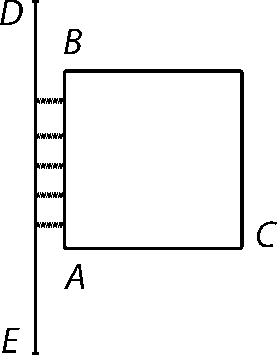
\includegraphics[width=0.16\textwidth]{gesamttex/edit_VIII,3/images/dnr-3a_LH_37_03_071-072_d3a.pdf}}% \hspace*{-100mm}
%  \vspace*{0.5em}
%  \centerline{\lbrack\textit{Fig.~3a, gestr.; L\textsuperscript{2}\! (Bl.~72~r\textsuperscript{o}\!)}\rbrack}% \hspace*{-100mm}
%  \label{}
%  \newpage%
%  \vspace*{2.5em}%
%
%
%  \newpage% 
% \vspace*{0.0em}%	% Diagramm Fig.~3b
%  \centerline{\hspace*{-65mm}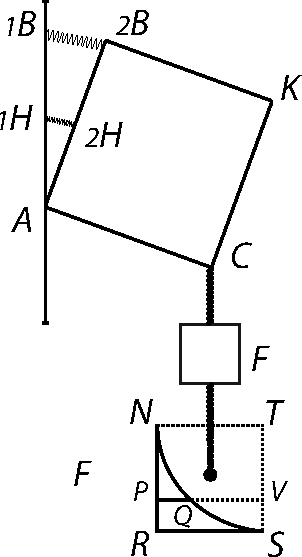
\includegraphics[width=0.24\textwidth]{gesamttex/edit_VIII,3/images/dnr-3b_LH_37_03_071-072_d3b.pdf}}%
%  \vspace*{1.0em}
%  \centerline{\hspace*{-65mm}\lbrack\textit{Fig.~3b; L\textsuperscript{2}\! (Bl.~72~r\textsuperscript{o}\!)}\rbrack}%
% %  \label{}%
%  \vspace{-1.25em}%
%  \newpage%
%
%
%  \newpage% 
% \vspace{-16.0em}%	% Diagramm Fig.~3c
%  \centerline{\hspace*{65mm}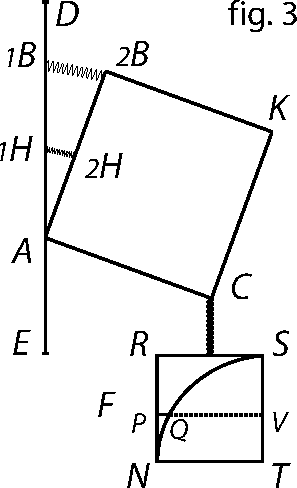
\includegraphics[width=0.30\textwidth]{gesamttex/edit_VIII,3/images/dnr-3c_AE_1684_319-325_d3c.pdf}}%
%  \vspace*{1.0em}
%  \centerline{\hspace*{65mm}\lbrack\textit{Fig.~3c; E\textsuperscript{1}}\rbrack}%
%  \label{AE_1684_321_Fig_3c}%
%  \vspace{2.0em}%
%  \newpage%
% ACHTUNG GETRIXT:
%\pstart%
%\phantom{X}%
%\edtext{}{%
%\lemma{\hspace{1,6mm}\lbrack\textit{Fig.~3a}\rbrack\ bis \lbrack\textit{Fig.~3c}\rbrack}\killnumber\Cfootnote{%
%Kein entsprechendes Diagramm ist in \textit{L\textsuperscript{1}} überliefert.
%\lbrack\textit{Fig.~3c}\rbrack\ ist lediglich in \textit{E\textsuperscript{1}} überliefert.}}
%\pend%
%\newpage
%
\pstart%
\edtext{}{%
{\xxref{LH_37_03_071-072+AE_1684_319-325_L1omissa_rjsuv-1}{LH_37_03_071-072+AE_1684_319-325_L1omissa_rjsuv-2}}%
{\lemma{Quod}\Bfootnote{%
\hspace{-0,5mm}ut \lbrack...\rbrack\ esse Parabolicam.
\textit{fehlt~L\textsuperscript{1}}}}}%
Quod ut %
\edlabel{LH_37_03_071v+AE_1684_321_GaliQuod-2}%
\edlabel{LH_37_03_071v+AE_1684_321_mox_ourihb-1}%
\edlabel{LH_35_09_15_021v_duaehypotheseis-3}%
\edlabel{LH_37_03_071-072+AE_1684_319-325_L1omissa_rjsuv-1}
\edtext{intelligatur,}{%
\lemma{intelligatur~\textit{L\textsuperscript{2}}}\Bfootnote{%
\hspace{0,5mm}intelligatur~,~\textit{E\textsuperscript{1}}}}
% >
ante omnia
% <<
\edtext{sciendum est,
corpora duo cohaerentia\protect\index{Sachverzeichnis}{corpora cohaerentia}
non statim uno momento\protect\index{Sachverzeichnis}{momentum temporis} a se invicem tota divelli;%
\edlabel{LH_35_09_15_021v_duaehypotheseis-4}
quod judicari potest}{%
\lemma{sciendum}\Bfootnote{%
\hspace{-0,5mm}\textbar~est \textit{erg.}~%
\textbar\ corpora duo
\textbar~cohaerentia \textit{erg.}~%
\textbar\ non statim a se invicem uno momento tota divelli,
\textit{(1)}~patet
\textit{(2)}~intelligi potest
\textit{(3)}~quod
\textit{(a)}~intelligi potest
\textit{(b)}~judicari potest%
~\textit{L\textsuperscript{2}}
\hspace{0,5mm}sciendum est, \lbrack...\rbrack\ judicari potest%
~\textit{E\textsuperscript{1}}}}
% >>
exemplo\protect\index{Sachverzeichnis}{exemplum}
% <
\edtext{baculi\protect\index{Sachverzeichnis}{baculus flexus}}{%
\lemma{baculi~,~\textit{L\textsuperscript{2}}}\Bfootnote{%
\hspace{0,5mm}baculi~\textit{E\textsuperscript{1}}}}
% >
qui flectitur antequam frangatur,
et exemplo\protect\index{Sachverzeichnis}{exemplum} chordae\protect\index{Sachverzeichnis}{chorda extensa}
quae
% <
\edtext{extenditur,}{%
\lemma{extenditur~\textit{L\textsuperscript{2}}}\Bfootnote{%
\hspace{0,5mm}extenditur~,~\textit{E\textsuperscript{1}}}}
% >
antequam
% <
\edtext{rumpatur;}{%
\lemma{rumpatur~,~\textit{L\textsuperscript{2}}}\Bfootnote{%
\hspace{0,5mm}rumpatur~;~\textit{E\textsuperscript{1}}}}
% >
et ipsa flexio baculi\protect\index{Sachverzeichnis}{flexio baculi}
est quaedam extensio in convexa ejus superficie.\protect\index{Sachverzeichnis}{extensio superficiei}
% <<<<
\edtext{Nihilque tam rigidum
% <
\edtext{esse,}{%
\lemma{esse~\textit{L\textsuperscript{2}}}\Bfootnote{%
\hspace{0,5mm}esse~,~\textit{E\textsuperscript{1}}}}
% >
quin levi etiam impulsu\protect\index{Sachverzeichnis}{impulsus levis} flectatur nonnihil,
ex natura soni\protect\index{Sachverzeichnis}{natura soni}\protect\index{Sachverzeichnis}{sonus} sequitur,
qui tremor\protect\index{Sachverzeichnis}{tremor} est
% <
\edtext{quidam,}{%
\lemma{quidam~\textit{L\textsuperscript{2}}}\Bfootnote{%
\hspace{0,5mm}quidam~,~\textit{E\textsuperscript{1}}}}
% >
sive flexio\protect\index{Sachverzeichnis}{flexio reciprocata}
% <<
\edtext{reciprocata partium corporis sonantis,\protect\index{Sachverzeichnis}{corpus sonans}}{%
\lemma{reciprocata}\Bfootnote{%
\textit{(1)}~corporis sonantis
\textit{(2)}~partium corporis sonantis%
~\textit{L\textsuperscript{2}}
\hspace{0,5mm}reciprocata partium corporis sonantis,%
~\textit{E\textsuperscript{1}}}}%
% >>
}{\lemma{Nihilque \lbrack...\rbrack\ sonantis}\Cfootnote{%
Siehe die Ausführungen über die Entstehung und Übertragung des Schalls in N.~12\textsubscript{1} bis N.~12\textsubscript{3}.}}
% >>>>
% <<<<
\edtext{%
%
licet\edtext{ eo promtior atque insensibilior sit restitutio\protect\index{Sachverzeichnis}{restitutio insensibilis}
acutiorque sonus,\protect\index{Sachverzeichnis}{sonus acutus}
quo partes tremulae\protect\index{Sachverzeichnis}{pars tremula}
sunt breviores et magis tensae,\protect\index{Sachverzeichnis}{pars tensa}
corpusque\protect\index{Sachverzeichnis}{corpus sonans} durius constituunt.}{%
\lemma{licet}\Bfootnote{%
\hspace{-0,5mm}eo promtior
\textbar~atque insensibilior \textit{erg.}~\textbar\
sit restitutio acutiorque sonus, quo
\textit{(1)}~corpus est
\textit{(2)}~partes tremulae sunt
\textit{(a)}~rigidiores et
\textit{(b)}~breviores et \lbrack...\rbrack\ durius constituunt.
\textit{erg.~L\textsuperscript{2}}}}%
}{\lemma{licet \lbrack...\rbrack\ constituunt}\Cfootnote{%
Siehe hierüber N.~12\textsubscript{3}, S.~\refpassage{LH_37_01_006v_sa1}{LH_37_01_006v_clappans-2}.}}
% >>>>
Vitrum ipsum flexile\protect\index{Sachverzeichnis}{vitrum flexile}
% <
\edtext{esse probant filamenta\protect\index{Sachverzeichnis}{filamentum vitri} ejus longa et tenuia;}{%
\lemma{esse}\Bfootnote{%
\textit{(1)}~ostendunt tenuia
\textit{(2)}~probant ejus filamenta
\textit{(a)}~dur
\textit{(b)}~longa et tenuia;%
~\textit{L\textsuperscript{2}}
\hspace{0,5mm}esse probant \lbrack...\rbrack\ et tenuia;% filamenta ejus longa
~\textit{E\textsuperscript{1}}}}
% >
%
\makebox[1.0\textwidth][s]{\edtext{}{{\xxref{KZeitz187}{KZeitz188}}%
{%
\lemma{quomodo \lbrack...\rbrack\ ostendunt}\Cfootnote{%
Siehe \cite{00143}L.~\textsc{Magalotti}, \textit{Saggi di naturali esperien\-ze}, Florenz 1666, S.~186: \glqq Terza esperienza circa un effetto del caldo e del freddo\grqq.
Zu diesem % bei der Accademia del Cimento durchgeführten 
Versuch über die Dehnung und Zusammenziehung eines Gefäßes aus Kristall finden sich in \textit{LSB} VIII,~1 N.~37\cite{01100} keine Auszüge von Leibniz. Siehe jedoch seine Bemerkung (ebd. S.~283.7\textendash8\cite{01100}) zu einem ähnlichen Versuch der Accademia del Cimento.}}}%
\edlabel{KZeitz187}quomodo
\edtext{vitrum satis crassum\protect\index{Sachverzeichnis}{vitrum frigore contractum}}{%
\lemma{vitrum}\Bfootnote{%
\hspace{-0,5mm}satis crassum
\textit{erg.~L\textsuperscript{2}}}}
%
frigore\protect\index{Sachverzeichnis}{frigus}
% <
\edtext{contrahatur,}{%
\lemma{contrahatur~\textit{L\textsuperscript{2}}}\Bfootnote{%
\hspace{0,5mm}contrahatur~,~\textit{E\textsuperscript{1}}}}
% >
experimenta Florentina\protect\index{Sachverzeichnis}{experimentum Florentinum} ostendunt.\edlabel{KZeitz188}}
\pend
\newpage
\pstart
\noindent 
%
Partes quidem plantarum\protect\index{Sachverzeichnis}{pars plantae}
et animalium\protect\index{Sachverzeichnis}{pars animalis}
quodammodo textiles\protect\index{Sachverzeichnis}{pars textilis}
% <
\edtext{esse,}{%
\lemma{esse~\textit{L\textsuperscript{2}}}\Bfootnote{%
\hspace{0,5mm}esse~,~\textit{E\textsuperscript{1}}}}
% >
et ex filamentis\protect\index{Sachverzeichnis}{filamentum} varie implicatis
% <
\edtext{constare,}{%
\lemma{constare~\textit{L\textsuperscript{2}}}\Bfootnote{%
\hspace{0,5mm}constare~,~\textit{E\textsuperscript{1}}}}
% >
sensu\protect\index{Sachverzeichnis}{sensus}
\edtext{ipso docemur.}{%
\lemma{ipso}\Bfootnote{%
\textit{(1)}~constat.
\textit{(2)}~docemur.%
~\textit{L\textsuperscript{2}}}}
%
Mineralia\protect\index{Sachverzeichnis}{mineralis} quoque et metalla\protect\index{Sachverzeichnis}{metallum}
cum fluida
% <
\edtext{essent,}{%
\lemma{essent~\textit{L\textsuperscript{2}}}\Bfootnote{%
\hspace{0,5mm}essent~,~\textit{E\textsuperscript{1}}}}
% >
postea congelata
\count\Bfootins=1100
\count\Afootins=1100
\count\Cfootins=1100
% <<
\edtext{sunt,
et eadem nunc quoque habere tenacitatem\protect\index{Sachverzeichnis}{tenacitas}
et in fila\protect\index{Sachverzeichnis}{filum} duci,
malleoque\protect\index{Sachverzeichnis}{malleus} extendi,
atque in fusione\protect\index{Sachverzeichnis}{fusio} adhaerescere patet.}{%
\lemma{sunt~;}\Bfootnote{\hspace{-0,5mm}%
\textit{(1)}~fluida autem habere tenacitatem et
\textit{(a)}~in
\textit{(b)}~quodammodo in fila duci, ignit
\textit{(2)}~et eadem \textbar~nunc quoque \textit{erg.}~%
\textbar\ cum igne valido fluunt,
\textit{(3)}~et eadem \lbrack...\rbrack\ fila duci % nunc quoque habere tenacitatem et in
\textit{(a)}~patet, cum valido igne fluunt.
\textit{(b)}~malleoque extendi et in fusione
\textit{(aa)}~tenacitatem
\textit{(bb)}~adhaerescere patet.%
~\textit{L\textsuperscript{2}}
\hspace{0,5mm}sunt~, et \lbrack...\rbrack\ adhaerescere patet.%
~\textit{E\textsuperscript{1}}}}
% >>
Consideremus ergo
\edtext{velut fibras\protect\index{Sachverzeichnis}{fibra} quasdam
quae partes corporum connectant, et}{%
\lemma{velut}\Bfootnote{%
\textit{(1)}~chordas
\textit{(2)}~fibras
\textit{(3)}~fibras quasdam
\textit{(a)}~connectentes,
\textit{(b)}~$\langle$\textendash\ quae$\rangle$ partes corporis % ??compositas
\textit{(c)}~quae partes corporum connectant,
\textbar~eo in loco ubi fieri debet ruptura, \textit{gestr.}~%
\textbar\ et%
~\textit{L\textsuperscript{2}}}}
%
\edtext{intelligamus trabem\protect\index{Sachverzeichnis}{trabs alligata}}{%
{\lemma{intelligamus}\Bfootnote{\hspace{-0,5mm}%
\textbar~ergo \textit{gestr.}~%
\textbar~\textso{in fig.}~\textso{1} % \textit{fehlt~E\textsuperscript{1}}~\textbar\ %
trabem~\textit{L\textsuperscript{2}}
\hspace{0,5mm}intelligamus trabem~\textit{E\textsuperscript{1}}}}%
{\lemma{intelligamus trabem}\Cfootnote{%
Die in \textit{L\textsuperscript{2}} erwähnte \textit{fig.~1} ist offenbar das Diagramm \lbrack\textit{Fig.~3b}\rbrack\ auf S.~\pageref{AE_1684_321_Fig_3b}.}}}
%
\edtext{\textit{BC} parieti\protect\index{Sachverzeichnis}{paries}
vel sustentaculo\protect\index{Sachverzeichnis}{sustentaculum trabis} \textit{DE}}{%
\lemma{\textit{BC}}\Bfootnote{%
\textit{(1)}~muro \textit{DE} a
\textit{(2)}~parieti vel sustentaculo \textit{DE}%
~\textit{L\textsuperscript{2}}}}
%
\edtext{plurimis fibrarum plexibus\protect\index{Sachverzeichnis}{plexus fibrae}}{%
\lemma{plurimis}\Bfootnote{%
\textit{(1)}~nodis\protect\index{Sachverzeichnis}{nodus}
\textit{(2)}~nodis \textbar~seu \textit{erg.}~\textbar\ 
\textit{(3)}~fibrarum plexibus%
~\textit{L\textsuperscript{2}}}}
%
alligari in punctis \textit{A}, \textit{H}, \textit{B}, et aliis intermediis innumeris.
Appenso jam
\edtext{pondere\protect\index{Sachverzeichnis}{pondus appensum} \textit{F},}{%
\lemma{pondere}\Bfootnote{\hspace{-0,5mm}%
\textit{F}~\textit{L\textsuperscript{2}}
\hspace{0,5mm}pondere \textit{F},~\textit{E\textsuperscript{1}}}}
%
movebitur nonnihil trabs circa fulcrum\protect\index{Sachverzeichnis}{fulcrum} \textit{A},
\edtext{in\textso{ }\protect\index{Sachverzeichnis}{figura}%
\edtext{\textso{fig.}~\textso{3,}%
}{\lemma{\textso{fig.}~\textso{3}}\Cfootnote{%
Das Diagramm \lbrack\textit{\textit{Fig.~3c}}\rbrack\ auf S.~\pageref{AE_1684_321_Fig_3c}.}}%
}{%
\lemma{in}\Bfootnote{%
\hspace{-0,5mm}\textso{fig.}~\textso{3,}
\textit{fehlt~L\textsuperscript{2}}}}
%
et punctum
\edtext{trabis \textit{B}
a pariete\protect\index{Sachverzeichnis}{paries} discedens\protect\index{Sachverzeichnis}{trabs discedens}
a puncto parietis \textit{{\scriptsize1}B},
veniet ad punctum a pariete\protect\index{Sachverzeichnis}{paries} distans \textit{{\scriptsize2}B},}{%
\lemma{trabis \textit{B}}\Bfootnote{\hspace{-0,5mm}%
\textit{(1)}~ex loco parietis \textit{{\scriptsize1}B} descendet
\textit{(a)}~in
\textit{(b)}~ad \textit{{\scriptsize2}B},
\textit{(2)}~a pariete \lbrack...\rbrack\ distans \textit{{\scriptsize2}B},%
~\textit{L\textsuperscript{2}}}}
%
\edtext{secumque trahens fibram\protect\index{Sachverzeichnis}{fibra tensa}
qua parieti\protect\index{Sachverzeichnis}{paries} annectitur,
eam tendet instar chordae,\protect\index{Sachverzeichnis}{chorda tensa}
sive ultra naturalem suum statum\protect\index{Sachverzeichnis}{status naturalis} extendet
in lineam \textit{{\scriptsize 1}B{\scriptsize 2}B}:
eodemque}{%
\lemma{secumque}\Bfootnote{\hspace{-0,5mm}%
\textit{(1)}~extendet chordam in \textit{{\scriptsize 1}B{\scriptsize 2}B}
\textit{(2)}~trahens fibram qua
\textit{(a)}~parieti
\textit{(b)}~in \textit{B} pari
\textit{(c)}~parieti annectitur,
\textit{(aa)}~et
\textit{(bb)}~eam tendet, sive ultra \lbrack...\rbrack\ statum extendet % naturalem suum
\textit{(aaa)}~ex \textit{{\scriptsize 1}B}
\textit{(bbb)}~in lineam \textit{{\scriptsize 1}B{\scriptsize 2}B}. Eodemque%
~\textit{L\textsuperscript{2}}
\hspace{0,5mm}secumque trahens \lbrack...\rbrack\ \textit{{\scriptsize 1}B{\scriptsize 2}B}: eodemque%
~\textit{E\textsuperscript{1}}}}
%
modo
\edtext{punctum \textit{H} fibram\protect\index{Sachverzeichnis}{fibra tensa} suam}{%
\lemma{punctum \textit{H}}\Bfootnote{%
\hspace{-0,5mm}\textbar~translatum ex \textit{{\scriptsize 1}H} \textit{gestr.}~\textbar\
\textit{(1)}~chordam
\textit{(2)}~fibram suam%
~\textit{L\textsuperscript{2}}}}
%
tendet in
\edtext{\textit{{\scriptsize 1}H{\scriptsize 2}H},
quae lineae licet revera sint insensibiles,\protect\index{Sachverzeichnis}{linea insensibilis}
tamen docendi causa visibilter exhibentur,}{%
\lemma{\textit{{\scriptsize 1}H{\scriptsize 2}H}~:}\Bfootnote{\hspace{-0,5mm}%
\textbar~quae lineae \lbrack...\rbrack\ causa visibilter
\textit{(1)}~repraesentantur
\textit{(2)}~exhibentur
\textit{erg.}~\textbar%
~\textit{L\textsuperscript{2}}
\hspace{0,5mm}\textit{{\scriptsize 1}H{\scriptsize 2}H}~, quae \lbrack...\rbrack\ visibilter exhibentur,%
~\textit{E\textsuperscript{1}}}}
%
%
\lbrack S.~322\rbrack\ % S.~322
%
et
\edtext{quidem
\edtext{\edlabel{AE_1684_322,1_corrige-1}\lbrack fibra\rbrack\edlabel{AE_1684_322,1_corrige-2}%
\protect\index{Sachverzeichnis}{fibra tensa}}{%
\lemma{\lbrack fibra\rbrack}\Cfootnote{%
Siehe die Liste der Korrigenda in N.~14\textsubscript{10}, S.~\refpassage{AE_1684_322,1_corrige-3}{AE_1684_322,1_corrige-4}.
Diese Verbesserung ist auch in \textit{LSB} III,~4 N.~72, S.~181.26\textendash27\cite{01257} als erwünscht vermerkt.%
% hatte Leibniz zunächst in einem verworfenen Konzept seines wohl in der ersten Oktoberhälfte 1684 verfassten Briefes für die \textit{Acta eruditorum} vermerkt; vgl. 
}}}{%
\lemma{quidem}\Bfootnote{\hspace{-0,5mm}%
\textit{(1)}~chorda
\textit{(2)}~fibra%
~\textit{L\textsuperscript{2}}
\hspace{0,5mm}quidem
\textbar~fibris \textit{ändert Hrsg. nach L\textsuperscript{2} u. N.~14\textsubscript{10},
S.~\refpassage{AE_1684_322,1_corrige-3}{AE_1684_322,1_corrige-4}}~\textbar%
~\textit{E\textsuperscript{1}}}}
%
\textit{{\scriptsize 1}H{\scriptsize 2}H}
\edtext{minus resistet trahenti,
quam fibra\protect\index{Sachverzeichnis}{fibra tensa}}{%
\lemma{minus}\Bfootnote{\hspace{-0,5mm}%
\textit{(1)}~\textbar~trahenti \textit{erg.}~%
\textbar\ resistet quam
\textit{(2)}~resistet trahenti quam
\textit{(a)}~chorda
\textit{(b)}~fibra%
~\textit{L\textsuperscript{2}}
\hspace{0,5mm}minus resistet trahenti, quam fibra%
~\textit{E\textsuperscript{1}}}}
%
\textit{{\scriptsize 1}B{\scriptsize 2}B},
\edtext{idque}{%
\lemma{idque}\Bfootnote{%
\textit{erg.~L\textsuperscript{2}}}}
%
in duplicata ratione distantiae ab \textit{A},
\edtext{seu ex duplici capite a distantia sum\-to.}{%
\lemma{seu}\Bfootnote{%
\hspace{-0,5mm}ex \lbrack...\rbrack\ distantia sum\-to
\textit{erg.~L\textsuperscript{2}}}}
%
Nam\textso{ }%
\edtext{}{{\xxref{KZeitz189}{KZeitz190}}%
{%
\lemma{\textso{primo}}\Bfootnote{\hspace{-0,5mm}%
\textit{(1)}~etsi chordae \textit{{\scriptsize 1}B{\scriptsize 2}B}, et \textit{{\scriptsize 1}H{\scriptsize 2}H} eodem modo essent tendendae pondere appenso in \textit{C}, tamen pondere
\textit{(2)}~pondus
\textit{(a)}~\textit{C} q
\textit{(b)}~in \textit{C} quo opus esset ad tendendam
\textit{(aa)}~chordam
\textit{(bb)}~fibram \textit{{\scriptsize 1}H{\scriptsize 2}H} tantundem quantum
\textit{(aaa)}~chordam
\textit{(bbb)}~fibram \textit{{\scriptsize 1}B{\scriptsize 2}B},%
~\textit{L\textsuperscript{2}}
\hspace{0,5mm}\textso{primo} pondus \lbrack...\rbrack\ fibram \textit{{\scriptsize 1}B{\scriptsize 2}B},%
~\textit{E\textsuperscript{1}}}}}%
\edlabel{KZeitz189}\textso{primo }pondus\protect\index{Sachverzeichnis}{pondus appensum} in \textit{C},
quo opus esset ad tendendam fibram\protect\index{Sachverzeichnis}{fibra tensa} \textit{{\scriptsize 1}H{\scriptsize 2}H} tantundem, quan-
\pend
\newpage
\pstart
\noindent quantum fibram\protect\index{Sachverzeichnis}{fibra tensa} \textit{{\scriptsize 1}B{\scriptsize 2}B},\edlabel{KZeitz190}
%
foret minus pondere\protect\index{Sachverzeichnis}{pondus tendens} requisito ad
\edtext{tendendam fibram\protect\index{Sachverzeichnis}{fibra tensa}}{%
\lemma{tendendam}\Bfootnote{%
\textit{(1)}~chordam
\textit{(2)}~fibram%
~\textit{L\textsuperscript{2}}}}
%
\textit{{\scriptsize 1}B{\scriptsize 2}B},
in ratione \textit{AH}
\edtext{ad \textit{AB}: verbi gratia}{%
\lemma{ad}\Bfootnote{\hspace{-0,5mm}%
\textit{AB}~,
\textit{(1)}~seu
\textit{(2)}~verbi gratia%
~\textit{L\textsuperscript{2}}
\hspace{0,5mm}ad \textit{AB}~: verbi gratia%
~\textit{E\textsuperscript{1}}}}
%
si \textit{AH} sit tertia pars
% <<<
\edtext{ipsius \textit{AB},
tunc et pondus\protect\index{Sachverzeichnis}{pondus appensum} in \textit{C},
quod solam fibram\protect\index{Sachverzeichnis}{fibra tensa} \textit{{\scriptsize 1}H{\scriptsize 2}H}
ita extendere potest,
ut fiat aequalis ipsi \textit{{\scriptsize 1}B{\scriptsize 2}B},
erit tertia pars ponderis tendentis\protect\index{Sachverzeichnis}{pondus tendens}
solam fibram\protect\index{Sachverzeichnis}{fibra tensa} \textit{{\scriptsize 1}B{\scriptsize 2}B}.}{%
\lemma{ipsius}\Bfootnote{%
\hspace{-0,5mm}\textit{AB},
\textit{(1)}~opus erit tantum tertia ponderis parte,
\textit{(a)}~ad
\textit{(b)}~in \textit{C}, ad efficiendum, ut chorda \textit{{\scriptsize 1}H{\scriptsize 2}H}
\textbar~sola \textit{erg.}~%
\textbar\ extendatur, quantum chorda
\textit{(2)}~etiam
\textit{(3)}~tunc et pondus in \textit{C} quod solam
\textit{(a)}~chordam
\textit{(b)}~fibram \textit{{\scriptsize 1}H{\scriptsize 2}H}
\textit{(aa)}~extendere potest tantundem qua
\textit{(bb)}~ita extendere potest
\textit{(aaa)}~ut \textit{{\scriptsize 1}H{\scriptsize 2}H} sit
\textit{(bbb)}~ut
\textit{(ccc)}~ut fiat aequalis ipsi
\textbar~chordae \textit{erg. u. gestr.}~%
\textbar\ \textit{{\scriptsize 1}B{\scriptsize 2}B}, erit \lbrack...\rbrack\ tendentis solam
\textit{(aaaa)}~chordam
\textit{(bbbb)}~fibram \textit{{\scriptsize 1}B{\scriptsize 2}B}.%
~\textit{L\textsuperscript{2}}
\hspace{0,5mm}ipsius \textit{AB}, \lbrack...\rbrack\ fibram \textit{{\scriptsize 1}B{\scriptsize 2}B}.%
~\textit{E\textsuperscript{1}}}}
% >>>
Verum
% <<
\edtext{nunc\textso{ secundo }cum ambae simul tenduntur
a pondere appenso\protect\index{Sachverzeichnis}{pondus appensum} in \textit{C},
utique fibra\protect\index{Sachverzeichnis}{fibra tensa} \textit{{\scriptsize 1}H{\scriptsize 2}H}}{%
\lemma{nunc}\Bfootnote{\hspace{-0,5mm}%
\textbar~\textso{secundo} cum ambae simul tenduntur \textit{erg.}~\textbar\
% ~a pondere \lbrack...\rbrack\ \textit{C}, utique \textit{fehlt}~\textbar\
\textit{(1)}~chorda
\textit{(2)}~fibra \textit{{\scriptsize 1}H{\scriptsize 2}H}%
~\textit{L\textsuperscript{2}}\hspace{0,5mm}
nunc \textso{secundo} \lbrack...\rbrack\ fibra \textit{{\scriptsize 1}H{\scriptsize 2}H}%
~\textit{E\textsuperscript{1}}}}
% >>
non est tantum tensa
% <
\edtext{quantum fibra\protect\index{Sachverzeichnis}{fibra tensa}}{%
\lemma{quantum}\Bfootnote{\hspace{-0,5mm}%
\textit{(1)}~chorda
\textit{(2)}~fibra%
~\textit{L\textsuperscript{2}}}}
% >
% <<
\edtext{\textit{{\scriptsize 1}B{\scriptsize 2}B},
sed multo minus, idque rursus in ratione}{%
\lemma{\textit{{\scriptsize 1}B{\scriptsize 2}B},}\Bfootnote{%
\textit{(1)}~sed est tantum ten
\textit{(2)}~sed minus tensa,
\textit{(a)}~in ratione
\textit{(b)}~idque rursus in ratione%
~\textit{L\textsuperscript{2}}
\hspace{0,5mm}\textit{{\scriptsize 1}B{\scriptsize 2}B}, sed \lbrack...\rbrack\ in ratione%
~\textit{E\textsuperscript{1}}}}
% >>
\textit{AH} ad \textit{AB},
nam si \textit{AH} sit tertia pars ipsius \textit{AB},
erit \textit{{\scriptsize 1}H{\scriptsize 2}H} tertia pars ipsius \textit{{\scriptsize 1}B{\scriptsize 2}B}.
Itaque
%%%% HIERZU ANMERKUNG IN DEN INDICES
\edlabel{AE_1684_319-325_a1}%
\edtext{(\protect\vphantom)%
\edtext{ex hypothesi\protect\index{Sachverzeichnis}{hypothesis}
alibi confirmata,
quod extensiones\protect\index{Sachverzeichnis}{extensio}
sint viribus tendentibus\protect\index{Sachverzeichnis}{vis tendens} proportionales}{%
\lemma{ex hypothesi \lbrack...\rbrack\ proportionales}\Cfootnote{Anspielung auf den Text N.~14\textsubscript{7}, der ursprünglich das Teilkonzept N.~14\textsubscript{6},~\textit{L\textsuperscript{1}} fortsetzte und von Leibniz in \textit{Demonstratio quod extensiones Elasticorum sint viribus tendentibus proportionales} umbenannt wurde.}}%
\protect\vphantom()}{%
\lemma{(\protect\vphantom)ex}\Bfootnote{%
\hspace{-0,5mm}hypothesi alibi
\textbar~demonstrata et experimentis\protect\index{Sachverzeichnis}{experimentum} \textit{gestr.}~%
\textbar\ confirmata, quod \lbrack...\rbrack\ tendentibus proportionales\protect\vphantom()
\textit{erg.~L\textsuperscript{2}}}}%
\edlabel{AE_1684_319-325_a2}
%%%% HIERZU ANMERKUNG IN DEN INDICES
ad eam\protect\index{Sachverzeichnis}{fibra tensa} ita tendendam tertia
% <<
\edtext{tantum ponderis\protect\index{Sachverzeichnis}{pondus tendens} parte}{%
\lemma{tantum}\Bfootnote{\hspace{-0,5mm}%
parte \textbar~ponderis \textit{erg.}~\textbar%
~\textit{L\textsuperscript{2}}
\hspace{0,5mm}tantum ponderis parte%
~\textit{E\textsuperscript{1}}}}
% >>
opus erit,
% <<<
\edtext{qua ad eam,
tantundem quantum \textit{{\scriptsize 1}B{\scriptsize 2}B},
tendendam opus fuisset;
id est}{%
\lemma{qua}\Bfootnote{\hspace{-0,5mm}%
\textit{(1)}~opus erat ad tendendam ad
\textit{(2)}~ad \textit{{\scriptsize 1}H{\scriptsize 2}H} tantundem tendendam
\textbar~quantum \textit{{\scriptsize 1}B{\scriptsize 2}B} \textit{erg.}~%
\textbar\ opus fuisset,
\textit{(a)}~haec autem erat
\textit{(b)}~id est%
~\textit{L\textsuperscript{2}}
\hspace{0,5mm}qua ad \lbrack...\rbrack\ id est%
~\textit{E\textsuperscript{1}}}}
% >>>
tertia parte tertiae
% <<
\edtext{partis ponderis\protect\index{Sachverzeichnis}{pondus tendens}
ipsam\protect\index{Sachverzeichnis}{fibra tensa}
\textit{{\scriptsize 1}B{\scriptsize 2}B} tendentis}{%
\lemma{partis}\Bfootnote{\hspace{-0,5mm}%
ipsius ponderis
\textbar~ipsam \textit{erg.}~%
\textbar\ \textit{{\scriptsize 1}B{\scriptsize 2}B} tendentis,%
~\textit{L\textsuperscript{2}}
\hspace{0,5mm}partis ponderis ipsam \textit{{\scriptsize 1}B{\scriptsize 2}B} tendentis%
~\textit{E\textsuperscript{1}}}}
% >>
seu parte ejus
% <<<
\edtext{nona.
Itaque \edlabel{LH_35_09_15_021v_Verweis_Quadrat-1}generaliter in hac simultanea tensione\protect\index{Sachverzeichnis}{tensio simultanea}
omnium fibrarum\protect\index{Sachverzeichnis}{tensio fibrae}\protect\index{Sachverzeichnis}{fibra tensa}
ad quaevis puncta existentium,
resistentiae\protect\index{Sachverzeichnis}{resistentia trabis} in quolibet puncto
erunt in duplicata ratione distantiarum a fulcro\protect\index{Sachverzeichnis}{fulcrum} imo,
seu centro\protect\index{Sachverzeichnis}{centrum librationis}
\hspace{0.1mm}vel \hspace{0.1mm}axe\protect\index{Sachverzeichnis}{axis librationis} \hspace{0.1mm}librationis,
\hspace{0.2mm}sumtarum;
\hspace{0.2mm}id \hspace{0.2mm}est}{%
\lemma{nona~,}\Bfootnote{%
\hspace{-0,5mm}itaque
\textit{(1)}~resist
\textit{(2)}~generaliter in \lbrack...\rbrack\ tensione omnium % hac simultanea
\textit{(a)}~chordarum omnium punctorum
\textit{(aa)}~ut \textit{B} et
\textit{(bb)}~\textit{H} et \textit{B},
\textit{(b)}~fibrarum ad
\textit{(aa)}~omnia
\textit{(bb)}~quaevis puncta existentium,
\textit{(aaa)}~resistentia in \textit{H} erit ad resistentiam in \textit{B},
\textit{(bbb)}~resistentiae
\textit{(aaaa)}~erunt
\textit{(bbbb)}~in quolibet \lbrack...\rbrack\ duplicata ratione % puncto erunt in
\textit{(aaaaa)}~ipsius distantiae \textit{AH} ad distantiam
\textit{(bbbbb)}~distantiarum sumtarum a fulcro imo,
\textit{(aaaaa-a)}~seu resistentia in
\textit{(bbbbb-b)}~seu centro vel axe librationis;
\textit{(aaaaa-aa)}~sive
\textit{(bbbbb-bb)}~id est%
~\textit{L\textsuperscript{2}}
\hspace{0,5mm}nona~. Itaque \lbrack...\rbrack\ id est%
~\textit{E\textsuperscript{1}}}}
% >>>
\hspace{0.2mm}restitentia \hspace{0.2mm}in \hspace{0.2mm}\textit{H} \hspace{0.2mm}erit
\hspace{0.25mm}ad \hspace{0.35mm}resistentiam \hspace{0.35mm}in \hspace{0.35mm}\textit{B},%
\protect\index{Sachverzeichnis}{resistentia trabis}
\pend
\newpage
\pstart
\noindent
%
\edtext{ut quadratum ipsius}{%
\lemma{ut}\Bfootnote{%
\hspace{-0,5mm}quadratum \textbar~ipsius \textit{fehlt}~\textbar%
~\textit{L\textsuperscript{2}}}}
%
\textit{AH}
\edtext{ad quadratum\protect\index{Sachverzeichnis}{quadratum} ipsius}{%
\lemma{ad}\Bfootnote{%
\hspace{-0,5mm}quadratum \textbar~ipsius \textit{fehlt}~\textbar%
~\textit{L\textsuperscript{2}}}}
% <<<
\edtext{\textit{AB}.%
\edlabel{LH_37_03_072r+AE_1684_322-1}\edlabel{LH_35_09_15_021v_Verweis_Quadrat-2}
Itaque si jam pondus\protect\index{Sachverzeichnis}{pondus tendens} \textit{F}
\protect\index{Sachverzeichnis}{figura}in
% <
\edtext{\textso{fig.}~\textso{3}}{%
\lemma{\textso{fig.}~\textso{3}}\Cfootnote{%
Das Diagramm \lbrack\textit{Fig.~3c}\rbrack\ auf S.~\pageref{AE_1684_321_Fig_3c}.}}
% >
sit corpus parabolicum \textit{NRSQN},\protect\index{Sachverzeichnis}{corpus parabolicum}
libere suspensum ex \textit{C},
in quo altitudo \textit{NR} sit aequalis basi \textit{RS}
(\protect\vphantom)%
uti \textit{AB} aequalis est ipsi \textit{AC}%
\protect\vphantom()%
}{%
\lemma{\textit{AB}.}\Bfootnote{\hspace{-0,5mm}%
\textit{(1)}~Et si loco
\textit{(2)}~Itaque
\textit{(a)}~si loco ponderis \textit{F}
\textit{(aa)}~appendamus in \textit{C} pondus
\textit{(bb)}~libere suspendamus ex \textit{C} pondus
\textit{(b)}~si jam pondus \textit{F}
\textit{(aa)}~transformetur in
\textit{(bb)}~sit corpus parabolicum \textit{NRSQN}
\textit{(aaa)}~ita ut \textit{NR} sit aequalis ipsi \textbar~altitudini \textit{erg.}~\textbar\ \textit{RS} uti \textit{AB} aequalis est ipsi \textit{AC}
\textit{(bbb)}~basis \textit{RS}
\textit{(ccc)}~libere suspensum ex \textit{C} \lbrack...\rbrack\ basi \textit{RS}, % in quo altitudo \textit{NR} sit aequalis
\textit{(aaaa)}~uti \textit{CA}
\textit{(bbbb)}~(\protect\vphantom)uti \textit{AB} \lbrack...\rbrack\ ipsi \textit{AC}\protect\vphantom()% aequalis est
~\textit{L\textsuperscript{2}}
\hspace{0,5mm}\textit{AB}. Itaque \lbrack...\rbrack\ ipsi \textit{AC}\protect\vphantom()%
~\textit{E\textsuperscript{1}}}}
% >>>
%
\edtext{et sint ordinatim applicatae quadratis\protect\index{Sachverzeichnis}{quadratum}
altitudinum proportionales, seu \textit{PQ} ad \textit{RS},}{%
\lemma{et}\Bfootnote{\hspace{-0,5mm}%
\textit{(1)}~sit ordinata \textit{pq} a
\textit{(2)}~sint ordinatim applicatae
\textit{(a)}~\textit{pq}
\textit{(b)}~\textit{PQ} in
\textit{(c)}~quadratis altitudinum \lbrack...\rbrack\ ad \textit{RS},%
~\textit{L\textsuperscript{2}}}}
% <<
\edtext{ut quadratum \textit{NP} ad quadratum\protect\index{Sachverzeichnis}{quadratum} \textit{NR}:}{%
\lemma{ut}\Bfootnote{\hspace{-0,5mm}% 
\textbar~quadratum \textit{erg.}~%
\textbar\ \textit{NP} ad
\textbar~quadratum \textit{erg.}~\textbar\
\textit{(1)}~\textit{RS}
\textit{(2)}~\textit{NR}%
~\textit{L\textsuperscript{2}}
\hspace{0,5mm}ut quadratum \lbrack...\rbrack\ quadratum \textit{NR}:%
~\textit{E\textsuperscript{1}}}}
% >>
tunc posito
% <
\edtext{basin}{%
\lemma{basin}\Bfootnote{\textit{erg.~L\textsuperscript{2}}}}
% >
\textit{RS}
% <<
\edtext{repraesentare resistentiam\protect\index{Sachverzeichnis}{resistentia trabis} in \textit{B},}{%
\lemma{repraesentare resistentiam}\Bfootnote{%
\hspace{-0,5mm}\textbar~chordae \textit{gestr.}~%
\textbar\ in \textit{B},%
~\textit{L\textsuperscript{2}}}}
% >>
ordinata \textit{PQ} 
% <<<
\edtext{repraesentabit resistentiam\protect\index{Sachverzeichnis}{resistentia trabis} in \textit{H};
si scilicet altitudines \textit{NP}, \textit{NR},
sint altitudinibus respondentibus \textit{AH}, \textit{AB}, proportionales;
totum vero trilineum parabolicum\protect\index{Sachverzeichnis}{trilineum parabolicum} concavum \textit{NRSQN}
repraesentabit resistentiam totius lineae \textit{AB};
si scilicet trabs\protect\index{Sachverzeichnis}{trabs depressa} \textit{ABC} transversim
seu per modum vectis\protect\index{Sachverzeichnis}{vectis}
a pondere appenso\protect\index{Sachverzeichnis}{pondus appensum} \textit{F} deprimatur.%
\edlabel{LH_37_03_072r+AE_1684_322-2}
At quadratum\protect\index{Sachverzeichnis}{quadratum circumscriptum} \mbox{\textit{RNTS}} huic}{%
\lemma{repraesentabit resistentiam}\Bfootnote{\hspace{-0,5mm}%
\textit{(1)}~ut \textit{H}, si \textit{AH} et \textit{NP} sint aequales
\textit{(2)}~%
\textbar\ in \textit{H} \textit{erg.}~%
\textbar\ si scilicet altitudines \textit{NP}, \textit{NR} sint \lbrack...\rbrack\ \textit{AH}, \textit{AB} proportionales; % altitudinibus respondentibus
\textit{(a)}~et
\textit{(b)}~totum vero
\textit{(aa)}~trilineum \textit{N}
\textit{(bb)}~trilineum parabolicum
\textbar~concavum \textit{NRSQN} \textit{erg.}~\textbar\
\textit{(aaa)}~resistentiam
\textit{(bbb)}~repraesentabit resistentiam totius lineae \textit{AB}
\textit{(aaaa)}~transversim seu secundum latitudinem pondere depre
\textit{(bbbb)}~si % \textbar~scilicet \textit{fehlt}~\textbar\ 
trabs \textit{ABC} transversim
\textit{(aaaaa)}~per
\textit{(bbbbb)}~seu per modum vectis
\textit{(aaaaa-a)}~depri
\textit{(bbbbb-b)}~a pondere \textbar~appenso \textit{F} \textit{erg.}~\textbar\ deprimatur at
\textit{(aaaaa-aa)}~rectangulum
\textit{(bbbbb-bb)}~quadratum huic% \textbar~\textit{RNTS} \textit{fehlt}~\textbar\
~\textit{L\textsuperscript{2}}
\hspace{0,5mm}repraesentabit resistentiam in % \textit{H}; 
\lbrack...\rbrack\ \mbox{\textit{RNTS}} huic%
~\textit{E\textsuperscript{1}}}}
% >>>
trilineo parabolico\protect\index{Sachverzeichnis}{trilineum parabolicum}
\edtext{circumscriptum, repraesentaret}{%
\lemma{circumscriptum}\Bfootnote{\hspace{-0,5mm}%
\textit{(1)}~repraesentabit
\textit{(2)}~repraesentaret%
~\textit{L\textsuperscript{2}}
\hspace{0,5mm}circumscriptum~, repraesentaret%
~\textit{E\textsuperscript{1}}}}
%
resistentiam ejusdem lineae \textit{AB}
\edtext{directam,\protect\index{Sachverzeichnis}{resistentia trabis directa}}{%
\lemma{directam}\Bfootnote{%
\textit{erg.~L\textsuperscript{2}}}}
%
si
\edtext{scilicet}{%
\lemma{scilicet}\Bfootnote{%
\textit{erg.~L\textsuperscript{2}}}}
%
trabs\protect\index{Sachverzeichnis}{trabs evellenda}
directe ex
\edtext{pariete\protect\index{Sachverzeichnis}{paries} esset}{%
\lemma{pariete}\Bfootnote{\hspace{-0,5mm}%
\textit{(1)}~erit
\textit{(2)}~esset%
~\textit{L\textsuperscript{2}}}}
%
evellenda,
ut in\textso{ }%
% <<
\edtext{\textso{fig.}%
\edtext{~\textso{2.}%
}{\lemma{\textso{fig.}~\textso{2}}\Cfootnote{%
Das Diagramm \lbrack\textit{Fig.~2b}\rbrack\ auf S.~\pageref{AE_1684_319-325_Fig.2+3}.}}
Nam quia \textit{AB} et \textit{AC} aequales,
resistentia puncti \textit{B} transversa\protect\index{Sachverzeichnis}{resistentia trabis transversa}
eadem erit quae directa,\protect\index{Sachverzeichnis}{resistentia trabis directa}
nempe}{%
\lemma{\textso{fig.}~\textso{2}}\Bfootnote{\hspace{-0,5mm}%
\textit{(1)}~ibi enim puncta omnia aequaliter resistent, et ut resi
\textit{(2)}~nam
\textit{(a)}~si 
\textit{(b)}~quia \textit{AB} \lbrack...\rbrack\ puncti \textit{B} % et \textit{AC} aequales, resistentia
\textbar~transversa \textit{erg.}~%
\textbar\ eadem erit 
\textbar~quae directa, \textit{erg.}~%
\textbar\ nempe%
~\textit{L\textsuperscript{2}}
\hspace{0,5mm}\textso{fig.}~\textso{2}.~Nam \lbrack...\rbrack\ directa, nempe%
~\textit{E\textsuperscript{1}}}}
% >>
repraesentata per
% <<
\edtext{}{{\xxref{KZeitz191}{KZeitz192}}%
{%
\lemma{\textit{RS}~,}\Bfootnote{%
% \textbar~in \textso{fig.}~\textso{3:} \textit{fehlt}~\textbar\ 
\hspace{-0,5mm}et si
\textit{(1)}~recta
\textit{(2)}~directe evellatur
\textit{(a)}~\textlangle\textendash\textrangle si % ??eadem??
\textit{(b)}~trabs \textbar~ut in fig.~2 \textit{erg.}~\textbar%
~\textit{L\textsuperscript{2}}
\hspace{0,5mm}\textit{RS} in \lbrack...\rbrack\ in fig.~2\protect\vphantom()%
~\textit{E\textsuperscript{1}}}}}%
\edlabel{KZeitz191}\textit{RS} in\textso{ }% \edtext{
\textso{fig.}~\textso{3:} %
% }{\lemma{\textso{fig.}~\textso{3}}\Cfootnote{%
% Das Diagramm \lbrack\textit{Fig.~3c}\rbrack\ auf S.~\pageref{AE_1684_321_Fig_3c}.}}
jam si directe evellatur
\makebox[1.0\textwidth][s]{trabs\protect\index{Sachverzeichnis}{trabs evellenda}
(\protect\vphantom)%
ut in fig.~2\protect\index{Sachverzeichnis}{figura}%
\protect\vphantom()\edlabel{KZeitz192} resistentia omnium punctorum eadem est,
\edtext{}{{\xxref{KZeitz193}{KZeitz194}}%
{%
\lemma{ergo}\Bfootnote{%
\hspace{-0,5mm}puncti \textit{H} resistentia
\textbar~directa erit \textit{erg.}~
\textbar\ \textit{PV},
\textit{(1)}~si \textit{P} respondeat ipsi \textit{H},
\textit{(2)}~aequalis ipsi \textit{RS},%
~\textit{L\textsuperscript{2}}
\hspace{0,5mm}ergo resistentia \lbrack...\rbrack\ ipsi \textit{RS}:%
~\textit{E\textsuperscript{1}}}}}%
\edlabel{KZeitz193}ergo resistentia\protect\index{Sachverzeichnis}{resistentia trabis directa}
%
\lbrack S.~323\rbrack} % S.~323
% >>
\pend
\newpage
\pstart
\noindent
% <<
directa puncti \textit{H} erit \textit{PV},
aequalis ipsi \textit{RS}:\edlabel{KZeitz194}
% >>
et
% <<<<
\edtext{ita procedendo in reliquis complebitur quadratum\protect\index{Sachverzeichnis}{quadratum} \textit{RT},
quod cum sit triplum trilinei parabolici\protect\index{Sachverzeichnis}{trilineum parabolicum} concavi inscripti,
nempe \textit{NRSQN},
ideoque erit et rectae alicujus lineae
(\protect\vphantom)%
ut \textit{AB}%
\protect\vphantom()
resistentia directa\protect\index{Sachverzeichnis}{resistentia trabis directa}
resistentiae transversae\protect\index{Sachverzeichnis}{resistentia trabis transversa} tripla.
Quod demonstrandum erat.}{%
\lemma{ita}\Bfootnote{%
\textit{(1)}~complebitur quadratum
\textit{(2)}~procedendo in % reliquis complebitur 
\lbrack...\rbrack\ quadratum \textit{RT}.
\textit{(a)}~Unde pondus quod trabem evellere potest directe, erit
\textit{(aa)}~ad pondus
\textit{(bb)}~triplum ponderis quod eam
\textit{(aaa)}~evellere
\textit{(bbb)}~evellere
\textit{(ccc)}~abrumpere potest per modum vectis, ut quadratum \textit{RT} ad trilineum parabolicum concavum inscriptum \textit{NRSQN}, id est
\textit{(aaaa)}~ut 3 ad 1
\textit{(bbbb)}~(\protect\vphantom)ex nota parabolae quadratura\protect\vphantom() ut 3 ad 1
\textit{(b)}~Quod cum % sit triplum trilinei 
\lbrack...\rbrack\ parabolici concavi
% \textbar~inscripti, nempe \textit{fehlt}~\textbar\
\textit{NRSQN} ideoque erit et
\textit{(aa)}~resistentia \textbar~lineae \textit{erg.}~\textbar\ directa
\textit{(bb)}~lineae alicuius
\textit{(cc)}~rectae alicuius lineae resistentia directa resistentiae
\textit{(aaa)}~directae
\textit{(bbb)}~transversae tripla. Quod demonstrandum erat. \lbrack72~v\textsuperscript{o}\rbrack%
~\textit{L\textsuperscript{2}}\hspace{0,5mm}
ita procedendo \lbrack...\rbrack\ demonstrandum erat.%
~\textit{E\textsuperscript{1}}}}%
\edlabel{LH_37_03_071v+AE_1684_321_mox_ourihb-2}
% >>>>
\pend%
\count\Bfootins=900
\count\Afootins=1100
\count\Cfootins=1100
\pstart%
Hinc porro quantacunque sit longitudo trabis,%
\protect\index{Sachverzeichnis}{longitudo trabis}
aut ponderis appensi\protect\index{Sachverzeichnis}{pondus appensum}
distantia a pariete\protect\index{Sachverzeichnis}{paries}
% <<
\edtext{(\protect\vphantom)%
quam hactenus sumsimus altitudini trabis\protect\index{Sachverzeichnis}{altitudo trabis} aequalem,%
\protect\vphantom()}{%
\lemma{(\protect\vphantom)quam}\Bfootnote{%
\hspace{-0,5mm}hactenus sumseramus tantum altitudini trabis aequalem\protect\vphantom()
\textit{erg.~L\textsuperscript{2}}
\hspace{0,5mm}(\protect\vphantom)quam hactenus \lbrack...\rbrack\ trabis aequalem,\protect\vphantom()%
~\textit{E\textsuperscript{1}}}}
% >>
facile determinari poterit pondus ad abrumpendam trabem
% <
\edtext{sufficiens:\protect\index{Sachverzeichnis}{pondus abrumpens}}{%
\lemma{sufficiens~,~\textit{L\textsuperscript{2}}}\Bfootnote{%
\hspace{0,5mm}sufficiens~:~\textit{E\textsuperscript{1}}}}
% >
\hspace{-0.1mm}ut \hspace{-0.1mm}si \hspace{-0.1mm}pondus \hspace{-0.1mm}\textit{G}\hspace{-0.1mm}trabem \hspace{-0.1mm}directe \hspace{-0.1mm}evellere\protect\index{Sachverzeichnis}{pondus evellens}
% <<
\edtext{\hspace{-0.1mm}possit \hspace{-0.1mm}in \,% \textso{ }%
\edtext{\textso{fig.}~\textso{4,}}{%
\lemma{\textso{fig.}~\textso{4}\,}\Cfootnote{%
Das Diagramm \lbrack\textit{Fig.~4c}\rbrack\ auf S.~\pageref{LH_37_03_072v+AE_1684_323_Fig.4c}.}}
erit quidem pondus \textit{F} tertia pars ipsius \textit{G}
(\protect\vphantom)%
modo sit\hspace{0.3mm} \textit{AC} aequalis \textit{AB};%
\protect\vphantom()
si}{%
\lemma{possit}\Bfootnote{\hspace{-0,5mm}%
\textit{(1)}~sufficiet quidem ejus tertia pars \textit{F} app
\textit{(2)}~in \textso{fig.}~\textso{4,} erit \textbar~quidem \textit{erg.}~%
\textbar\ pondus \textit{F} tertia pars ipsius \textit{G}
\textbar~modo sit \textit{AC} aequalis \textit{AB} \textit{erg.}~\textbar~. Si%
~\textit{L\textsuperscript{2}}
\hspace{0,5mm}possit in \lbrack...\rbrack\ \textit{AB};\protect\vphantom() si%
~\textit{E\textsuperscript{1}}}} vero%
\pend
\vspace{-1.4em}
%
%
% % % % ACHTUNG GETRIXT:
\pstart%
\setline{1}\phantom{Cfootnote zu Fig.~3:}%
%
\edtext{}{%
\lemma{\hspace{1,6mm}\lbrack\textit{Fig.~3a}\rbrack\ bis \lbrack\textit{Fig.~3c}\rbrack}\killnumber\Cfootnote{%
Kein entsprechendes Diagramm in \textit{L\textsuperscript{1}} überliefert.
% \lbrack\textit{Fig.~3c}\rbrack\ % ist nach heutigem Wissensstand lediglich 
% nur in \textit{E\textsuperscript{1}} überliefert.
}}%
%
% \edtext{}{\lemma{%
% \hspace{1,6mm}\lbrack\textit{Fig.~4c}\rbrack}\killnumber\Cfootnote{%
% Zu diesem Diagramm liegt in \textit{L\textsuperscript{2}} ein gestrichener, hier nicht wiedergegebener Entwurf vor.
% Kein entsprechendes Diagramm ist in \textit{L\textsuperscript{1}} überliefert.}}%
%
\noindent
\hspace{-3mm}\begin{minipage}[t][5.5cm][c]{0.33\textwidth}
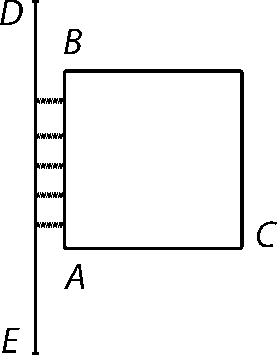
\includegraphics[width=0.51\textwidth]{gesamttex/edit_VIII,3/images/dnr-3a_LH_37_03_071-072_d3a.pdf}
\end{minipage}
\hspace{-1mm}
\begin{minipage}[t][5.8cm][b]{0.33\textwidth}
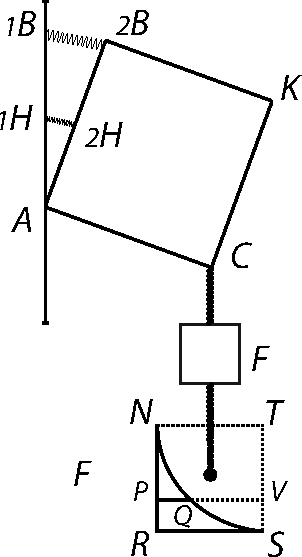
\includegraphics[width=0.69\textwidth]{gesamttex/edit_VIII,3/images/dnr-3b_LH_37_03_071-072_d3b.pdf}
\end{minipage}
\hspace{3mm}
\begin{minipage}[t][5.8cm][b]{0.33\textwidth}
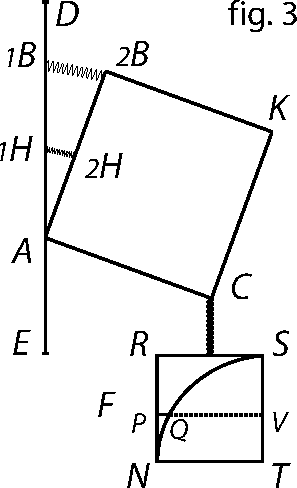
\includegraphics[width=0.69\textwidth]{gesamttex/edit_VIII,3/images/dnr-3c_AE_1684_319-325_d3c.pdf}
\end{minipage}\vspace{1.5em}
\pend\vspace{0.7em}
\pstart
\noindent\setline{1}
\hspace*{2mm} \lbrack\textit{Fig.~3a, gestr.;}\hspace*{19mm} [\textit{Fig.~3b; L\textsuperscript{2}\! (Bl.~72~r\textsuperscript{o}\!)}]\label{AE_1684_321_Fig_3b}\hspace*{19mm} [\textit{Fig.~3c; E\textsuperscript{1}}]\label{AE_1684_321_Fig_3c}
\\
\hspace*{5mm} \textit{L\textsuperscript{2}\,(Bl.~72~r\textsuperscript{o}\!)}\rbrack
\pend
\vspace{-2mm}
\newpage
\count\Bfootins=1100
\count\Afootins=1100
\count\Cfootins=1100
%%
%%
%%
%%  \newpage%
%  \vspace*{-1.0em}%     % Diagramm Fig.~3a
%  \centerline{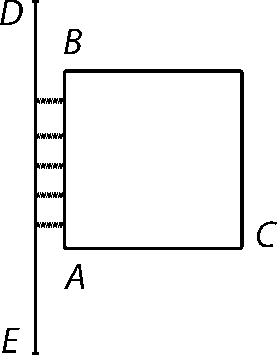
\includegraphics[width=0.16\textwidth]{gesamttex/edit_VIII,3/images/dnr-3a_LH_37_03_071-072_d3a.pdf}}% \hspace*{-100mm}
%  \vspace*{0.5em}
%  \centerline{\lbrack\textit{Fig.~3a, gestr.;}}% \hspace*{-100mm}
%  \centerline{\textit{L\textsuperscript{2}\,(Bl.~72~r\textsuperscript{o}\!)}\rbrack}
%%  \label{}
%%  \newpage%
%%  \vspace*{2.5em}%
%%
%%
%%  \newpage% 
% \vspace{-8.0em}%     % Diagramm Fig.~3b
%  \centerline{\hspace*{-105mm}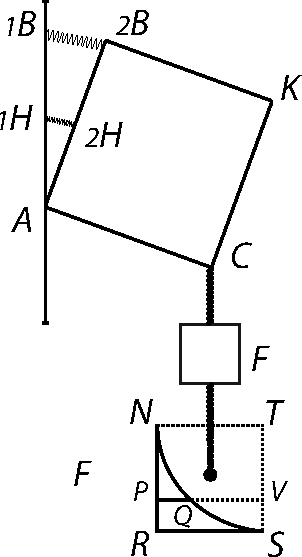
\includegraphics[width=0.24\textwidth]{gesamttex/edit_VIII,3/images/dnr-3b_LH_37_03_071-072_d3b.pdf}}%
%  \vspace*{1.0em}
%  \centerline{\hspace*{-105mm}\lbrack\textit{Fig.~3b; L\textsuperscript{2}\! (Bl.~72~r\textsuperscript{o}\!)}\rbrack}%
%  \label{AE_1684_321_Fig_3b}%
%  \vspace{-1.25em}%
%%  \newpage%
%%
%%
%%  \newpage% 
% \vspace{-16.75em}%     % Diagramm Fig.~3c
%  \centerline{\hspace*{105mm}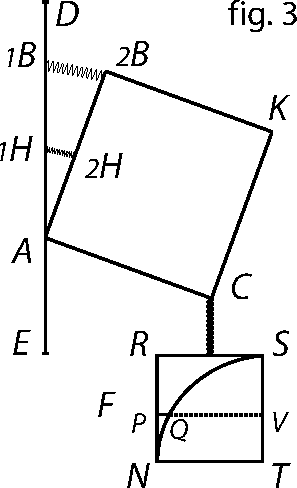
\includegraphics[width=0.24\textwidth]{gesamttex/edit_VIII,3/images/dnr-3c_AE_1684_319-325_d3c.pdf}}%
%  \vspace*{1.0em}
%  \centerline{\hspace*{105mm}\lbrack\textit{Fig.~3c; E\textsuperscript{1}}\rbrack}%
%  \label{AE_1684_321_Fig_3c}%
%%  \vspace{2.0em}%
%  \newpage%
%
%
%Abbildung 4a 4b 4c %%%%%%%%%%%%%%%%%%%%%%%%%%%%%%%%%%%%%%%%
\pstart
\begin{minipage}[t]{0.5\textwidth}
\hspace{9mm}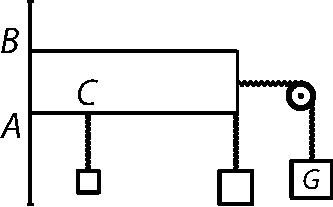
\includegraphics[width=0.45\textwidth]{gesamttex/edit_VIII,3/images/dnr-4a_LH_37_03_071-072_d4a.pdf}
\end{minipage}
\hspace{16mm}
\begin{minipage}[t]{0.5\textwidth}
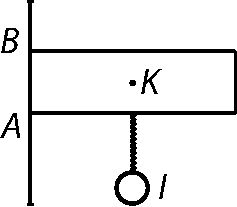
\includegraphics[width=0.32\textwidth]{gesamttex/edit_VIII,3/images/dnr-4b_LH_37_03_071-072_d4b.pdf}
\end{minipage}
\\
\\
\hspace*{8mm} [\textit{Fig.~4a, gestr.; L\textsuperscript{2}\,(Bl.~72~v\textsuperscript{o}\!)}]\label{LH_37_03_072v+AE_1684_323_Fig.4a}\hspace*{24mm} [\textit{Fig.~4b, gestr.; L\textsuperscript{2}\,(Bl.~72~v\textsuperscript{o}\!)}] \label{LH_37_03_072v+AE_1684_323_Fig.4b}%
\phantom{Cfootnote zu Fig.~4:}%
\edtext{}{\lemma{%
\hspace{1,6mm}\lbrack\textit{Fig.~4a}\rbrack\ bis \lbrack\textit{Fig.~4c}\rbrack}%
\killnumber\Cfootnote{%
Kein entsprechendes Diagramm in \textit{L\textsuperscript{1}} überliefert.}}% 
\pend
  \centerline{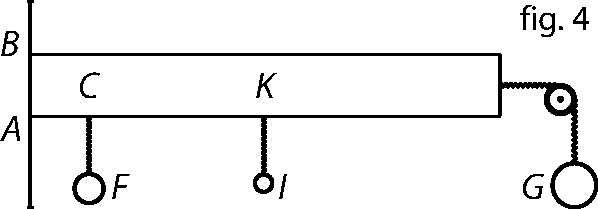
\includegraphics[width=0.48\textwidth]{gesamttex/edit_VIII,3/images/dnr-4c_LH_37_03_071-072+AE_1684_319-325_d4c.pdf}}%\\
  \vspace{0.77em}
  \centerline{\lbrack\textit{Fig.~4c; L\textsuperscript{2} (Bl.~72~v\textsuperscript{o}\!) u. E\textsuperscript{1}}\rbrack}%
  \label{LH_37_03_072v+AE_1684_323_Fig.4c}
\vspace{1.3em}
\count\Bfootins=900
\count\Afootins=900
\count\Cfootins=900
\pstart
\noindent\setline{1}%
pondus\protect\index{Sachverzeichnis}{pondus appensum} \textit{I} appendatur ex \textit{K},
sitque \textit{AK} quadrupla ipsius
\edtext{\textit{AB} vel}{%
\lemma{\textit{AB}}\Bfootnote{%
\hspace{-0,5mm}vel
\textit{erg.~L\textsuperscript{2}}}}
%
\textit{AC},
erit pondus \textit{I} quarta pars ipsius
%
\edtext{\textit{F},}{%
\lemma{\textit{F}~\textit{L\textsuperscript{2}}}\Bfootnote{%
\hspace{0,5mm}\textit{F}~,~\textit{E\textsuperscript{1}}}}
%
et duodecima ipsius \textit{G}.
Generaliter
% <<
\edtext{ergo pondus trabem parallelepipedam\protect\index{Sachverzeichnis}{trabs parallelepipeda}
directe evellens,\protect\index{Sachverzeichnis}{pondus evellens}
erit ad pondus abrumpens transverse\protect\index{Sachverzeichnis}{pondus abrumpens}
seu per modum vectis,\protect\index{Sachverzeichnis}{vectis}
ut longitudo vectis est ad tertiam partem crassitiei trabis.%
\protect\index{Sachverzeichnis}{crassities trabis}}{%
\lemma{ergo}\Bfootnote{\hspace{-0,5mm}%
\textit{(1)}~erit pondus \textit{I} ad pondus \textit{G} in composita ratione ex 3 ad 1 et \textit{AK} ad \textit{AB} seu
\textit{(2)}~pondus
\textit{(a)}~recta
\textit{(b)}~trabem
\textit{(aa)}~directe
\textit{(bb)}~parallelepipedam directe evellens ad pondus abrumpens
\textbar~transverse seu \textit{erg.}~%
\textbar\ per modum vectis erit ut
\textit{(aaa)}~tripla
\textit{(bbb)}~longitudo vectis
\textit{(aaaa)}~ad
\textit{(bbbb)}~est ad tertiam partem crassitiei trabis.%
~\textit{L\textsuperscript{2}}
\hspace{0,5mm}ergo pondus \lbrack...\rbrack\ crassitiei trabis.%
~\textit{E\textsuperscript{1}}}}
% >>
Consideravimus autem hactenus ipsam trabem ut pondere
% <
\edtext{carentem,\protect\index{Sachverzeichnis}{trabs pondere carens}
quod si}{%
\lemma{carentem~;}\Bfootnote{%
\hspace{-0,5mm}quodsi%
~\textit{L\textsuperscript{2}}
\hspace{0,5mm}carentem~, quod si%
~\textit{E\textsuperscript{1}}}}
%
pondus ipsius trabis\protect\index{Sachverzeichnis}{pondus trabis}
in rationes venire debeat,
perinde erit ac si pondus \textit{I} trabi aequale suspensum esset ex
% <
\edtext{\textit{K},}{%
\lemma{\textit{K}~\textit{L\textsuperscript{2}}}\Bfootnote{%
\hspace{0,5mm}\textit{K}~,~\textit{E\textsuperscript{1}}}}
% >
centro gravitatis ipsius trabis.\protect\index{Sachverzeichnis}{centrum gravitatis trabis}
%%
    %%  HIERZU DIE ANMERKUNG VON 1693  !!!!!!
%%
\edlabel{AE_1684_319-325_a3}%
Fieri etiam poterit,
ut trabs\protect\index{Sachverzeichnis}{trabs suo pondere fracta}
pondere suo\protect\index{Sachverzeichnis}{pondus trabis}
frangatur in loco
% <<<
\edtext{aliquo, ut \textit{G} in \,% \textso{ }%
\edtext{\textso{figura}~\textso{5,}}{%
\lemma{\textso{figura}~\textso{5}\,}\Cfootnote{%
Das Diagramm \lbrack\textit{Fig.~5e}\rbrack\ auf S.~\pageref{LH_37_03_072v+AE_1684_323_Fig.5e}.
Ursprünglich bezog sich \textit{L\textsuperscript{2}} jedoch auf das Diagramm \lbrack\textit{Fig.~5b}\rbrack\ ebd.}}}{%
\lemma{aliquo~,}\Bfootnote{\hspace{-0,5mm}%
\textit{(1)}~medio ut 2. 3.
\textit{(2)}~ut \textit{G} in \textso{fig.}~\textso{5}%
~\textit{L\textsuperscript{2}}
\hspace{0,5mm}aliquo~, ut \textit{G} in \textso{figura}~\textso{5,}%
~\textit{E\textsuperscript{1}}}}
% >>>
% <
\edtext{inter\protect\index{Sachverzeichnis}{figura} parietem\protect\index{Sachverzeichnis}{paries} \textit{AB}}{%
\lemma{inter}\Bfootnote{%
\hspace{-0,5mm}murum\protect\index{Sachverzeichnis}{murus}
\textit{(1)}~\textit{AB}
\textit{(2)}~\textit{AB}%
~\textit{L\textsuperscript{2}}
\hspace{0,5mm}inter parietem \textit{AB}%
~\textit{E\textsuperscript{1}}}}
% >
et
\edtext{extremitatem trabis \textit{C},}{%
\lemma{extremitatem}\Bfootnote{%
\textit{(1)}~\textit{X}
\textit{(2)}~trabis \textit{C},%
~\textit{L\textsuperscript{2}}}}
%
quando scilicet gravitatio\protect\index{Sachverzeichnis}{gravitatio trabis}%
\edlabel{KZeitz79}\edtext{}{{\xxref{KZeitz79}{KZeitz80}}%
{%
\lemma{portionis}\Bfootnote{\hspace{-0,5mm}%
\textit{(1)}~\textit{2.3.X} ad resisten
\textit{(2)}~\textit{FGCF} libratae ex
\textit{(a)}~centro $\langle$\textit{F}$\rangle$
\textit{(b)}~puncto quietis \textit{G} majorem habet rationem ad
\textit{(aa)}~resistentiam in
\textit{(bb)}~gravitationem totius \textit{BAX},
\textit{(aaa)}~quam resistentia ex centro \textit{A},
\textit{(bbb)}~quam resistentia in
\textit{(aaaa)}~\textit{2.}
\textit{(bbbb)}~\textit{3.2}
\textit{(cccc)}~\textit{FG}
\textit{(cc)}~resistentiam in % \textit{FG}, quam gravitatio totius trabis \textit{BAC} ex 
\lbrack...\rbrack\ puncto quietis \textit{A}, ad resistentiam in \textit{AB}.%
~\textit{L\textsuperscript{2}}
\hspace{0,5mm}portionis \textit{FGCF}, \lbrack...\rbrack\ \textit{BAC} ex puncto quietis
\textbar~\textit{AD} \textit{ändert Hrsg. nach~L\textsuperscript{2}\! u.\! E\textsuperscript{3}}~%
\textbar~, ad resistentiam in \textit{AB}.%
~\textit{E\textsuperscript{1}}}}}
portionis \makebox[1.0\textwidth][s]{\textit{FGCF}, libratae ex puncto quietis \textit{G},\protect\index{Sachverzeichnis}{punctum quietis}
majorem habet rationem ad resistentiam\protect\index{Sachverzeichnis}{resistentia trabis} in \textit{FG},}
\pend
  \newpage
%% % % % ACHTUNG GETRIXT:
%\pstart%
%\phantom{Cfootnote zu Fig.~4:}%
%%
%% \edtext{}{%
%% \lemma{\hspace{1,6mm}\lbrack\textit{Fig.~3a}\rbrack\ bis \lbrack\textit{Fig.~3c}\rbrack}\killnumber\Cfootnote{%
%% Kein entsprechendes Diagramm ist in \textit{L\textsuperscript{1}} überliefert.
%% \lbrack\textit{Fig.~3c}\rbrack\ ist lediglich in \textit{E\textsuperscript{1}} überliefert.}}%
%%
%\edtext{}{\lemma{%
%\hspace{1,6mm}\lbrack\textit{Fig.~4a}\rbrack\ bis \lbrack\textit{Fig.~4c}\rbrack}%
%\killnumber\Cfootnote{%
%Kein entsprechendes Diagramm in \textit{L\textsuperscript{1}} überliefert.
%% Zu \lbrack\textit{Fig.~4c}\rbrack\ liegt in \textit{L\textsuperscript{2}} ein gestr., nicht wiedergegebener Entwurf vor.
%}}%
%\pend%
%%
%%
%%  \newpage% 
%  \vspace{-0.5em}%     % Diagramm Fig.~4a
%  \centerline{\hspace*{-50mm}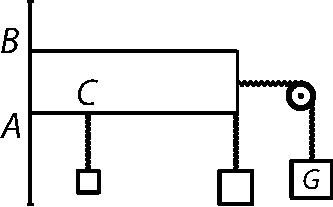
\includegraphics[width=0.20\textwidth]{gesamttex/edit_VIII,3/images/dnr-4a_LH_37_03_071-072_d4a.pdf}}%
%  \vspace*{1.0em}
%  \centerline{\hspace*{-55mm}\lbrack\textit{Fig.~4a, gestr.; L\textsuperscript{2}\,(Bl.~72~v\textsuperscript{o}\!)}\rbrack}%
%  \label{LH_37_03_072v+AE_1684_323_Fig.4a}%
%%  \vspace{2.0em}%
%%  \newpage%
%%
%%
%%  \newpage% 
%  \vspace{-7.25em}%     % Diagramm Fig.~4b
%  \centerline{\hspace*{55mm}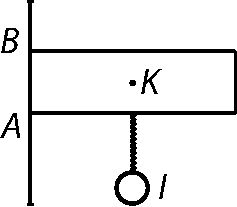
\includegraphics[width=0.14\textwidth]{gesamttex/edit_VIII,3/images/dnr-4b_LH_37_03_071-072_d4b.pdf}}%
%  \vspace*{1.0em}
%  \centerline{\hspace*{60mm}\lbrack\textit{Fig.~4b, gestr.; L\textsuperscript{2}\,(Bl.~72~v\textsuperscript{o}\!)}\rbrack}%
%  \label{LH_37_03_072v+AE_1684_323_Fig.4b}%
%%  \vspace{2em}%
%%  \newpage%
%%
%%
%%  \newpage
%  \vspace{2.0em}%     % Diagramm Fig.~4c
%  \centerline{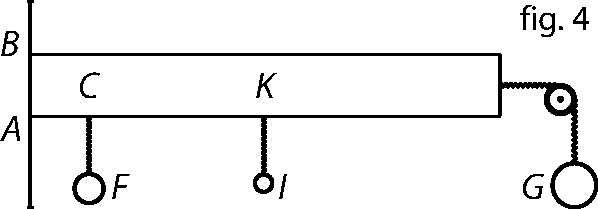
\includegraphics[width=0.48\textwidth]{gesamttex/edit_VIII,3/images/dnr-4c_LH_37_03_071-072+AE_1684_319-325_d4c.pdf}}%\\
%  \vspace*{0.5em}
%  \centerline{\lbrack\textit{Fig.~4c; L\textsuperscript{2} (Bl.~72~v\textsuperscript{o}\!) u. E\textsuperscript{1}}\rbrack}%
%  \label{LH_37_03_072v+AE_1684_323_Fig.4c}
%%  \vspace*{1.0em}
%  \newpage
%%
%%%%%%%%%%%%%%%%%%%%%%%%%%%%%%%%Abbildungen 5a 5b 5c 5d 5e%%%%%%%%%%%%%%%%%%%%%%%%%%
\pstart 
\hspace{8mm}\begin{minipage}[t]{0.5\textwidth}
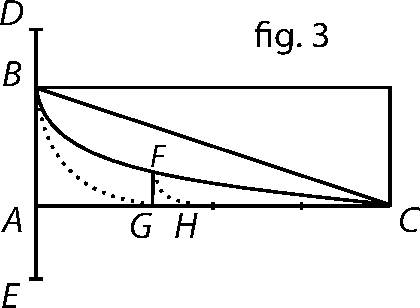
\includegraphics[width=0.49\textwidth]{gesamttex/edit_VIII,3/images/dnr-5a_LH_35_09_16_002-003_d5a.pdf}
\end{minipage}
\hspace{-16mm}
\begin{minipage}[t]{0.5\textwidth}
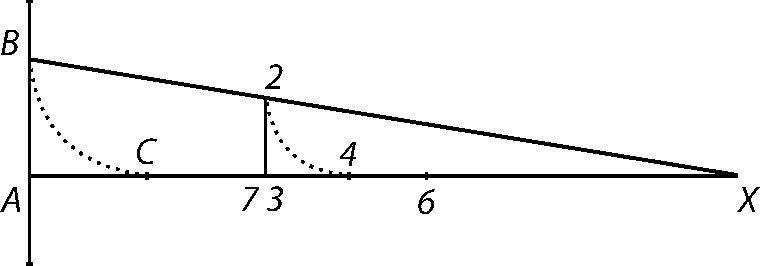
\includegraphics[width=0.9\textwidth]{gesamttex/edit_VIII,3/images/dnr-5b_LH_37_03_071-072_d5b.pdf}
\end{minipage}
\\
\\
\hspace*{9mm} [\textit{Fig.~5a, gestr.; L\textsuperscript{1}\,(Bl.~1~r\textsuperscript{o}\!)}] \label{LH_35_09_16_002r_Fig.5a}\hspace*{20mm} [\textit{Fig.~5b, gestr.; L\textsuperscript{2}\,(Bl.~72~v\textsuperscript{o}\!)}] \label{LH_37_03_072v_Fig.5b}
\pend
\vspace{1em}
\pstart 
\hspace{11mm}\begin{minipage}[t]{0.5\textwidth}
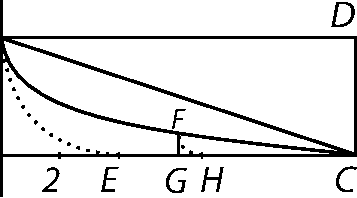
\includegraphics[width=0.41\textwidth]{gesamttex/edit_VIII,3/images/dnr-5c_LH_37_03_071-072_d5c.pdf}
\end{minipage}
\hspace{0mm}
\begin{minipage}[t]{0.5\textwidth}
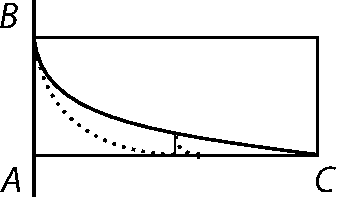
\includegraphics[width=0.41\textwidth]{gesamttex/edit_VIII,3/images/dnr-5d_LH_37_03_071-072_d5d.pdf}
\end{minipage}
\\
\\
\hspace*{9mm} [\textit{Fig.~5c, gestr.; L\textsuperscript{2}\,(Bl.~72~v\textsuperscript{o}\!)}] \label{LH_37_03_072v_Fig.5c}\hspace*{19mm} [\textit{Fig.~5d, gestr.; L\textsuperscript{2}\,(Bl.~72~v\textsuperscript{o}\!)}]\label{LH_37_03_072v_Fig.5d}
\pend
\vspace{1em}
 \centerline{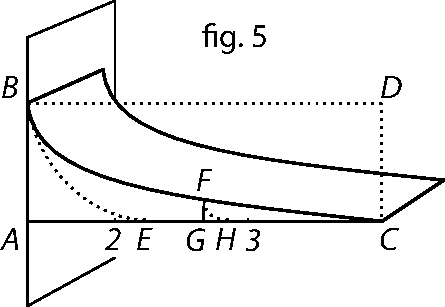
\includegraphics[width=0.39\textwidth]{gesamttex/edit_VIII,3/images/dnr-5e_LH_37_03_071-072+AE_1684_319-325_d5e.pdf}}%\\
%  \vspace*{0.5em}
\setline{1}\centerline{\lbrack\textit{Fig.~5e; L\textsuperscript{2}\,(Bl.~72~v\textsuperscript{o}\!) u. E\textsuperscript{1}}\rbrack}%
  \label{LH_37_03_072v+AE_1684_323_Fig.5e}%
%  \vspace*{3.0em}
%  \newpage%
%
%
\vspace{-4mm}
\pstart%
\phantom{Cfootnote zu den Diagrammen Fig. 5a bis Fig. 5e}%
%
\edtext{}{\lemma{\hspace{1,6mm}\lbrack\textit{Fig.~5a}\rbrack}%
\killnumber\Cfootnote{%
Hierauf war ursprünglich die Passage \textit{Est enim} \lbrack...\rbrack\ \textit{dare possum} (S.~\refpassage{AE_1684_323-324_erstzng-1}{AE_1684_323-324_erstzng-2}) in \textit{L\textsuperscript{1}} % \,(Bl.~2~r\textsuperscript{o}) 
bezogen. Der Buchstabe \textit{D} bezeichnete anfangs den Eckpunkt über \textit{C}.}}%
%
\edtext{}{\lemma{\hspace{1,6mm}\lbrack\textit{Fig.~5b}\rbrack}%
\killnumber\Cfootnote{%
Hierauf war \textit{L\textsuperscript{2}} ur\-sprünglich bezogen, etwa in der gestr. Passage S.~\refpassage{LH_37_03_072v_erstzng-1}{LH_37_03_072v_erstzng-2}.}}%
%
\edtext{}{\lemma{\hspace{1,6mm}\lbrack\textit{Fig.~5c}\rbrack\ und \lbrack\textit{Fig.~5d}\rbrack}%
\killnumber\Cfootnote{%
Entwürfe zu \lbrack\textit{Fig.~5e}\rbrack.}}%
%
\edtext{}{\lemma{\hspace{1,6mm}\lbrack\textit{Fig.~5e}\rbrack}%
\killnumber\Cfootnote{%
Hierauf nehmen die überarbeitete Passage \textit{Est enim} \lbrack...\rbrack\ \textit{dare possum} (S.~\refpassage{AE_1684_323-324_erstzng-1}{AE_1684_323-324_erstzng-2}) in \textit{L\textsuperscript{1}} sowie die überarbeitete Fassung von \textit{L\textsuperscript{2}} Bezug.}}%
\pend%
%\newpage
%%
%%
%%  \newpage% 
% \vspace*{0.0em}%     % Diagramm Fig.~5a
%  \centerline{\hspace*{-85mm}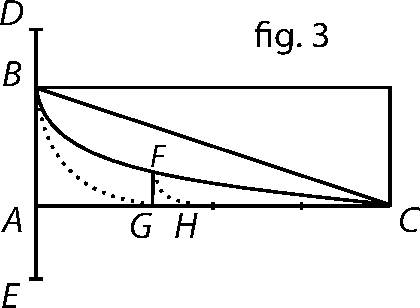
\includegraphics[width=0.24\textwidth]{gesamttex/edit_VIII,3/images/dnr-5a_LH_35_09_16_002-003_d5a.pdf}}%
%  \vspace*{1.0em}
%  \centerline{\hspace*{-85mm}\lbrack\textit{Fig.~5a, gestr.; L\textsuperscript{1}\,(Bl.~1~r\textsuperscript{o}\!)}\rbrack}%
%  \label{LH_35_09_16_002r_Fig.5a}%
%%  \vspace{2.0em}%
%%  \newpage%
%%
%%
%%  \newpage
%  \vspace{-8.25em}%     % Diagramm Fig.~5b
%  \centerline{\hspace*{75mm}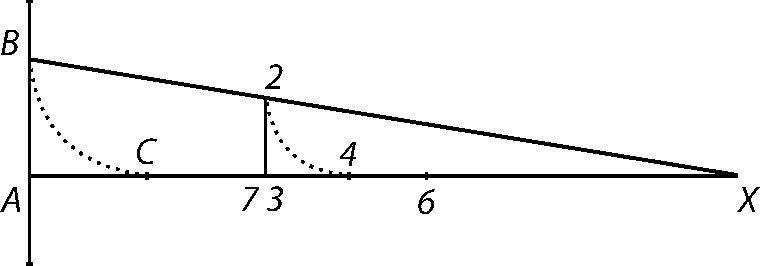
\includegraphics[width=0.44\textwidth]{gesamttex/edit_VIII,3/images/dnr-5b_LH_37_03_071-072_d5b.pdf}}%
%  \vspace*{0.5em}
%  \centerline{\hspace*{75mm}\lbrack\textit{Fig.~5b, gestr.; L\textsuperscript{2}\,(Bl.~72~v\textsuperscript{o}\!)}\rbrack}%
%  \label{LH_37_03_072v_Fig.5b}
%%  \vspace*{2.5em}
%%  \newpage
%%
%%
%%  \newpage% 
% \vspace{3.25em}%     % Diagramm Fig.~5c
%  \centerline{\hspace*{-75mm}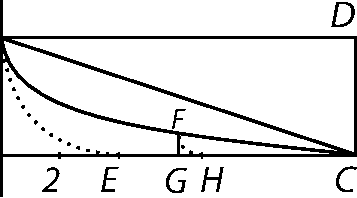
\includegraphics[width=0.20\textwidth]{gesamttex/edit_VIII,3/images/dnr-5c_LH_37_03_071-072_d5c.pdf}}%
%  \vspace*{1.0em}
%  \centerline{\hspace*{-75mm}\lbrack\textit{Fig.~5c, gestr.; L\textsuperscript{2}\,(Bl.~72~v\textsuperscript{o}\!)}\rbrack}%
%  \label{LH_37_03_072v_Fig.5c}%
%%  \vspace{2em}%
%%  \newpage%
%%
%%
%%  \newpage%
% \vspace{-7.25em}%     % Diagramm Fig.~5d
%  \centerline{\hspace*{75mm}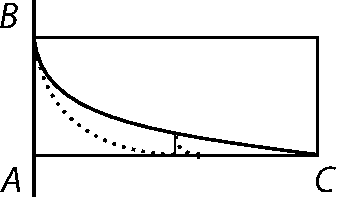
\includegraphics[width=0.20\textwidth]{gesamttex/edit_VIII,3/images/dnr-5d_LH_37_03_071-072_d5d.pdf}}%
%  \vspace*{1.0em}
%  \centerline{\hspace*{75mm}\lbrack\textit{Fig.~5d, gestr.; L\textsuperscript{2}\,(Bl.~72~v\textsuperscript{o}\!)}\rbrack}%
%  \label{LH_37_03_072v_Fig.5d}%
%%  \vspace{2em}%
%%  \newpage%
%%
%%
%  \vspace{3.25em}%     % Diagramm Fig.~5e
%  \centerline{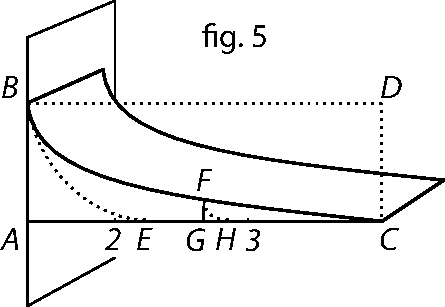
\includegraphics[width=0.40\textwidth]{gesamttex/edit_VIII,3/images/dnr-5e_LH_37_03_071-072+AE_1684_319-325_d5e.pdf}}%\\
%%  \vspace*{0.5em}
%  \centerline{\lbrack\textit{Fig.~5e; L\textsuperscript{2}\,(Bl.~72~v\textsuperscript{o}\!) u. E\textsuperscript{1}}\rbrack}%
%  \label{LH_37_03_072v+AE_1684_323_Fig.5e}
%%  \vspace*{3.0em}
%%  \newpage%
%%
%%
%\pstart%
%\phantom{Cfootnote zu den Diagrammen Fig. 5a bis Fig. 5e}%
%%
%\edtext{}{\lemma{\hspace{1,6mm}\lbrack\textit{Fig.~5a}\rbrack}%
%\killnumber\Cfootnote{%
%Hierauf war ursprünglich die Passage \textit{Est enim} \lbrack...\rbrack\ \textit{dare possum} (S.~\refpassage{AE_1684_323-324_erstzng-1}{AE_1684_323-324_erstzng-2}) in \textit{L\textsuperscript{1}} % \,(Bl.~2~r\textsuperscript{o}) 
%bezogen. Der Buchstabe \textit{D} bezeichnete anfangs den Eckpunkt über \textit{C}.}}%
%%
%\edtext{}{\lemma{\hspace{1,6mm}\lbrack\textit{Fig.~5b}\rbrack}%
%\killnumber\Cfootnote{%
%Hierauf war \textit{L\textsuperscript{2}} ursprünglich bezogen, etwa in der gestr. Passage S.~\refpassage{LH_37_03_072v_erstzng-1}{LH_37_03_072v_erstzng-2}.}}%
%%
%\edtext{}{\lemma{\hspace{1,6mm}\lbrack\textit{Fig.~5c}\rbrack\ und \lbrack\textit{Fig.~5d}\rbrack}%
%\killnumber\Cfootnote{%
%Entwürfe zu \lbrack\textit{Fig.~5e}\rbrack.}}%
%%
%\edtext{}{\lemma{\hspace{1,6mm}\lbrack\textit{Fig.~5e}\rbrack}%
%\killnumber\Cfootnote{%
%Hierauf nehmen die überarbeitete Passage \textit{Est enim} \lbrack...\rbrack\ \textit{dare possum} (S.~\refpassage{AE_1684_323-324_erstzng-1}{AE_1684_323-324_erstzng-2}) in \textit{L\textsuperscript{1}} sowie die überarbeitete Fassung von \textit{L\textsuperscript{2}} Bezug.}}
%\pend%
%\newpage%
%%
%%
%%
%%
\count\Bfootins=900
\count\Afootins=900
\count\Cfootins=900
\pstart
\noindent\setline{1}%
% >>
quam gravitatio totius trabis \textit{BAC}\protect\index{Sachverzeichnis}{gravitatio trabis}
ex puncto quietis \lbrack\textit{A}\rbrack,\protect\index{Sachverzeichnis}{punctum quietis}
ad resistentiam\protect\index{Sachverzeichnis}{resistentia trabis} in \textit{AB}.\edlabel{KZeitz80}
% >>>
% <<<
\edtext{Quaeritur\edlabel{LH_37_03_072v_L2-trabstriangularis} autem,
qualis esse debeat
% <
\edtext{linea \textit{BFC},}{%
\lemma{linea}\Bfootnote{\hspace{-0,5mm}%
\textit{(1)}~\textit{B}
\textit{(2)}~\textit{2X},
\textit{(3)}~\textit{BFC},%
~\textit{L\textsuperscript{2}}}}
% >
ut resistentiae\protect\index{Sachverzeichnis}{resistentia trabis} sint
% <
\edtext{gravitationibus respondentibus proportionales,\protect\index{Sachverzeichnis}{gravitatio trabis}
et trabs ubique aequaliter resistat:\protect\index{Sachverzeichnis}{trabs aequiresistens}}{%
\lemma{gravitationibus}\Bfootnote{\hspace{-0,5mm}%
\textbar~respondentibus \textit{erg.}~%
\textbar\ proportionales
\textbar~et trabs ubique aequaliter resistat \textit{erg.}~\textbar%
~\textit{L\textsuperscript{2}}
\hspace{0,5mm}gravitationibus respondentibus \lbrack...\rbrack\ aequaliter resistat:%
~\textit{E\textsuperscript{1}}}}%
% >
}{\lemma{Quaeritur \lbrack...\rbrack\ resistat}\Cfootnote{%
Diese Frage war zunächst von Galilei\protect\index{Namensregister}{\textso{Galilei} (Galilaeus, Galileus), Galileo 1564\textendash1642}
% mit ähnlichen Ergebnissen wie in \textit{E\textsuperscript{1}}, 
behandelt worden;
vgl. \textit{Discorsi}, S.~137\textendash141\cite{00050} (\textit{GO} VIII,\cite{00048} S.~177\textendash181). % S.~177.29\textendash181.15 184.15 \textsc{}, 
Leibniz hatte sich damit in Paris befasst; siehe \textit{LSB} VIII,~2 N.~22.\cite{01252}
Siehe zudem N.~14\textsubscript{4} und 14\textsubscript{8} in diesem Band.}}
% >>>
hanc ergo %
%
\pend%
\newpage% % % % %    REIN VORLÄUFIG 
%\vspace*{0.5em}%
%%
%%
    %%%%    %%%%    HIER BEGINNT DER ABWEICHENDE TEXT    %%%%    %%%%
%%
%%
\pstart%
\noindent%
\lbrack%
\textit{Nachfolgend kleingedruckter Text in L\textsuperscript{2}\,(Bl.~72~v\textsuperscript{o}\!) gestrichen%
% und in \textit{E\textsuperscript{1}} durch den % von L\textsuperscript{1} stammenden 
% Text\-abschnitt} Est enim ... dare possum \textit{(S.~\refpassage{AE_1684_323-324_erstzng-1}{AE_1684_323-324_erstzng-2}) ersetzt
:}\rbrack%
\pend%
\footnotesize%
\vspace{0.5em}%
% \newpage%
%
\pstart%
\noindent%
\footnotesize%
comperi\edlabel{LH_37_03_072v_erstzng-1}%
\edtext{}{%
{\xxref{LH_37_03_072v_erstzng-1}{LH_37_03_072v_erstzng-2}}%
{\lemma{comperi \lbrack...\rbrack\ desiderabatur}\Cfootnote{%
Die gestr. Passage gehört zur ältesten Fassung von \textit{L\textsuperscript{2}}
(siehe zur Entstehung von N.~14\textsubscript{6} die editorische Vorbemerkung, S.~\refpassage{DNDRS_Ueberarbeitung_scjvtx-1}{DNDRS_Ueberarbeitung_scjvtx-2}).
Einen ähnlichen Gedanken wie hier hat Leibniz im Konzept \textit{L\textsuperscript{2}} seines Briefes an Mariotte von März/April 1683 geäußert und dann ebenfalls getilgt; vgl. \cite{01262}\textit{LSB} III,~4 N.~456, S.~796.9\textendash32.}}}
% \edtext{}{%
% {\xxref{LH_37_03_072v_erstzng-1}{LH_37_03_072v_erstzng-2}}%
% {\lemma{comperi}\Bfootnote{%
% \hspace{-0,5mm}esse \lbrack...\rbrack\ Quod desiderabatur.
% \textit{fehlt~E\textsuperscript{1}}}}
%
esse rectam,
seu trabem\protect\index{Sachverzeichnis}{trabs prismatica}
\edtext{debere esse prisma triangulare.\protect\index{Sachverzeichnis}{prisma triangulare}}{%
\lemma{debere}\Bfootnote{%
\hspace{-0,5mm}esse
\textit{(1)}~triangularem
\textit{(2)}~prisma triangulare.%
~\textit{L\textsuperscript{2}}}}
%
\edtext{Cujus sectio\protect\index{Sachverzeichnis}{sectio trabis} quaelibet
perpendicularis ad horizontem\protect\index{Sachverzeichnis}{horizon} et murum\protect\index{Sachverzeichnis}{murus}
sit
\edtext{triangulum\protect\index{Sachverzeichnis}{triangulum} \textit{ABX}}{%
\lemma{triangulum \textit{ABX}}\Cfootnote{%
Siehe das Diagramm \lbrack\textit{Fig.~5b}\rbrack\ auf S.~\pageref{LH_37_03_072v_Fig.5b}.}}
habens basin}{%
\lemma{Cujus}\Bfootnote{%
\textit{(1)}~trianguli
\textit{(a)}~bas
\textit{(b)}~\textit{A}
\textit{(2)}~sectio sit triangulum
\textit{(3)}~sectio verticalis
\textit{(4)}~sectio
\textbar~quaelibet \textit{erg.}~%
\textbar\ perpendicularis ad \lbrack...\rbrack\ habens basin%
~\textit{L\textsuperscript{2}}}}
%
in muro,\protect\index{Sachverzeichnis}{murus}
apicem in extremitate trabis;
eamque trabem ita formatam,\protect\index{Sachverzeichnis}{trabs aequiresistens}
\edtext{ajo}{%
\lemma{ajo}\Bfootnote{\textit{erg.~L\textsuperscript{2}}}}
%
ubique aequaliter ponderi suo\protect\index{Sachverzeichnis}{pondus trabis}
\edtext{resistere.
Quod ut ostendam,}{%
\lemma{resistere.}\Bfootnote{%
\textit{(1)}~Quod
\textit{(a)}~\textit{2.3} sit a
\textit{(b)}~\textit{BA} sit a
\textit{(2)}~Quod ut ostendam,%
~\textit{L\textsuperscript{2}}}}
%
sit \textit{3.6} pars tertia ipsius \textit{3.X}
et \textit{A.7} pars tertia ipsius \textit{AX},
erit \textit{3.6} distantia centri gravitatis\protect\index{Sachverzeichnis}{centrum gravitatis trabis}
trianguli\protect\index{Sachverzeichnis}{triangulum} \textit{2.3.X} a recta \textit{2.3},
et \textit{A.7} distantia centri gravitatis
trianguli \textit{BAX} a recta
\edtext{\textit{BA}.
Est autem gravitatio\protect\index{Sachverzeichnis}{gravitatio trabis}}{%
\lemma{\textit{BA}}\Bfootnote{%
\textit{(1)}~eritque gravitatio
\textit{(2)}~. Est autem gravitatio%
~\textit{L\textsuperscript{2}}}}
%
seu momentum\protect\index{Sachverzeichnis}{momentum trabis}
\edtext{figurae\protect\index{Sachverzeichnis}{figura} ut}{%
\lemma{figurae}\Bfootnote{%
\textit{(1)}~idem quod
\textit{(2)}~ut%
~\textit{L\textsuperscript{2}}}}
%
factum ex ductu areae in distantiam centri gravitatis;\protect\index{Sachverzeichnis}{centrum gravitatis trabis}
ergo momenta
% <
\edtext{triangulorum praedicta,}{%
\lemma{triangulorum}\Bfootnote{%
\hspace{-0,5mm}\textbar~prae \textit{erg.}
\textbar\ dicta,%
~\textit{L\textsuperscript{2}}}}
% >
erunt in composita ratione triangulorum ipsorum et distantiarum,
sunt autem triangula\protect\index{Sachverzeichnis}{triangulum}
\edtext{\textit{2.3.X} et}{%
\lemma{\textit{2.3.X}}\Bfootnote{%
\textit{(1)}~ad
\textit{(2)}~et%
~\textit{L\textsuperscript{2}}}}
%
\textit{BAX},
ut quadrata\protect\index{Sachverzeichnis}{quadratum}
\edtext{rectarum \textit{2.3} et \textit{BA}\lbrack,\rbrack\ et}{%
\lemma{rectarum}\Bfootnote{%
\textit{(1)}~\textit{BA} et
\textit{(2)}~\textit{2.3} et \textit{BA} et%
~\textit{L\textsuperscript{2}}}}
%
distantiae
\edtext{\textit{3.6} et}{%
\lemma{\textit{3.6}}\Bfootnote{%
\textit{(1)}~ad
\textit{(2)}~et%
~\textit{L\textsuperscript{2}}}}
%
\textit{A.7}
\edtext{sunt ut rectae \textit{3.X} et \textit{AX}}{%
\lemma{sunt}\Bfootnote{% \hspace{-0,5mm}
ut
\textit{(1)}~triplae earum
\textit{(2)}~rectae
\textit{(a)}~\textit{AX} et
\textit{(b)}~\textit{3.X} et \textit{AX}
%
~\textit{L\textsuperscript{2}}}}
%
\edtext{seu ut \textit{2.3} et \textit{BA}.
Ergo}{%
\lemma{seu}\Bfootnote{% \hspace{-0,5mm}
ut
\textit{(1)}~\textit{2.3} ad \textit{BA}; ergo
\textit{(2)}~\textit{2.3} et \textit{BA}. Ergo%
~\textit{L\textsuperscript{2}}}}
%
composita ratio
\edtext{triangulorum
(\protect\vphantom)%
quae sunt in duplicata%
\protect\vphantom()
et distantiarum
(\protect\vphantom)%
quae sunt in simplici ratione rectarum \textit{2.3} et \textit{BA}%
\protect\vphantom()}{%
\lemma{triangulorum}\Bfootnote{%
\textit{(1)}~et distantiarum, seu quadratorum \textit{2.3} et \textit{BA}, ipsarumque rectarum \textit{2.3} et \textit{BA},
\textit{(2)}~(\protect\vphantom)quae sunt in duplicata
\textit{(a)}~ratione,
\textit{(b)}~\protect\vphantom() et distantiarum \lbrack...\rbrack\ \textit{2.3} et \textit{BA}\protect\vphantom()% 
% (\protect\vphantom)quae sunt in simplici ratione rectarum
~\textit{L\textsuperscript{2}}}}
%
erit triplicata rectarum \textit{2.3} et \textit{BA},
seu momentum trianguli
\edtext{\lbrack\textit{2.3.X}\rbrack}{%
\lemma{\textit{2BX}}\Bfootnote{\textit{L\textsuperscript{2}~ändert Hrsg.}}}
ex \textit{3} gravitantis,
erit ad momentum trianguli \textit{BAX} ex \textit{A} gravitantis,
ut\protect\index{Sachverzeichnis}{cubus}
% <<
\edtext{cubus ipsius \textit{2.3}
ad cubum ipsius \textit{BA.}}{%
\lemma{cubus}\Bfootnote{\hspace{-0,5mm}%
\textit{(1)}~\textit{2.3}
\textit{(2)}~ipsius \textit{2.3} ad cubum ipsius
\textit{(a)}~\textit{AB.}
\textit{(b)}~\textit{BA.}%
~\textit{L\textsuperscript{2}}}}
% >>
\pend%
\count\Bfootins=1000
\count\Afootins=1000
\count\Cfootins=1000
\pstart%
% \footnotesize%
Sed resistentiae\protect\index{Sachverzeichnis}{resistentia trabis} in \textit{2.3} et \textit{BA} sunt inter se
\edtext{ut trilinea}{%
\lemma{ut}\Bfootnote{%
\textit{(1)}~spatia
\textit{(2)}~trilinea%
~\textit{L\textsuperscript{2}}}}
%
parabolica\protect\index{Sachverzeichnis}{trilineum parabolicum} concava \textit{2.3.4.2} et \textit{BACB}
basin et altitudinem aequalem habentia
\edtext{per antedicta}{%
{\lemma{per}\Bfootnote{%
\hspace{-0,5mm}antedicta
\textit{erg.~L\textsuperscript{2}}}%
{\lemma{per antedicta}\Cfootnote{%
Siehe S.~\refpassage{LH_37_03_072r+AE_1684_322-1}{LH_37_03_072r+AE_1684_322-2}.}}}}%
\lbrack,\rbrack\
%
quae
% <<
\edtext{sunt etiam inter se
ut cubi\protect\index{Sachverzeichnis}{cubus}
altitudinum \textit{2.3} et \textit{BA}}{%
\lemma{sunt}\Bfootnote{%
\textit{(1)}~ut cu
\textit{(2)}~etiam inter \lbrack...\rbrack\ cubi altitudinum % se ut
\textit{(a)}~, seu ut cubi
\textit{(b)}~\textit{2.3} et \textit{BA}%
~\textit{L\textsuperscript{2}}}}%
\lbrack,\rbrack\
% >>
ergo momenta\protect\index{Sachverzeichnis}{momentum trabis}
sunt resistentiis\protect\index{Sachverzeichnis}{resistentia trabis}
\edtext{proportionalia.
Itaque cum momentum prius sit ad posterius ut resistentia prior ad posteriorem,
erit et momentum prius ad resistentiam priorem,
ut momentum\protect\index{Sachverzeichnis}{momentum trabis} posterius
ad resistentiam\protect\index{Sachverzeichnis}{resistentia trabis} posteriorem,
ac proinde aequalis ubique trabis firmitas erit.\protect\index{Sachverzeichnis}{firmitas trabis}
Quod desiderabatur.\edlabel{LH_37_03_072v_erstzng-2}}{%
\lemma{proportionalia}\Bfootnote{%
\textit{(1)}~, quod desiderabatur
\textit{(2)}~. Itaque
\textit{(a)}~erit
\textit{(b)}~cum momentum
\textit{(aa)}~unu
\textit{(bb)}~prius
\textbar~sit \textit{erg.}~%
\textbar\ ad posterius \lbrack...\rbrack\ ac proinde
\textit{(aaa)}~aequaliter ubique resistetur
\textit{(bbb)}~aequalis ubique trabis firmitas erit.
\textit{(aaaa)}~Et si
\textit{(bbbb)}~Quod desiderabatur.%
~\textit{L\textsuperscript{2}}}}%
%
\pend%
\normalsize
\newpage
\pstart%
\noindent%
invenietur%
\edlabel{AE_1684_323-324_erstzng-1}%
\edlabel{LH_37_03_071-072+AE_1684_319-325_L1omissa_rjsuv-2}
esse Parabolicam.\protect\index{Sachverzeichnis}{linea parabolica}%
\edlabel{LH_37_03_071-072+AE_1684_319-325_invenieturparabolicam}%
\edtext{}{{%
{\xxref{AE_1684_323-324_erstzng-1}{LH_37_03_071-072+AE_1684_319-325_invenieturparabolicam}}
{\lemma{invenietur}\Bfootnote{\hspace{-0,5mm}%
\textit{(1)}~secundum nostram proportionem adhuc manere Parabolicam ut in \textso{fig.}~\textso{3.} Nam
\textit{(a)}~res fa
\textit{(b)}~sumendo \textit{AG} aequ. \textit{AB}, et \textit{GH} aequal. \textit{GF} 
\textit{(aa)}~patet
\textit{(aaa)}~resistentiam in \textit{GF} fore ad resistentiam in \textit{AB} ut trili
% \textit{(aaaa)}~\textit{GF}
% \textit{(bbbb)}~\textit{2.3} sit
% \textit{(cccc)}~\textit{BA} sit
\textit{(bbb)}~resistentias
\textit{(bb)}~patet resistentias in \textit{GF} et in \textit{AB} fore inter se ut
\textit{(aaa)}~trili
\textit{(bbb)}~linea parabolica concava \textit{FGHF}, \textit{ABGA} seu ut
\textit{(aaaa)}~rectangula circumscripta\protect\index{Sachverzeichnis}{rectangulum circumscriptum}
\textit{(bbbb)}~eorum tripla nempe rectangula circumscripta quae sunt 
\textit{(aaaaa)}~quadrata
\textit{(bbbbb)}~nihil aliud quam quadrata rectarum \textit{GF}, \textit{AB}. Ergo resistentiae sunt ut
\textit{(aaaaa-a)}~quadrata
\textit{(bbbbb-b)}~haec quadrata, prorsus ut supra.
\textit{(2)}~esse Parabolicam.%
~\textit{L\textsuperscript{2}}
% \hspace{0,5mm}invenietur esse Parabolicam.% Est enim \lbrack...\rbrack\ dare possum.% ~\textit{E\textsuperscript{1}}
}}}%
{{\lemma{invenietur esse Parabolicam}\Cfootnote{%
Ersetzt in \textit{L\textsuperscript{2}} die dort gestrichene Passage \textit{comperi esse} \lbrack...\rbrack\ \textit{Quod desiderabatur} (S.~\refpassage{LH_37_03_072v_erstzng-1}{LH_37_03_072v_erstzng-2}).
Beide Textvarianten\,\textit{(1)} und\,\textit{(2)} gehören somit zur bearbeiteten Fassung von \textit{L\textsuperscript{2}}
(siehe zur Entstehung von N.~14\textsubscript{6} die editorische Vorbemerkung, S.~\refpassage{DNDRS_Ueberarbeitung_scjvtx-1}{DNDRS_Ueberarbeitung_scjvtx-2}).
Die in der Variante\,\textit{(1)} % von \textit{L\textsuperscript{2}} 
erwähnte \textit{fig.~3} ist das Diagramm \lbrack\textit{Fig.~5e}\rbrack\ auf S.~\pageref{LH_37_03_072v+AE_1684_323_Fig.5e}.
Der Verweis \textit{ut supra} bezieht sich auf S.~\refpassage{LH_37_03_072r+AE_1684_322-1}{LH_37_03_072r+AE_1684_322-2}}}}}%
%
% % % %   HIER BEGINNT DIE MARGINALIE MIT VERWEIS AUF SONNE & MONDE
\label{LH_37_03_072r-SonneMonde}%
\edtext{}{\lemma{\textit{In L\textsuperscript{2} am Rand von Bl.~72~v\textsuperscript{o}\!,}}\Afootnote{%
\hspace{-0,5mm}\textit{mit einem auf} Parabolicam \textit{bezogenen Einfügungszeichen:}
Inseratur hic quicquid ascriptum ad pag. $\Sun$\textsuperscript{\lbrack a\rbrack} de ($\rightmoon$) usque ad ($\rightmoon$).%
\newline%
\newline%
\footnotesize{%
\textsuperscript{\lbrack a\rbrack} pag. $\Sun$\,:
Der Abschnitt \textit{Est enim} \lbrack...\rbrack\ \textit{dare possum}
(S.~\refpassage{AE_1684_323-324_erstzng-1}{AE_1684_323-324_erstzng-2})
ist nicht in \textit{L\textsuperscript{2}} überliefert,
\mbox{wohl} aber \textendash\ mit Ausnahme der letzten Zeile \textendash\
in \textit{L\textsuperscript{1}} (Bl.~2~r\textsuperscript{o}\!), % N.~??Y\textsubscript{7}, S.~\refpassage{LH_35_09_16_002_Mond-1}{LH_35_09_16_002_Mond-2}% \refpassage{AE_1684_323-324_erstzng-3}{AE_1684_323-324_erstzng-4} 
wo er tatsächlich von zwei Mondsichelzeichen ($\rightmoon$) eingeschlossen ist;
dort % (am Kopf von Bl.~2~r\textsuperscript{o}\!) 
ist am Blattkopf auch ein Sonnenzeichen $\astrosun$ vermerkt.
Der ganze Abschnitt ist, wie \textit{L\textsuperscript{1}} insgesamt, gestrichen.%
}}}%
% % % %   HIER ENDET DIE MARGINALIE MIT VERWEIS AUF SONNE & MONDE
\edtext{}{%
{\xxref{AE_1684_323-324_erstzng-1}{AE_1684_323-324_erstzng-2}}%
{\lemma{Est}\Bfootnote{%
\hspace{-0,5mm}enim \lbrack...\rbrack\ dare possum.
\textit{fehlt~L\textsuperscript{2}}}}}%
%
\edlabel{dnrs_AE_1684_323-324_estenim_jrh-1}%
Est enim resistentia\protect\index{Sachverzeichnis}{resistentia trabis}
\edtext{in \textit{FG}}{%
\lemma{in \textit{FG}}\Cfootnote{%
Siehe % das Diagramm 
\lbrack\textit{Fig.~5e}\rbrack\ auf S.~\pageref{LH_37_03_072v+AE_1684_323_Fig.5e}.}}
%
ad resistentiam in \textit{BA}\protect\index{Sachverzeichnis}{trilineum parabolicum}
% <<<
\edtext{ut trilineum parabolicum concavum \textit{FGHF} ad aliud \textit{BAEB},
si basis trilinei sit altitudini ejusdem aequalis,
(\protect\vphantom)%
ut patet
\edtext{ex praecedentibus:}{%
\lemma{ex praecedentibus}\Cfootnote{%
Siehe S.~\refpassage{LH_37_03_072r+AE_1684_322-1}{LH_37_03_072r+AE_1684_322-2}.}}%
\protect\vphantom() seu}{%
\lemma{ut}\Bfootnote{\hspace{-0,5mm}%
\textit{(1)}~triangulum cujus altitudo et basis
\textbar~aequalis est ipsi \textit{erg.}~\textbar\ \textit{FG} ad triangulum simile cujus altitudo et basis
\textit{(a)}~\textit{BA}, quae
\textit{(b)}~aequalis ipsi \textit{BA} ergo
\textit{(2)}~trilineum parabolicum concavum \textit{FGHF} ad
\textit{(a)}~aliud trilineum
\textit{(b)}~aliud \textit{BAEB}, \lbrack...\rbrack\ aequalis, ut patet ex praecedentibus seu% ejusdem
~\textit{L\textsuperscript{1}}
\hspace{0,5mm}ut trilineum \lbrack...\rbrack\ praecedentibus:\protect\vphantom() seu%
~\textit{E\textsuperscript{1}}}}
% >>>
ut quadratum \textit{FG} ad quadratum\protect\index{Sachverzeichnis}{quadratum}
% <<
\edtext{\textit{BA} (\protect\vphantom)%
quia trilineum tale\protect\index{Sachverzeichnis}{trilineum parabolicum}
est tertia pars quadrati circumscripti.\protect\index{Sachverzeichnis}{quadratum circumscriptum}%
\protect\vphantom()\edlabel{AE_1684_319-325_a4}
% \edtext{}{\lemma{}\Afootnote{\textit{Hierzu Kommentar von Leibniz in Marginalie zu S. \refpassage{AE_1684_319-325_a3}{AE_1684_319-325_a4}}}}
Sed}{%
\lemma{\textit{BA}}\Bfootnote{\hspace{-0,5mm}%
\textbar~quia trilineum \lbrack...\rbrack\ quadrati circumscripti; \textit{erg.}~%
\textbar\ sed%
\textit{~L\textsuperscript{1}}
\hspace{0,5mm}\textit{BA} (\protect\vphantom)quia
\lbrack...\rbrack\ circumscripti.\protect\vphantom() Sed%
~\textit{E\textsuperscript{1}}}}
% >>
momentum\protect\index{Sachverzeichnis}{momentum trabis}
% <
\edtext{seu gravitatio\protect\index{Sachverzeichnis}{gravitatio trabis}}{%
\lemma{seu}\Bfootnote{%
\hspace{-0,5mm}gravitatio
\textit{erg.~L\textsuperscript{1}}}}
% >
% <<
\edtext{portionis \textit{FGCF} cujuscunque ex \textit{G} libratae,}{%
\lemma{portionis}\Bfootnote{\hspace{-0,5mm}%
\textit{(1)}~\textit{CF}
\textit{(2)}~\textit{FGCF} cujuscunque ex
\textit{(a)}~\textit{F}
\textit{(b)}~\textit{G}
\textit{(aa)}~librata
\textit{(bb)}~libratae%
~\textit{L\textsuperscript{1}}
\hspace{0,5mm}portionis \textit{FGCF} \lbrack...\rbrack\ \textit{G} libratae,% cujuscunque ex
~\textit{E\textsuperscript{1}}}}
% >>
est ad momentum totius trabis
% <<
\edtext{\textit{BACB} ex \textit{A} libratae,%
\protect\index{Sachverzeichnis}{momentum trabis}\protect\index{Sachverzeichnis}{gravitatio trabis}}{%
\lemma{\textit{BACB}}\Bfootnote{%
\hspace{-0,5mm}ex
\textit{(1)}~\textit{B}
\textit{(2)}~\textit{A} libratae%
~\textit{L\textsuperscript{1}}
\hspace{0,5mm}\textit{BACB} ex \textit{A} libratae,
~\textit{E\textsuperscript{1}}}}
% >>
% <
\edtext{etiam}{%
\lemma{etiam}\Bfootnote{%
\textit{erg.~L\textsuperscript{1}}}}
% <
ut quadratum \textit{FG} ad quadratum
% <
\edtext{\textit{BA},\protect\index{Sachverzeichnis}{quadratum}}{%
\lemma{\textit{BA}~\textit{L\textsuperscript{1}}}\Bfootnote{%
\hspace{0,5mm}\textit{BA}~,~\textit{E\textsuperscript{1}}}}
% >
quemadmodum ex natura parabo-\protect\index{Sachverzeichnis}{natura parabolae}\protect\index{Sachverzeichnis}{parabola}%
\pend
\newpage
\pstart
\noindent 
lae
% <<<<
\edlabel{KZeitz81}\edtext{}{{\xxref{KZeitz81}{KZeitz82}}%
{%
{\lemma{facile}\Bfootnote{%
\hspace{-0,5mm}demonstrari
\textit{(1)}~\textbar~potest \textit{versehentlich erhalten}~\textbar\
\textit{(2)}~potest \lbrack nam portiones \lbrack...\rbrack\ sunt ut
\textit{(a)}~quadrata
\textit{(b)}~cubi a \textit{CG}, \textit{CA}, porro \textit{G3} et % \textit{G\footnotesize3}
\lbrack...\rbrack\ \textit{CABC} a
\textbar~punctis quietis seu \textit{erg.}~%
\textbar\ centris librationis \textit{G} et \textit{A} et momenta
\lbrack...\rbrack\ ratione portionum
\textit{(aa)}~seu
\textit{(bb)}~sive cuborum \lbrack...\rbrack\ et distantiarum, % a \textit{CG} et \textit{CA},
\textit{(aaa)}~seu ipsarum
\textit{(bbb)}~quae sunt ut ipsae \textit{CG} et \textit{CA}, ergo in
\lbrack...\rbrack\ et \textit{BA}\rbrack; ergo%
~\textit{L\textsuperscript{1}}
\hspace{0,5mm}facile demonstratur
\lbrack...\rbrack\ et \textit{BA}.\protect\vphantom() Ergo%
~\textit{E\textsuperscript{1}}}}%
{\lemma{facile \lbrack...\rbrack\ Ergo}\Cfootnote{%
Die im Text der Variante\,\textit{(2)} von \textit{L\textsuperscript{1}} vorkommenden eckigen Klammern stammen von Leibniz.}}}}%
facile demonstratur
(\protect\vphantom)% % HS: Klammer schließt spät, aber schließt
nam portiones \textit{CGFC} et \textit{CABC} sunt ut cubi a \textit{CG}, \textit{CA}.\protect\index{Sachverzeichnis}{cubus}
Porro \textit{G3} et \textit{A2} sunto quartae partes ipsarum  
 \textit{CG} et \textit{CA},
eruntque distantiae centrorum gravitatis\protect\index{Sachverzeichnis}{centrum gravitatis trabis}
portionum \textit{CGFC} et \textit{CABC} a punctis quietis\protect\index{Sachverzeichnis}{punctum quietis}
seu centris librationis\protect\index{Sachverzeichnis}{centrum librationis}
%
\lbrack S.~324\rbrack\ % S.~324
%
\textit{G} et \textit{A},
et momenta dictarum portionum sunt ut facta ex portionibus in distantias,
seu in composita ratione portionum sive cuborum a \textit{CG} et \textit{CA},\protect\index{Sachverzeichnis}{cubus}
et distantiarum,
quae sunt ut ipsae \textit{CG} et \textit{CA}:
ergo in ratione quadrato-quadratorum\protect\index{Sachverzeichnis}{quadrato-quadratum} a \textit{CG}, \textit{CA},
id est in ratione quadratorum ab \textit{FG} et \textit{BA}.\protect\index{Sachverzeichnis}{quadratum}%
\protect\vphantom()
% Klammer öffnet weiter oben
Ergo\edlabel{KZeitz82}
% >>>>
resistentiae\protect\index{Sachverzeichnis}{resistentia trabis}
sunt momentis\protect\index{Sachverzeichnis}{momentum trabis}
seu viribus\protect\index{Sachverzeichnis}{vis tendens}
% <<<
\edtext{proportionales,
seu ubique eadem momenti cujusque\protect\index{Sachverzeichnis}{momentum trabis}
ad suam resistentiam\protect\index{Sachverzeichnis}{resistentia trabis} proportio,
atque adeo aequabilis erit firmitas,\protect\index{Sachverzeichnis}{firmitas trabis}
qua trabs ponderi proprio\protect\index{Sachverzeichnis}{pondus trabis}
ubique resistit:\protect\index{Sachverzeichnis}{trabs aequiresistens}}{%
\lemma{proportionales~;}\Bfootnote{\hspace{-0,5mm}%
\textit{(1)}~et
\textit{(2)}~seu ubique \lbrack...\rbrack\ resistentiam proportio,
\textit{(a)}~\textbar~aequabilis adeo firmitas erit \textit{versehentlich erhalten}~\textbar\
\textit{(b)}~atque adeo aequabilis erit firmitas qua \lbrack...\rbrack\ ubique resistit%
~\textit{L\textsuperscript{1}}
\hspace{0,5mm}proportionales, seu \lbrack...\rbrack\ ubique resistit:%
~\textit{E\textsuperscript{1}}}}
% >>>
% <
\edtext{et}{%
\lemma{et}\Bfootnote{%
\textit{fehlt~L\textsuperscript{1}}}}
% >
proinde in quantamcunque longitudinem\protect\index{Sachverzeichnis}{longitudo trabis}
%\pend
%\newpage
%\pstart
%\noindent 
procurrat trabs ita
% <<
\edtext{figurata,\protect\index{Sachverzeichnis}{trabs figurata}
si prope murum\protect\index{Sachverzeichnis}{murus}
pondere suo\protect\index{Sachverzeichnis}{pondus trabis}}{%
\lemma{figurata,}\Bfootnote{\hspace{-0,5mm}%
\textit{(1)}~si in muro
\textit{(2)}~si prope murum (\protect\vphantom)in \textit{AB}\protect\vphantom()
\textit{(a)}~seu mo
\textit{(b)}~pondere suo%
~\textit{L\textsuperscript{1}}
\hspace{0,5mm}figurata, si
\lbrack...\rbrack\ pondere suo%
~\textit{E\textsuperscript{1}}}}
% >>
non frangatur,
nec alibi
% <<
\edtext{frangetur.
Praeterea cum trabs Prismatica\protect\index{Sachverzeichnis}{trabs prismatica}
parabolica\protect\index{Sachverzeichnis}{trabs parabolica} \textit{CABC}
sit tertia tantum pars plenae\protect\index{Sachverzeichnis}{trabs prismatica plena} \textit{CDBA},}{%
\lemma{frangetur}\Bfootnote{\hspace{-0,5mm}%
\textit{(1)}~, et cum sit tertia tantum pars
\textit{(2)}~. Praeterea cum parabolica \textit{CABC} sit
\lbrack...\rbrack\ plenae \textit{CDBA},%
~\textit{L\textsuperscript{1}}
\hspace{0,5mm}frangetur. Praeterea \lbrack...\rbrack\ plenae \textit{CDBA},%
~\textit{E\textsuperscript{1}}}}
% >>
hinc tertia ponderis\protect\index{Sachverzeichnis}{pondus trabis} parte
% <
\edtext{detracta}{%
\lemma{detracta~,~\textit{L\textsuperscript{1}}}\Bfootnote{%
\hspace{0,5mm}detracta~\textit{\textit{E\textsuperscript{1}}}}}
% >
et
% <
\edtext{distantia}{%
\lemma{distantia}\Bfootnote{%
\textit{erg.~L\textsuperscript{1}}}}
% >
centri gravitatis\protect\index{Sachverzeichnis}{centrum gravitatis trabis}
ab \textit{AG}
% <
\edtext{ad ejus dimidiam \textit{A2}}{% \textit{A\footnotesize2}
\lemma{ad}\Bfootnote{\hspace{-0,5mm}%
\textit{(1)}~\textit{A2} % \textit{A\footnotesize2}
\textit{(2)}~ejus dimidiam 
\textit{(a)}~\textit{Ay}
\textit{(b)}~\textit{A2}% \textit{A\footnotesize2}
~\textit{erg.~L\textsuperscript{1}}}}
% >
retracta,
trabs parabolica\protect\index{Sachverzeichnis}{trabs parabolica}
sextuplo plena\protect\index{Sachverzeichnis}{trabs primsatica plena} firmior
% <
\edtext{erit.
\edlabel{LH_35_09_16_002r_trabstriangularis_ftve-1}%
Sed si neglecto}{%
\lemma{erit.}\Bfootnote{\hspace{-0,5mm}%
\textit{(1)}~Eadem locum
\textit{(2)}~Sed
\textit{(a)}~habeat,
\textit{(b)}~si neglecto%
~\textit{L\textsuperscript{1}}}}
% >
pondere trabis\protect\index{Sachverzeichnis}{pondus trabis}
intelligatur vis aquae\protect\index{Sachverzeichnis}{vis aquae}\protect\index{Sachverzeichnis}{aqua}
aut venti,\protect\index{Sachverzeichnis}{vis venti}\protect\index{Sachverzeichnis}{ventus}
aut alia quaedam aequaliter distributa\protect\index{Sachverzeichnis}{vis aequaliter distributa}
per totam trabis
% <<
\edtext{longitudinem,\protect\index{Sachverzeichnis}{longitudo trabis}
ut \protect\index{Sachverzeichnis}{figura}si\textso{ in }%
\edtext{\textso{fig.}~\textso{6}}{%
\lemma{\textso{fig.}~\textso{6}}\Cfootnote{%
Siehe das Diagramm \lbrack\textit{Fig.~6c}\rbrack\ auf S.~\pageref{AE_1684_324_Fig.6}.}}%
\textso{ }tignum\protect\index{Sachverzeichnis}{tignum triangulare} \textit{ABD}
ex muro\protect\index{Sachverzeichnis}{murus} procurrens,
onus terrae ingestae\protect\index{Sachverzeichnis}{onus terrae}\protect\index{Sachverzeichnis}{terra}
vel frumenti\protect\index{Sachverzeichnis}{frumentum}
alteriusve materiae\protect\index{Sachverzeichnis}{materia}\protect\index{Sachverzeichnis}{onus materiae}
ferre debeat,}{%
\lemma{longitudinem,}\Bfootnote{\hspace{-0,5mm}%
\textit{(1)}~et in plano
\textit{(2)}~ibi
\textit{(3)}~vel
\textit{(4)}~de
\textit{(5)}~onus ferendum ess
\textit{(6)}~ut si onus ferendum sit
\textit{(7)}~ut si in fig.~6 tignum \textit{ABD} ex muro
\textit{(a)}~projectum,
\textit{(b)}~procurrens, onus terrae ingestae
\textbar~vel frumenti \textit{erg.}~%
\textbar\ alteriusve materiae ferre debeat,%
~\textit{L\textsuperscript{1}}
\hspace{0,5mm}longitudinem, ut
\lbrack...\rbrack\ ferre debeat,%
~\textit{E\textsuperscript{1}}}}
% >>
poterit esse triangulare,\protect\index{Sachverzeichnis}{tignum triangulare}
\makebox[1.0\textwidth][s]{lineaque \textit{AD} recta,
% <
\edtext{et tignum ubique}{%
\lemma{et}\Bfootnote{\hspace{-0,5mm}%
\textit{(1)}~\textlangle\textendash\textrangle\ minus
\textit{(2)}~idem
\textit{(3)}~tignum ubique%
~\textit{L\textsuperscript{1}}}}
% >
aequaliter resistet\protect\index{Sachverzeichnis}{tignum aequiresistens}
ponderi imposito,\protect\index{Sachverzeichnis}{pondus impositum}
ut si in muro\protect\index{Sachverzeichnis}{murus}} 
\pend
\newpage
\pstart
\noindent non frangatur,
nec alibi frangi possit:
nam \edlabel{AE_1684_323-324_mechanicaeleges_evdr-1}ex notis mechanicae%
\edtext{}{%
{\xxref{AE_1684_323-324_mechanicaeleges_evdr-1}{AE_1684_323-324_mechanicaeleges_evdr-2}}%
{\lemma{ex \lbrack...\rbrack\ legibus}\Cfootnote{%
Vgl. etwa \textsc{Galilei}, \textit{Discorsi}, % giornata II, prop. III 
S.~117f.\cite{00050}
(\textit{GO} VIII, S.~158.33\textendash159.34).\cite{00048}%
}}}
% <<
\edtext{legibus,%
\protect\index{Sachverzeichnis}{lex mechanicae}%
\edlabel{AE_1684_323-324_mechanicaeleges_evdr-2}
momentum ponderis\protect\index{Sachverzeichnis}{momentum ponderis} incumbentis}{%
\lemma{legibus,}\Bfootnote{\hspace{-0,5mm}%
\textit{(1)}~pondus incumbens
\textit{(2)}~momentum ponderis incumbentis%
~\textit{L\textsuperscript{1}}}}
% >>
ipsi \textit{GD},
% <<
\edtext{est ad momentum ponderis\protect\index{Sachverzeichnis}{momentum ponderis} incumbentis ipsi \textit{BD},}{%
\lemma{est}\Bfootnote{%
\hspace{-0,5mm}ad
\textit{(1)}~pondus incumbens ipsi
\textit{(2)}~momentum ponderis incumbentis ipsi \textit{BD},%
~\textit{L\textsuperscript{1}}}}
% >>
ut quadratum \textit{GD} ad quadratum \textit{BD},\protect\index{Sachverzeichnis}{quadratum}
% <<
\edtext{seu ut quadratum \textit{GF} ad quadratum \textit{BA};}{%
\lemma{seu}\Bfootnote{%
\hspace{-0,5mm}ut quadratum
\textit{(1)}~\textit{FG} ad
\textit{(2)}~\textit{GF} ad quadr. \textit{BA}%
~\textit{L\textsuperscript{1}}
\hspace{0,5mm}seu ut \lbrack...\rbrack\ quadratum \textit{BA};%
~\textit{E\textsuperscript{1}}}}
% >>
id est ut resistentia\protect\index{Sachverzeichnis}{resistentia trabis} in \textit{GF}
ad resistentiam\protect\index{Sachverzeichnis}{resistentia trabis} in
% <
\edtext{\textit{BA}:%
\edlabel{LH_35_09_16_002r_trabstriangularis_ftve-2}}{%
\lemma{\textit{BA}~.~\textit{L\textsuperscript{1}}}\Bfootnote{%
\hspace{0,5mm}\textit{BA}~:~\textit{E\textsuperscript{1}}}}
% >
% <<<
\edtext{quod si partim pondus impositum,\protect\index{Sachverzeichnis}{pondus impositum}
partim
\edtext{figura trabis\protect\index{Sachverzeichnis}{figura trabis}}{%
\lemma{figura trabis}\Cfootnote{%
Stattdessen ist laut \textit{LSB} III,~4 N.~72, S.~181.27\textendash28\cite{01257} \textit{pondus trabis} zu lesen.
Keine entsprechende Verbesserung ist in den 1693 veröffentlichten Korrigenda anzutreffen;
vgl. N.~14\textsubscript{10}, S.~\refpassage{AE_1693_Indices_Qq2r_corr-1}{AE_1693_Indices_Qq2r_corr-2}.}}
consideretur,
nihilominus figuram aequaliter resistentem dare possum.}{%
\lemma{quod}\Bfootnote{%
\hspace{-0,5mm}si \lbrack...\rbrack\ dare possum.
\textit{fehlt~L\textsuperscript{1}}}}%
\edlabel{AE_1684_323-324_erstzng-2}%
% % % %    ACHTUNG GETRIXT: Diese Cfootnote bezieht sich auf Fig.~6
\edtext{}{\lemma{\hspace{1,6mm}\lbrack\textit{Fig.~6a}\rbrack\ bis \lbrack\textit{Fig.~6c}\rbrack}
\killnumber\Cfootnote{%
Kein entsprechendes Diagramm ist in \textit{L\textsuperscript{2}} überliefert.}}%
%
\pend
\vspace{2.5em}
\pstart 
\begin{minipage}[t]{0.5\textwidth}
\hspace{8mm}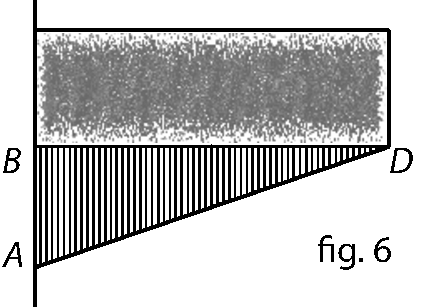
\includegraphics[width=0.52\textwidth]{gesamttex/edit_VIII,3/images/dnr-6a_LH_35_09_16_002-003_d6a.pdf}
\end{minipage}
\hspace{9mm}
\begin{minipage}[t]{0.5\textwidth}
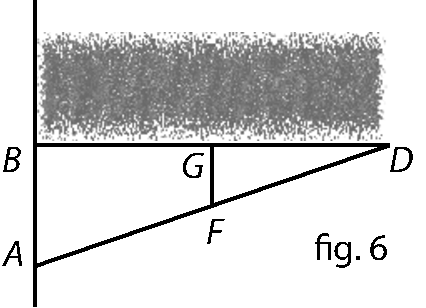
\includegraphics[width=0.51\textwidth]{gesamttex/edit_VIII,3/images/dnr-6b_LH_35_09_16_002-003_d6b.pdf}
\end{minipage}
\\
\\
\hspace*{9mm} [\textit{Fig.~6a, gestr.; L\textsuperscript{1}\,(Bl.~2~r\textsuperscript{o}\!)}]\hspace*{24mm} [\textit{Fig.~6b, gestr.; L\textsuperscript{1}\,(Bl.~2~r\textsuperscript{o}\!)}]
\pend
\vspace{1em}
\vspace{1.0em}%    % Diagramm Fig.~6c
  \centerline{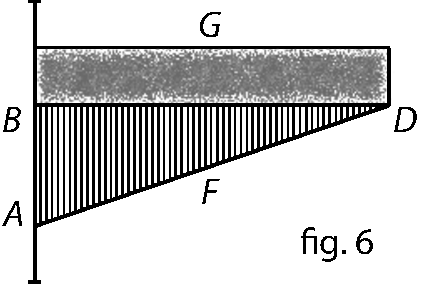
\includegraphics[width=0.32\textwidth]{gesamttex/edit_VIII,3/images/dnr-6c_AE_1684_319-325_d6c.pdf}}%\\
  \vspace*{0.05em}
  \centerline{\lbrack\textit{Fig.~6c; E\textsuperscript{1}}\rbrack}%
  \label{AE_1684_324_Fig.6} 
%%%%%%%%%%%%%%%%%%%%%%%%%%%%%%%%%%%%%%%%%%%%%%%%%%%%%%%%%%%%%%%%%%%%%%%%%%%%
\vspace{1.5em} 
\count\Bfootins=900
\count\Afootins=1000
\count\Cfootins=1000
\newpage%
%%%%%%%%%%%%%%%%%%%%%%%%%%%%%%%%ABBIldungen 6a 6b 6c%%%%%%%%%%%%%%%%%%%%%%%%%%%%%%%%%
%
%
%  \vspace*{2.0em}%    % Diagramm Fig.~6a
%  \centerline{\hspace*{-90mm}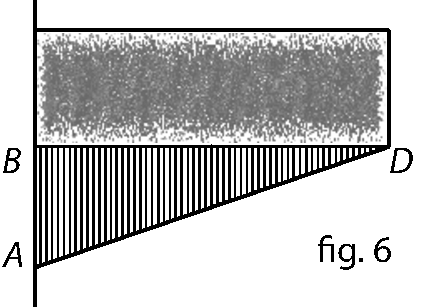
\includegraphics[width=0.24\textwidth]{gesamttex/edit_VIII,3/images/dnr-6a_LH_35_09_16_002-003_d6a.pdf}}%
%  \vspace*{0.5em}
%  \centerline{\hspace*{-90mm}\lbrack\textit{Fig.~6a, gestr.; L\textsuperscript{1}\,(Bl.~2~r\textsuperscript{o}\!)}\rbrack}%
%%  \label{}%
%%  \vspace{2em}%
%%  \newpage%
%%
%%
%%  \newpage% 
%  \vspace{-9.25em}%    % Diagramm Fig.~6b
%  \centerline{\hspace*{90mm}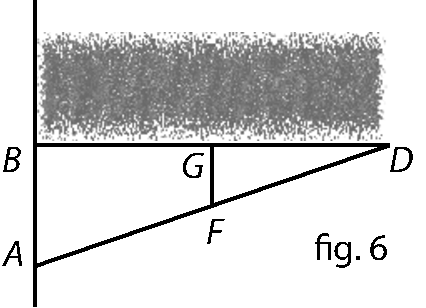
\includegraphics[width=0.24\textwidth]{gesamttex/edit_VIII,3/images/dnr-6b_LH_35_09_16_002-003_d6b.pdf}}%
%  \vspace*{0.5em}
%  \centerline{\hspace*{90mm}\lbrack\textit{Fig.~6b, gestr.; L\textsuperscript{1}\,(Bl.~2~r\textsuperscript{o}\!)}\rbrack}%
%%  \label{}%
%%  \vspace{2em}%
%%  \newpage%
%%
%%
%%  \newpage
%  \vspace{1.0em}%    % Diagramm Fig.~6c
%  \centerline{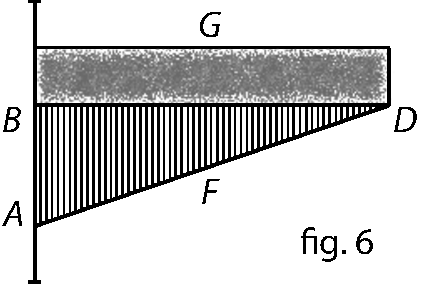
\includegraphics[width=0.32\textwidth]{gesamttex/edit_VIII,3/images/dnr-6c_AE_1684_319-325_d6c.pdf}}%\\
%  \vspace*{0.05em}
%  \centerline{\lbrack\textit{Fig.~6c; E\textsuperscript{1}}\rbrack}%
%  \label{AE_1684_324_Fig.6}
%%  \vspace*{0.0em}%
 %
% \pstart%
% % % % %    ACHTUNG GETRIXT: Diese Cfootnote bezieht sich eigentlich auf Fig.~6    ! ! ! ! 
% \edtext{}{%
% \lemma{\hspace{1,6mm}\lbrack\textit{Fig.~6a}\rbrack\ bis \lbrack\textit{Fig.~6c}\rbrack}\killnumber\Cfootnote{%
% Kein entsprechendes Diagramm ist in \textit{L\textsuperscript{2}} überliefert.}} %
% \pend%
%
%
  %\newpage%
  \centerline{%
  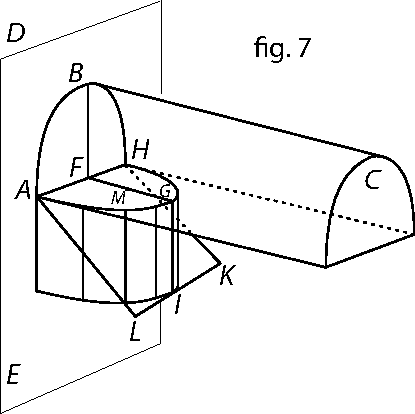
\includegraphics[width=0.42\textwidth]{gesamttex/edit_VIII,3/images/dnr-7a_LH_37_03_071-072+AE_1684_319-325_d7a.pdf}}%
  %\vspace{0.5em}
  \centerline{
  \lbrack\textit{Fig.~7a}\rbrack}%
  \label{AE_1684_324_Fig.7}%
 % \newpage
 \vspace{2.5em}
     \pstart% REIN VORLÄUFIG !!!
     \begin{minipage}[t]{0.5\textwidth}
  \hspace*{-6mm}
   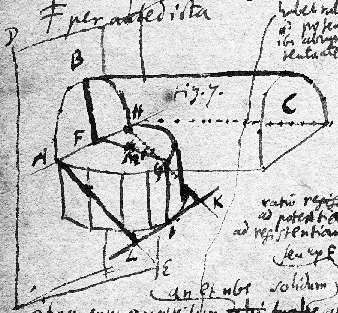
\includegraphics[width=0.82\textwidth]{gesamttex/edit_VIII,3/images/dnr-7b_LH_37_03_071-072_d7b.pdf}\\
  \newline
   \vspace*{1.0em}
   \hspace*{0mm}[\textit{Fig.~7b; nach L\textsuperscript{2}\,(Bl.~72~v\textsuperscript{o})}]
   \end{minipage}
   \begin{minipage}[t]{0.5\textwidth}
  \hspace*{0mm}
 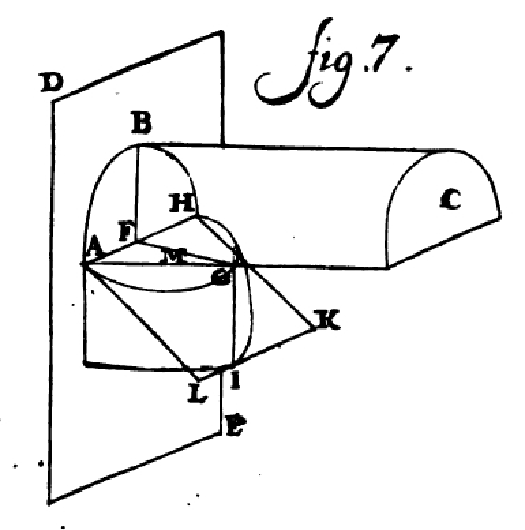
\includegraphics[width=0.83\textwidth]{gesamttex/edit_VIII,3/images/dnr-7c_AE_1684_319-325_d7c.pdf}\\
  \newline
   \vspace*{1.0em}
 \hspace*{15mm}[\textit{Fig.~7c; nach~E\textsuperscript{1}}]
  \end{minipage}
%
\edtext{}{\lemma{\hspace{1,6mm}\lbrack\textit{Fig.~7a}\rbrack}\killnumber\Cfootnote{%
Das Diagramm entspricht den Angaben auf S.~\refpassage{LH_37_03_072v+AE_1684_324-325_Fig.7-1}{LH_37_03_072v+AE_1684_324-325_Fig.7-2}.}}%
\edtext{}{\lemma{\hspace{1,6mm}\lbrack\textit{Fig.~7b}\rbrack\ und \lbrack\textit{Fig.~7c}\rbrack}\killnumber\Cfootnote{%
Beide Diagramme sind perspektivisch mangelhaft.
Die Zeichnung ist in \textit{L\textsuperscript{1}} nicht überliefert, wohl aber nahezu identisch im Brief an Mariotte vom März/April 1683 (\cite{01262}\textit{LSB} III,~3 N.~456, S.~797).}}%
 \pend%
% \vspace*{1.5em}%
\newpage
\pstart%
\edtext{}{%
{\xxref{LH_37_03_072v+AE_1684_324-325_ultimapars-1}{LH_37_03_072v+AE_1684_324-325_ultimapars-2}}%
\lemma{Hactenus}\Bfootnote{
\hspace{-0,5mm} autem
\lbrack...\rbrack\ unice desideratur.%
~\textit{fehlt~L\textsuperscript{1}}}}%
Hactenus\edlabel{LH_37_03_072v+AE_1684_324-325_ultimapars-1}
%%%%    GETRIXT MIT DER AUF FIG. 7 BEZOGENEN CFOOTNOTE
% \edtext{}{\lemma{\hspace{1,6mm}\lbrack\textit{Fig.~7b}\rbrack}\killnumber\Cfootnote{%
% Das Diagramm entspricht nicht der Beschreibung im Text (siehe unten, S.~\refpassage{LH_37_03_072v+AE_1684_324-325_Fig.7-1}{LH_37_03_072v+AE_1684_324-325_Fig.7-2}).}}
%%%%
% <<
\edtext{autem consideravimus tantum trabem,\protect\index{Sachverzeichnis}{trabs}
cujus superficies,\protect\index{Sachverzeichnis}{superficies trabis}
qua muro\protect\index{Sachverzeichnis}{murus}
vel sustentaculo\protect\index{Sachverzeichnis}{sustentaculum trabis} adhaeret,
ubique aeque alta est,
unde suffecit assumere rectam \textit{BA}, sed}{%
\lemma{autem}\Bfootnote{\hspace{-0,5mm}%
\textit{(1)}~solam lineam
\textit{(2)}~consideravimus tantum trabem cujus
\textit{(a)}~sectio communis cum muro est parallelogrammum
\textit{(b)}~superficies qua muro adhaeret
\textit{(c)}~alt
\textit{(d)}~superficies
\textit{(aa)}~qua muro adhaeret
\textit{(bb)}~qua muro vel sustentaculo adhaeret
\textit{(aaa)}~\textit{BA}
\textit{(bbb)}~, ubique aeque alta est, unde \textbar~hactenus \textit{gestr.}~\textbar\ suffecit assumere
\textit{(aaaa)}~lineam
\textit{(bbbb)}~rectam \textit{BA}. Sed%
~\textit{L\textsuperscript{2}}
\hspace{0,5mm}autem consideravimus \lbrack...\rbrack\ \textit{BA}, sed%
~\textit{E\textsuperscript{1}}}}
% >>
\makebox[1.0\textwidth][s]{quia superficies communis trabi\protect\index{Sachverzeichnis}{superficies trabis} et
% <
\edtext{parieti,\protect\index{Sachverzeichnis}{paries}}{%
\lemma{parieti~\textit{L\textsuperscript{2}}}\Bfootnote{%
\hspace{0,5mm}parieti~,~\textit{E\textsuperscript{1}}}}
% >
varia esse potest, demus regulam generalem\protect\index{Sachverzeichnis}{regula generalis geometrice determinanda}}
% >>>
\pend
 \pstart
\noindent
pro resistentia\protect\index{Sachverzeichnis}{resistentia trabis}
% <<
\edtext{ejus Geometrice determinanda,
cujus speciales casus\protect\index{Sachverzeichnis}{casus specialis} si cui pertractare vacabit,}{%
\lemma{ejus}\Bfootnote{\hspace{-0,5mm}%
\textit{(1)}~repraesent
\textit{(2)}~geometrice repraesentanda;
\textit{(a)}~qui si cujus vacabit speciales casus pertractare
\textit{(b)}~cujus speciales \lbrack...\rbrack\ pertractare vacabit% casus si cui
~\textit{L\textsuperscript{2}}
\hspace{0,5mm}ejus Geometrice \lbrack...\rbrack\ pertractare vacabit,%
~\textit{E\textsuperscript{1}}}}
% >>
is multa perelegantia theoremata\protect\index{Sachverzeichnis}{theorema perelegans} deprehendet.
In genere
% <
\edtext{autem,}{%
\lemma{autem~\textit{L\textsuperscript{2}}}\Bfootnote{%
\hspace{0,5mm}autem~,~\textit{E\textsuperscript{1}}}}
% >
sit \edlabel{LH_37_03_072v+AE_1684_324-325_Fig.7-1}trabs\protect\index{Sachverzeichnis}{trabs}
\textit{ABHC},\textso{ }%
\edtext{\textso{fig.}~\textso{7,}}{%
{\lemma{\textso{fig.}~\textso{7,}}\Bfootnote{%
\textit{erg.~L\textsuperscript{2}}}}%
{\lemma{\textso{fig.}~\textso{7}}\Cfootnote{%
Das Diagramm \lbrack\textit{Fig.~7a}\rbrack\ auf S.~\pageref{AE_1684_324_Fig.7}.}}}
% 
cujus sectio\protect\index{Sachverzeichnis}{sectio trabis}
\edtext{ad sustentaculum\protect\index{Sachverzeichnis}{sustentaculum trabis} \textit{DE}}{%
\lemma{ad}\Bfootnote{\hspace{-0,5mm}%
\textit{(1)}~murum\protect\index{Sachverzeichnis}{murus}
\textit{(2)}~sustentaculum \textit{DE}%
~\textit{L\textsuperscript{2}}}}
%
sit planum \textit{ABH} figurae cujuscunque.\protect\index{Sachverzeichnis}{figura}
Demittatur illud in horizontem,\protect\index{Sachverzeichnis}{horizon}
seu in plano horizontis\protect\index{Sachverzeichnis}{planum horizontis}
describatur aliud ei
% <
\edtext{aequale,}{%
\lemma{aequale~\textit{L\textsuperscript{2}}}\Bfootnote{%
\hspace{0,5mm}aequale~,~\textit{E\textsuperscript{1}}}}
% >
% <
\edtext{simile,}{%
\lemma{simile~\textit{L\textsuperscript{2}}}\Bfootnote{%
\hspace{0,5mm}simile~,~\textit{E\textsuperscript{1}}}}
% >
et similiter positum \textit{AGH}.
% <
\edtext{Ex puncto \textit{G}}{%
\lemma{Ex}\Bfootnote{% \hspace{-0,5mm}%
\textit{(1)}~\textit{A}
\textit{(2)}~puncto \textit{G}%
~\textit{L\textsuperscript{2}}}}
% >
ab \textit{AH}
% <
\edtext{horizontalium infima}{%
\lemma{horizontalium}\Bfootnote{%
\hspace{-0,5mm}infima
\textit{erg.~L\textsuperscript{2}}}}
% >
maxime remoto
(\protect\vphantom)%
quod respondet puncto \textit{B}%
\protect\vphantom()
ducatur ad \textit{AH} perpendicularis
% <<
\edtext{\textit{GF}
(\protect\vphantom)%
ipsi \textit{BF} aequalis%
\protect\vphantom()}{%
\lemma{\textit{GF}}\Bfootnote{\hspace{-0,5mm}%
\textit{(1)}~(\protect\vphantom)aequalis ipsi \textit{BF}\protect\vphantom()
\textit{(2)}~(\protect\vphantom)ipsi \textit{BF} aequalis\protect\vphantom()%
~\textit{L\textsuperscript{2}}}}
% >>
et fiat corpus cylindricum,
cujus basis aut sectio
%
\lbrack S.~325\rbrack\ % S.~325
%
quaecunque parallela horizonti sit similis et aequalis ipsi \textit{AGH},
altitudo autem perpendicularis sit \textit{GI}, aequalis
% <<
\edtext{\textit{FG} vel \textit{BF};
quod corpus liceat appellare cylindrum.\protect\index{Sachverzeichnis}{corpus cylindricum}}{%
\lemma{\textit{FG}}\Bfootnote{%
\hspace{-0,5mm}\textbar~vel \textit{BF} \textit{erg.}~%
% \textbar~; quod corpus liceat appellare cylindrum \textit{fehlt}~%
\textbar~.%
~\textit{L\textsuperscript{2}}
\hspace{0,5mm}\textit{FG} vel \lbrack...\rbrack\ appellare cylindrum.%
~\textit{E\textsuperscript{1}}}}
% >>
Per \textit{I} ducatur tangens indefinita \textit{KIL}\protect\index{Sachverzeichnis}{tangens indefinita}
parallela ipsi \textit{AH}.
Tandem
% <
\edtext{planum transeat}{%
\lemma{planum}\Bfootnote{% \hspace{-0,5mm}%
\textit{(1)}~quod transit
\textit{(2)}~transeat%
~\textit{L\textsuperscript{2}}}}
% >
per \textit{AH} et
% <
\edtext{\textit{KL},}{%
\lemma{\textit{KL}~\textit{L\textsuperscript{2}}}\Bfootnote{%
\hspace{0,5mm}\textit{KL}~,~\textit{E\textsuperscript{1}}}}
% >
quod ad horizontem\protect\index{Sachverzeichnis}{horizon}
faciet angulum
% <
\edtext{semirectum}{%
\lemma{semirectum~,~\textit{L\textsuperscript{2}}}\Bfootnote{%
\hspace{0,5mm}semirectum~\textit{E\textsuperscript{1}}}}
% >
et corpus cylindricum\protect\index{Sachverzeichnis}{corpus cylindricum} secabit in duas partes,
quarum illa in quam cadit
% <
\edtext{\textit{GI}, quae}{%
\lemma{\textit{GI}}\Bfootnote{% \hspace{-0,5mm}
seu quae%
~\textit{L\textsuperscript{2}}
\hspace{0,5mm}\textit{GI}~, quae%
~\textit{E\textsuperscript{1}}}}
% >
in figura est supra planum secans,\protect\index{Sachverzeichnis}{planum secans}
a Geometris\protect\index{Sachverzeichnis}{geometra} dicitur\textso{ }%
% <
\edtext{\textso{Ungula.}\protect\index{Sachverzeichnis}{ungula}}{%
\lemma{Ungula.~\textit{L\textsuperscript{2}}}\Bfootnote{%
\hspace{0,5mm}\textso{Ungula.}~\textit{E\textsuperscript{2}}}}%
\edlabel{LH_37_03_072v+AE_1684_324-325_Fig.7-2}
% >
Dico
% <<
\edtext{hanc Ungulam\protect\index{Sachverzeichnis}{ungula}
a cylindro\protect\index{Sachverzeichnis}{cylinder} resectam
facientem officium}{%
\lemma{hanc}\Bfootnote{%
\hspace{-0,5mm}$\langle$...$\rangle$ $\langle$facien$\rangle$tem $\langle$off$\rangle$icium%
~\textit{L\textsuperscript{2}}% \hspace{1,0mm}
% Ungulam a \lbrack...\rbrack\ facientem officium%
% ~\textit{E\textsuperscript{1}}
}}
% >>
vectis,\protect\index{Sachverzeichnis}{vectis}
cujus fulcrum\protect\index{Sachverzeichnis}{fulcrum vectis} sit in \textit{AH},
aequare vel repraesentare resistentiam trabis\protect\index{Sachverzeichnis}{resistentia trabis} \textit{ABHC}
% <<
\edtext{transversim in \textit{AHB} rumpendae,\protect\index{Sachverzeichnis}{trabs rumpenda}}{%
\lemma{transversim}\Bfootnote{%
\hspace{-0,5mm}\textbar~%
\textit{(1)}~ad murum
\textit{(2)}~in
\textit{(a)}~\textit{ABH}
\textit{(b)}~\textit{AHB} \textit{erg.}~%
\textbar\ rumpendae%
~\textit{L\textsuperscript{2}}
\hspace{0,5mm}transversim in \textit{AHB} rumpendae,%
~\textit{E\textsuperscript{1}}}}
% >>
si pondus\protect\index{Sachverzeichnis}{pondus evellens}
ipsius cylindri\protect\index{Sachverzeichnis}{cylinder} ad
% <
\edtext{eandem directe}{%
\lemma{eandem}\Bfootnote{%
\textit{(1)}~recta
\textit{(2)}~directe%
~\textit{L\textsuperscript{2}}}}
% >
ex muro\protect\index{Sachverzeichnis}{murus}
evellendam\protect\index{Sachverzeichnis}{trabs evellenda} sufficit.
Sed ne opus sit ungulam\protect\index{Sachverzeichnis}{ungula} considerari ad \makebox[1.0\textwidth][s]{modum vectis,\protect\index{Sachverzeichnis}{vectis}
et ut
% <
\edtext{pondus resistentiam\protect\index{Sachverzeichnis}{resistentia trabis}}{%
\lemma{pondus}\Bfootnote{%
\textit{(1)}~vim
\textit{(2)}~resistentiam%
~\textit{L\textsuperscript{2}}}}
% >
repraesentans absolute habeamus,
suspendatur}
\pend
\newpage
\pstart
\noindent  
ungula\protect\index{Sachverzeichnis}{ungula} ex
% <<
\edtext{}{{\xxref{KZeitz195}{KZeitz196}}%
{%
\lemma{puncto}\Bfootnote{%
\hspace{-0,5mm}\textit{M}
\textit{(1)}~respondente ejus centro gravitatis \textbar~et \textit{GH} \textit{erg.}~\textbar\
\textit{(2)}~seu ex \textit{FM}; distantia centri gravitatis ungulae a pariete%
~\textit{L\textsuperscript{2}}
\hspace{0,5mm}puncto \textit{M}, \lbrack...\rbrack\ a pariete;%
~\textit{E\textsuperscript{1}}}}}%
\edlabel{KZeitz195}puncto \textit{M},
seu ex \textit{FM} distantia centri gravitatis%
\protect\index{Sachverzeichnis}{centrum gravitatis ungulae}
ungulae\protect\index{Sachverzeichnis}{ungula}
a pariete;%
\protect\index{Sachverzeichnis}{paries}\edlabel{KZeitz196}
% >>
et ita
\edtext{exacte resistentiam transversalem\protect\index{Sachverzeichnis}{resistentia transversalis} aequabit,}{%
\lemma{exacte}\Bfootnote{%
\textit{(1)}~repraesentabit
\textit{(2)}~resistentiam transversalem aequabit,%
~\textit{L\textsuperscript{2}}}}
%
\edtext{si cylinder\protect\index{Sachverzeichnis}{cylinder}}{%
\lemma{si}\Bfootnote{%
\textlangle cylind\textrangle er%
~\textit{L\textsuperscript{2}}}}
%
totus
% <
\edtext{aequat direc\-tam.}{%
\lemma{aequat}\Bfootnote{\hspace{-0,5mm}%
\textit{(1)}~rectam
\textit{(2)}~\textlangle...\textrangle%
~\textit{L\textsuperscript{2}}
\hspace{0,5mm}aequat directam.%
~\textit{E\textsuperscript{1}}}}
% >
Itaque
% <
\edtext{cum quaeretur
an, et ubi solidum\protect\index{Sachverzeichnis}{solidum}}{%
\lemma{cum}\Bfootnote{\hspace{-0,5mm}%
\textit{(1)}~quaeritur
\textit{(2)}~quaeretur
\textit{(a)}~ubi trabs
\textit{(b)}~an et ubi solidum%
~\textit{L\textsuperscript{2}}
\hspace{0,5mm}cum quaeretur \lbrack...\rbrack\ ubi solidum%
~\textit{E\textsuperscript{1}}}}
% >
aliquod frangi debeat,
Geometrae\protect\index{Sachverzeichnis}{geometra} non
erit difficilis
% <
\edtext{aestimatio\protect\index{Sachverzeichnis}{aestimatio Geometrae};}{%
\lemma{aestimatio~,~\textit{L\textsuperscript{2}}}\Bfootnote{%
\hspace{0,5mm}aestimatio~;~\textit{E\textsuperscript{1}}}}
% >
id
% <<
\edtext{enim aut non aut ibi potissimum}{%
\lemma{enim}\Bfootnote{%
\hspace{-0,5mm}\textbar~aut non, aut potissimum \textit{erg.}~%
\textbar\ ibi%
~\textit{L\textsuperscript{2}}
\hspace{0,5mm}enim aut \lbrack...\rbrack\ ibi potissimum%
~\textit{E\textsuperscript{1}}}}
% >>
fiet,
% <<<
\edtext{ubi momentum ungulae,\protect\index{Sachverzeichnis}{momentum ungulae}
seu factum ex
\edtext{ungula\protect\index{Sachverzeichnis}{ungula}
ducta in distantiam sui centri \lbrack gravitatis\rbrack\protect\index{Sachverzeichnis}{centrum gravitatis ungulae}
a plano verticali
in quo est axis\protect\index{Sachverzeichnis}{axis librationis}
\edlabel{AE_1684_325,19_corrige-1}librationis\edlabel{AE_1684_325,19_corrige-2}\lbrack,\rbrack\
omnium minimam habebit rationem\protect\index{Sachverzeichnis}{ratio minima}}{%
\lemma{ungula \lbrack...\rbrack\ rationem}\Cfootnote{%
Laut \textit{LSB} III,~4 N.~72, S.~181.28\textendash32\cite{01257} soll der Satzteil folgendermaßen heißen:
\textit{ungula ducta in distantiam sui centri gravitatis a plano verticali
in quo est axis librationis, omnium minimum}\lbrack\textit{!}\rbrack\ \textit{habebit rationem}.
Nur teilweise ähnliche Verbesserungen sind in den 1693 veröffentlichten Korrigenda anzutreffen;
vgl. N.~14\textsubscript{10}, S.~\refpassage{AE_1684_325,19_corrige-3}{AE_1684_325,19_corrige-4}.}}
ad potentiam\protect\index{Sachverzeichnis}{potentia} ibi abrumpere tentantem:
ut}{%
\lemma{ubi}\Bfootnote{\hspace{-0,5mm}%
\textit{(1)}~factum ex ungula in
\textit{(2)}~momentum ungulae seu factum ex ungula
\textit{(a)}~in dista
\textit{(b)}~ducta in
\textit{(aa)}~\textit{FM}
\textit{(bb)}~distantiam sui centri gravitatis
\textit{(aaa)}~\textit{M}
\textit{(bbb)}~a recta 
\textit{(ccc)}~a plano \textit{AH}
\textit{(ddd)}~ab axe librationis
\textit{(eee)}~a plano in quo est axis librationis
\textit{(aaaa)}~\textit{AH}
\textit{(bbbb)}~erit omnium minimum.
\textit{(cccc)}~ratio
\textit{(aaaaa)}~resistentiae ad potentiam, seu
\textit{(bbbbb)}~potentiae ad resistentiam
\textit{(dddd)}~omnium minimam habet rationem ad \lbrack...\rbrack\ tentantem. Ut% potentiam ibi abrumpere
~\textit{L\textsuperscript{2}}
\hspace{0,5mm}ubi momentum \lbrack...\rbrack\ sui centri
\textbar~gravitatis, \textit{ändert Hrsg.}~%
\textbar\ a plano \lbrack...\rbrack\ tentantem: ut%
~\textit{E\textsuperscript{1}}}}
% >>>
proinde his paucis consideratis
tota haec materia\protect\index{Sachverzeichnis}{materia}
redacta sit ad puram Geometriam,\protect\index{Sachverzeichnis}{geometria pura}
quod in physicis\protect\index{Sachverzeichnis}{physica}
et mechanicis\protect\index{Sachverzeichnis}{mechanica} unice desideratur.%
\edlabel{LH_37_03_072v+AE_1684_324-325_ultimapars-2}%
\edlabel{DNDRS_L3fehlt_ukzck-2}
\pend%
\pstart%
\vspace{1.0em}
\noindent%
\lbrack\textit{Nachfolgender Textabschnitt ist lediglich in L\textsuperscript{3} und E\textsuperscript{1} überliefert:}\rbrack\
\pend%
\vspace{0.5em}%
%
\pstart%
\noindent%
\edtext{Additio:\protect\index{Sachverzeichnis}{additio}\edlabel{AE_1684_325_additio-1}
si quis
\edlabel{AE_1684_325,22_corrige-1}conoeides\protect\index{Sachverzeichnis}{conoeides}\edlabel{AE_1684_325,22_corrige-2}
%
\edtext{aliquod}{%
\lemma{aliquod}\Bfootnote{%
\textit{fehlt~L\textsuperscript{3}}}}
%
\edtext{quaerat,}{%
\lemma{quaerat~\textit{L\textsuperscript{3}}}\Bfootnote{%
\hspace{0,5mm}quaerat~,~\textit{E\textsuperscript{1}}}}
%
\edtext{aequalis resistentiae\protect\index{Sachverzeichnis}{resistentia trabis}}{%
\lemma{aequalis}\Bfootnote{%
\hspace{-0,5mm}ubique resistentiae;%
~\textit{L\textsuperscript{3}}
\hspace{0,5mm}
aequalis resistentiae%
~\textit{E\textsuperscript{1}}}}%
%
\lbrack,\rbrack\
huic satisfaciet Tuba parabolica.\protect\index{Sachverzeichnis}{tuba parabolica}
Sit in\textso{ }%
%
\edtext{\textso{fig.}~\textso{8,}}{%
{\lemma{\textso{fig.}~\textso{8,}}\Bfootnote{%
\textit{fehlt~L\textsuperscript{3}}}}%
{\lemma{\textso{fig.}~\textso{8}}\Cfootnote{%
Das Diagramm \lbrack\textit{Fig.~8b}\rbrack\ auf S.~\pageref{AE_1684_325_Fig.8b}.}}}
%
parabolica linea
%
\edtext{\textit{AEC}\protect\index{Sachverzeichnis}{linea parabolica}}{%
\lemma{\textit{AEC}~,~\textit{L\textsuperscript{3}}}\Bfootnote{%
\hspace{0,5mm}\textit{AEC}~\textit{E\textsuperscript{1}}}}
%
cujus vertex \textit{A},
tangens verticis \textit{AB},
circa quam tanquam
%
\edtext{axem,\protect\index{Sachverzeichnis}{axis}}{%
\lemma{axem~\textit{L\textsuperscript{3}}}\Bfootnote{%
\hspace{0,5mm}axem~,~\textit{E\textsuperscript{1}}}}
%
rotetur linea
%
\edtext{parabolica,\protect\index{Sachverzeichnis}{linea parabolica}}{%
\lemma{parabolica~;~\textit{L\textsuperscript{3}}}\Bfootnote{%
\hspace{0,5mm}parabolica~,~\textit{E\textsuperscript{1}}}}
%
et fiet
%
\edtext{Tuba \textit{AECGDFA}.\protect\index{Sachverzeichnis}{tuba parabolica}
Sumta}{%
\lemma{Tuba}\Bfootnote{\hspace{-0,5mm}%
\textbar~parabolica \textit{gestr.}~%
\textbar\ \textit{AECGDFA}.
\textit{(1)}~Sint
\textit{(2)}~Sumta%
~\textit{L\textsuperscript{3}}}}
%
jam adhuc
%
\edtext{alia Tubae portione}{%
\lemma{alia}\Bfootnote{%
\hspace{-0,5mm}portione Tubae%
~\textit{L\textsuperscript{3}}
\hspace{0,5mm}alia Tubae portione%
~\textit{E\textsuperscript{1}}}}
%
\textit{AEHFA},
cum resistentiae
%
\edtext{basium}{%
\lemma{basium~,~\textit{L\textsuperscript{3}}}\Bfootnote{%
\hspace{0,5mm}basium~\textit{E\textsuperscript{1}}}}
%
seu circulorum \textit{CGD},
%
\edtext{\textit{EHF}}{%
\lemma{\textit{EHF}~,~\textit{L\textsuperscript{3}}}\Bfootnote{%
\hspace{0,5mm}\textit{EHF}~\textit{E\textsuperscript{1}}}}
%
sint ut\protect\index{Sachverzeichnis}{cubus}
%
\edtext{Cubi}{%
\lemma{cubi~\textit{L\textsuperscript{3}}}\Bfootnote{%
\hspace{0,5mm}Cubi~\textit{E\textsuperscript{1}}}}
%
diametrorum \textit{CD},
%
\edtext{\textit{EF};}{%
\lemma{\textit{EF}~,~\textit{L\textsuperscript{3}}}\Bfootnote{%
\hspace{0,5mm}\textit{EF}~;~\textit{E\textsuperscript{1}}}}
%
\edtext{reperietur,}{%
\lemma{reperietur~\textit{L\textsuperscript{3}}}\Bfootnote{%
\hspace{0,5mm}reperietur~; \textit{E\textsuperscript{1}}}}
%
momenta ipsarum portionum \textit{AECGDFA} et \textit{AEHFA}\protect\index{Sachverzeichnis}{momentum tubae parabolicae}
ex natura parabolae\protect\index{Sachverzeichnis}{natura parabolae}\protect\index{Sachverzeichnis}{parabola}
esse etiam ut cubos \textit{CD}, \textit{EF}.\protect\index{Sachverzeichnis}{cubus}%
\edlabel{AE_1684_325_additio-2}}{%
\lemma{Additio:}\Bfootnote{%
\hspace{-0,5mm}si quis \lbrack...\rbrack\ cubos \textit{CD}, \textit{EF}.
\textit{fehlt~L\textsuperscript{1}\!\! u.\! L\textsuperscript{2}}}}
\pend%
\newpage
\pstart 
\begin{minipage}[t]{0.5\textwidth}
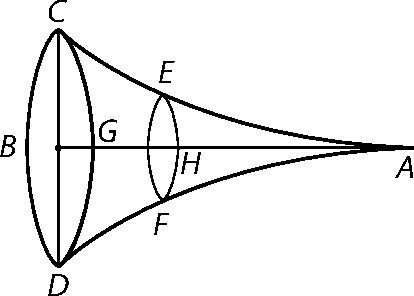
\includegraphics[width=0.74\textwidth]{gesamttex/edit_VIII,3/images/dnr-8a_LH_35_09_14_003r_d8a.pdf}
\end{minipage}
\hspace{1mm}
\begin{minipage}[t]{0.5\textwidth}
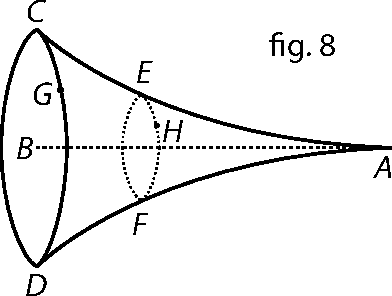
\includegraphics[width=0.7\textwidth]{gesamttex/edit_VIII,3/images/dnr-8b_AE_1684_319-325_d8b.pdf}
\end{minipage}
\\
\\
\hspace*{18mm} [\textit{Fig.~8a; L\textsuperscript{3}\,(Bl.~3~r\textsuperscript{o}\!)}] \label{LH_35_09_14_003r_bis_Fig.8a}\hspace*{42mm} [\textit{Fig.~8b; E\textsuperscript{1}}] \label{AE_1684_325_Fig.8b}
\pend
%\vspace{1em}
%
%
%%  \newpage
%  \vspace*{2.0em}%  REIN VORLÄUFIG
%%
%  \centerline{\hspace*{-70mm}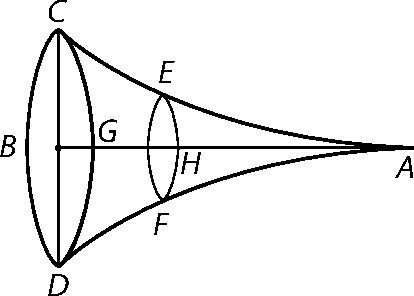
\includegraphics[width=0.34\textwidth]{gesamttex/edit_VIII,3/images/dnr-8a_LH_35_09_14_003r_d8a.pdf}}%\\
%  \vspace*{0.0em}
%  \centerline{\hspace*{-65mm}\lbrack\textit{Fig.~8a; L\textsuperscript{3}\,(Bl.~3~r\textsuperscript{o}\!)}\rbrack}%
%  \label{LH_35_09_14_003r_bis_Fig.8a}
%%
%  \vspace*{-11.0em}%  REIN VORLÄUFIG
%%
%  \centerline{\hspace*{75mm}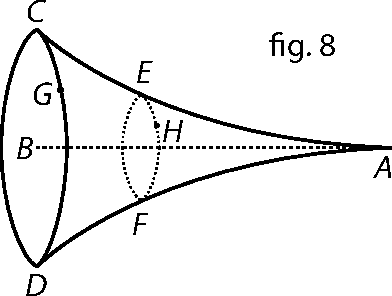
\includegraphics[width=0.32\textwidth]{gesamttex/edit_VIII,3/images/dnr-8b_AE_1684_319-325_d8b.pdf}}%\\
%  \vspace*{0.0em}
%  \centerline{\hspace*{75mm}\lbrack\textit{Fig.~8b; E\textsuperscript{1}}\rbrack}%
%  \label{AE_1684_325_Fig.8b}
%%
%
  %  %  %     ACHTUNG GETRIXT: Folgende Cfootnote bezieht sich auf Fig. 8
\pstart%
\phantom{Cfootnote zu Fig. 8}%
\edtext{}{%
\lemma{\hspace{1,6mm}\lbrack\textit{Fig.~8a}\rbrack\ und \lbrack\textit{Fig.~8b}\rbrack}%
\killnumber\Cfootnote{%
Kein entsprechendes Diagramm ist in \textit{L\textsuperscript{1}} oder \textit{L\textsuperscript{2}} überliefert.%
% \textit{Additio} (S.~\refpassage{AE_1684_325_additio-1}{AE_1684_325_additio-2})
}}
\pend
\count\Bfootins=1200
\count\Afootins=1200
\count\Cfootins=1200%
%  %  %  %
%
%
%
% ENDE DES STÜCKES auf Blatt 72v und S. 325
%
%
% \newpage%  Rein vorläufig !!!!
%